%@HEADER
% ************************************************************************
% 
%          Trilinos: An Object-Oriented Solver Framework
%              Copyright (2001) Sandia Corporation
% 
% Under terms of Contract DE-AC04-94AL85000, there is a non-exclusive
% license for use of this work by or on behalf of the U.S. Government.
% 
% This program is free software; you can redistribute it and/or modify
% it under the terms of the GNU General Public License as published by
% the Free Software Foundation; either version 2, or (at your option)
% any later version.
%   
% This program is distributed in the hope that it will be useful, but
% WITHOUT ANY WARRANTY; without even the implied warranty of
% MERCHANTABILITY or FITNESS FOR A PARTICULAR PURPOSE.  See the GNU
% General Public License for more details.
%   
% You should have received a copy of the GNU General Public License
% along with this program; if not, write to the Free Software
% Foundation, Inc., 675 Mass Ave, Cambridge, MA 02139, USA.
% 
% Questions? Contact Michael A. Heroux (maherou@sandia.gov)
% 
% ************************************************************************
%@HEADER

\documentclass[10pt]{report}
\usepackage{graphicx}
\usepackage{amsmath,amsfonts,amsthm}
\usepackage{amssymb}

\usepackage{times}

\setlength\oddsidemargin {-0pt}\setlength\evensidemargin{-0pt}
\setlength{\textwidth}{150mm}\setlength{\textheight}{210mm}
\headheight=12.45pt

\newcommand{\TriExe}[1]{{\tt\$\{TRILINOS\_HOME\}/doc/tutorial/ #1}}
\author{MS, ...}

%%%
%%% this is me
%%%


\newcommand{\Trilinos}{Trilinos}
\newcommand{\TrilinosTM}{Trilinos \copyright}

\newtheorem{remark}{Remark}

\begin{document}

\title{Trilinos 3.1 Tutorial, \\ version 0.9}
\maketitle

% Set to roman page numbers for front matter
%\pagenumbering{roman}

% Reset the margins for the remainder of the document
%\setlength{\oddsidemargin}{0.25in}
%\setlength{\evensidemargin}{0.25in}

\begin{abstract}
%\abstract*{Abstract}
%\section{Abstract}
  
  This document introduces the use of \Trilinos{}, version 3.1.
  \Trilinos{} has been written to support, in a rigorous manner, the
  solver needs of the engineering and scientific applications at Sandia
  National Laboratories.

  \medskip
  
  Aim of this manuscript is to present the basic features of some of the
  Trilinos packages. The presented material includes the definition of
  distributed matrices and vectors with Epetra, the iterative solution
  of linear system with AztecOO, incomplete factorizations with IFPACK,
  multilevel methods with ML, direct solution of linear system with
  Amesos, and iterative solution of nonlinear systems with NOX. With the
  help of several examples, some of the most important classes and
  methods are detailed to the unexperienced user.  For the most
  majority, each example is largely commented throughout the text. Other
  comments can be found in the source of each example.

  \medskip
  
  This document is a companion to the Trilinos User's
  Guide~\cite{Trilinos-Users-Guide} and Trilinos Development
  Guides~\cite{Trilinos-Dev-Guide,Trilinos-Dev-Guide-II}. Also, the
  documentation included in each of the Trilinos' packages is of
  fundamental importance.
 
\end{abstract}

\newpage
\clearpage

\tableofcontents

\clearpage

%@HEADER
% ************************************************************************
% 
%          Trilinos: An Object-Oriented Solver Framework
%              Copyright (2001) Sandia Corporation
% 
% Under terms of Contract DE-AC04-94AL85000, there is a non-exclusive
% license for use of this work by or on behalf of the U.S. Government.
% 
% This program is free software; you can redistribute it and/or modify
% it under the terms of the GNU General Public License as published by
% the Free Software Foundation; either version 2, or (at your option)
% any later version.
%   
% This program is distributed in the hope that it will be useful, but
% WITHOUT ANY WARRANTY; without even the implied warranty of
% MERCHANTABILITY or FITNESS FOR A PARTICULAR PURPOSE.  See the GNU
% General Public License for more details.
%   
% You should have received a copy of the GNU General Public License
% along with this program; if not, write to the Free Software
% Foundation, Inc., 675 Mass Ave, Cambridge, MA 02139, USA.
% 
% Questions? Contact Michael A. Heroux (maherou@sandia.gov)
% 
% ************************************************************************
%@HEADER

\section{Introduction}

The Trilinos Project is an effort to facilitate the design, development,
integration and ongoing support of mathematical software libraries.
Goal of the Trilinos Project is develop parallel solver algorithms and
libraries within an object-oriented software framework for the solution
of large-scale, complex multiphysics engineering and scientific
applications. The emphasis is on developing robust, scalable algorithm
in a software framework, using abstract interfaces for flexible
interoperability of components while providing a full-featured set of
concrete classes that implement all abstract interfaces.

%%%
%%%
%%%

\subsection{Getting Started with Trilinos}
\label{sec:getting}

The Trilinos Project uses a two-level software structure designed around
collections of packages. A Trilinos package is an integral unit, usually
developed to solve a specific task, by a (relatively) small group of
expert of the field.  Packages exist underneath the Trilinos top level,
which provides a common look-and-feel. Each package has its own
structure, documentation and set of examples. In principle, Trilinos
packages can live independently. However, each package is even more
valuable when combined with other Trilinos packages.

\smallskip

Trilinos is a large software project, and currently about twenty
packages are included. Fully understanding all the functionalities of
the Trilinos packages requires time. The entire set of packages covers a
wide range of numerical methods for large scale computing. Some packages
are focused on the development of computational schemes, like for
instance the solution of linear and nonlinear systems, to the definition
of parallel preconditioners for Krylov methods, eigenvalue computation.
Other packages are more focused on implementation issues (like
definition of matrices and vectors, abstract classes for linear
operators). The first Chapters of this tutorial will be focused on
implementation issues, while the last Chapters will have a more
``mathematical'' taste.

Each package offers sophisticated features, that cannot be ``unleashed''
at a very first usage. For each package, we will outline only the basic
features, and we refer to the documentation of each package for a more
involved usage. Our goal is to present enough material so that the
reader can successfully use the described packages.  In fact, for new
users, it is neither easy, nor necessary, to manage all the Trilinos
functionalities. At the beginning, it is more important for them to
understand how to manage the basic classes, such as vector, matrix and
linear system classes. However, it is clear that for a fine-tuning, the
reader will have to look through each package's documentation and
examples.

\medskip

Although all packages have the same importance in the Trilinos
structure, a typical user will probably --- at least at the beginning
--- make use of the following packages:
\begin{itemize} 
\item {\bf Epetra}. This package defines the basic classes for
  distributed matrices and vectors, linear operators and linear
  problems. Epetra classes are the common language spoken by all the
  Trilinos packages (even if some of them can ``speak'' other
  languages). Each Trilinos package is able to accept in input Epetra
  objects. This allows powerful combinations among the various Trilinos
  functionalities.
\item {\bf AztecOO}. This is a linear solve package based on
  preconditioned Krylov methods. It supports all the Aztec interfaces
  and functionality, but also provides significant new functionality.
\item {\bf IFPACK}. This is a package to perform various incomplete
  factorizations, and it is here used in conjunction with AztecOO.
\item {\bf ML}. This is an algebraic multilevel preconditioner package, which
  provided scalable preconditioning capabilities for a variety of
  problem classes. It is here used in conjunction with AztecOO.
\item {\bf Amesos}. This package provides a common interface to various
  direct solvers (generally available outside the Trilinos framework),
  both sequential and parallel.
\item {\bf NOX}. This is a collection of nonlinear solvers, designed to
  be easily integrated into an application and used with many different
  linear solvers.
\item {\bf Triutils}. This is a collection of various utilities, that
  can be extremely useful in some phases of software development.
\end{itemize}

Table~\ref{tab:tripackages} gives a partial overview of what can be
accomplished using Trilinos.
\begin{table}[htbp]
  \centering
  \begin{tabular}{| p{10cm} | p{3cm} |}
    \hline
    {\bf Task} & {\bf Package} \\
    \hline
    Light-weight interface to BLAS and LAPACK: & Epetra, Teuchos$^\star$ \\\hline
    Definition of serial dense or sparse matrices: & Epetra \\\hline
    Definition of distributed sparse matrices:& Epetra \\\hline
    solve a linear system with preconditioned Krylov accelerators, like
    CG, GMRES, Bi-CGSTAB, TFQMR:& AztecOO, Belos$^\star$ \\\hline
    Definition of incomplete factorizations:& AztecOO, \newline IFPACK \\\hline
    Definition of a multilevel preconditioner:& ML \\\hline
    Definition of a one-level Schwarz preconditioner (overlapping domain
    decomposition):& AztecOO, \newline IFPACK \\\hline
    Definition a two-level Schwarz preconditioner, with coarse grid based on
    aggregation:& AztecOO+ML \\\hline
    Solution of  systems of nonlinear equations:& NOX \\\hline
    interface with various direct solvers, as UMFPACK, MUMPS, SuperLU
    and others :& Amesos \\\hline
    Computation of eigenvalue of large, sparse matrices:& Anasazi$^\star$
    \\\hline
    Solution of complex linear equations (using equivalent real formulation):&
    Komplex$^\star$ \\\hline
    Definition of segregated preconditioners and block preconditioners (for
    instance, for the incompressible Navier-Stokes equations):&
    Meros$^\star$ \\\hline
    Templated interface to BLAS and LAPACK, arbitrary-precision
    arithmetic, parameter lists:& Teuchos$^\star$ \\\hline
    Definition of abstract interfaces to vectors, linear operators, and solvers:& TSF$^\star$, TSFCore$^\star$, TSFExtended$^\star$    \\
    \hline
  \end{tabular}
  \caption{Partial overview of what can be done with Trilinos. $\star$:
    not covered in this tutorial.}
  \label{tab:tripackages}
\end{table}

This tutorial is divided into 10 chapters:
\begin{itemize}
\item Chapter \ref{chap:epetra_vec} describes the Epetra\_Vector class;
\item Chapter \ref{chap:epetra_mat} introduces the Epetra\_Matrix
  class; 
\item Chapter \ref{chap:epetra_others} briefly describes some other
  Epetra classes;
\item Chapter \ref{chap:aztecoo} shows how to solve linear systems with
  AztecOO;
\item Chapter \ref{chap:ifpack} presents the basic usage of IFPACK;
\item Chapter \ref{chap:ml} introduces multilevel preconditioners based
  on ML;
\item Chapter \ref{chap:amesos} introduces the Amesos package;
\item Chapter \ref{chap:nox} outlines the main features of the Trilinos
  nonlinear solver package, NOX.
\item Chapter \ref{chap:triutils} presents some tools provided with the
  Triutils package. 
\end{itemize}

\begin{remark}
  As already pointed out, Epetra objects are meant to be the ``common
  language'' spoken by all the Trilinos packages, and therefore the new
  user must become familiar with those objects. Therefore we suggest to
  read Chapters \ref{chap:epetra_vec}-\ref{chap:epetra_others} before
  considering other Trilinos packages. Also, Chapter~\ref{chap:aztecoo}
  should be read before Chapters~\ref{chap:ifpack} and~\ref{chap:ml}
  (even if both IFPACK and ML can be compiled and run without AztecOO).
\end{remark}

This tutorial assume a basic background in numerical methods for PDEs,
and in iterative linear and nonlinear solvers. Although not strictly
necessary, the reader is suppose to have a certain familiarity with
distributed memory computing and, to a minor extent, with MPI.

\smallskip

Note that this tutorial is not a substitute ofr individual packages
documentation. Also, for an overview of all the Trilinos packages, the
Trilinos philosophy, and a description of the packages provided by
Trilinos, the reader is referred to \cite{Trilinos-Overview}.
Developers should also consider the Trilinos Developers' Guide, which
addresses many topics, including the development tools used by Trilinos'
developers, and how to include a new package\footnote{ Trilinos provides
  a variety of services to a developer wanting to integrate a package
  into Trilinos.  They include Autoconf~\cite{Autoconf},
  Automake~\cite{Automake} and Libtool~\cite{Libtool}. Those tools
  provide a robust, full-featured set of tools for building software
  across a broad set of platforms.  Although these tools are not
  official standards, they are widely used.  All existing Trilinos
  packages use Autoconf and Automake.  Libtool support will be added in
  future releases.}.

%%%
%%%
%%%

\subsection{Installing Trilinos}
\label{sec:installing}

To obtain Trilinos, please refers to the instructions reported at the
following web site:
\begin{verbatim}
http://software.sandia.gov/Trilinos
\end{verbatim}

Trilinos has been compiled on a variety of architectures, including
Linux, Sun Solaris, SGI Irix, DEC, and many others. Trilinos has been
designed to support parallel applications. However, it can be compiled
and run on serial computer.  Detailed comments on the installation, and
an exhaustive list of FAQs, can be found at the web pages:
\begin{verbatim}
http://software.sandia.gov/Trilinos/installing_manual.html
http://software.sandia.gov/Trilinos/faq.html
\end{verbatim}


Before using Trilinos, users might decide to set the environmental
variables \verb!TRILINOS_HOME!, indicating the full path of the Trilinos
directory, \verb!TRILINOS_LIB!, indicating the location of the compiled
Trilinos library, and \verb!TRILINOS_ARCH!, containing the architecture
and the communicator currently used.  For example, using the BASH shell,
command lines of the form
\begin{verbatim}
export TRILINOS_HOME=/home/msala/Trilinos
export TRILINOS_ARCH=LINUX.MPI
export TRILINOS_LIB=${TRILINOS_HOME}/${TRILINOS_ARCH}
\end{verbatim}
can be places in the users' \verb!.bashrc! file.

\smallskip

Here, we briefly report the procedure one should follow in order to
compile Trilinos as required by the examples reported in the following
chapters \ref{chap:epetra_vec}-\ref{chap:triutils}\footnote{Amesos can
  be more difficult to compile for the unexperienced user, as it
  required some information about the packages to interface. Suggestions
  about the configuration of Amesos are reported in
  Chapter~\ref{chap:amesos}. More details about the installation of
  Trilinos can be found in \cite{Trilinos-Users-Guide}.}.  Suppose we
want to compile under LINUX with MPI. The installation procedure can be
are reported below. (\verb!$! indicates the shell prompt.)
\begin{verbatim}
$ cd ${TRILINOS_HOME}
$ mkdir ${TRILINOS_ARCH}
$ cd ${TRILINOS_ARCH}
$ ../configure --prefix="${TRILINOS_HOME}/${TRILINOS_ARCH}" \
  --enable-mpi --with-mpi-compilers \
  --enable-triutils --enable-aztecoo \
  --enable-ifpack \
  --enable-ml --enable-nox | tee configure_${TRILINOS_ARCH}.log
$ make | tee make_${TRILINOS_ARCH}.log
$ make install | tee make_install_${TRILINOS_ARCH}.log
\end{verbatim}

\begin{remark}
  All Trilinos packages can be build to run with or without MPI. If MPI
  is enabled (using \verb!--enable-mpi!), the users must know the
  procedure for beginning MPI jobs on their computer system(s). In some
  cases, options must be set on the configure line to specify the
  location of MPI include files and libraries.
\end{remark}

%%%
%%%
%%%

\subsection{Compiling and Linking a program using Trilinos}
\label{sec:intro_compiling}

In order to compile and link (part of) the Trilinos library, the use can
decide to use a Makefile as reported below. This Makefile refers to one
of the examples, reported in the NOX subdirectory of this tutorial.
\begin{verbatim}
 1: TRILINOS_HOME = /home/msala/Trilinos/
 2: TRILINOS_ARCH - LINUX_MPI
 3: TRILINOS_LIB = $(TRILINOS_HOME)$(TRILINOS_ARCH)
 4: 
 5: include $(TRILINOS_HOME)/build/makefile.$(TRILINOS_ARCH)
 6: 
 7: MY_COMPILER_FLAGS = -DHAVE_CONFIG_H $(CXXFLAGS) -c -g\
 8:                    -I$(TRILINOS_LIB)/include/
 9:
10: MY_LINKER_FLAGS = $(LDFLAGS) $(TEST_C_OBJ) \
11:         -L$(TRILINOS_LIB)/lib/ \
12:         -lnoxepetra -lnox -lifpack \
13:         -laztecoo -lepetra -llapack -lblas $(ARCH_LIBS)
14:
15: ex1: ex1.cpp
16:         $(CXX)     ex1.cpp $(MY_COMPILER_FLAGS)
17:         $(LINKER)  ex1.o   $(MY_LINKER_FLAGS)    -o ex1.exe
\end{verbatim}

Line number have been reported for  reader's convenience. 

The lines 1-3 can be omitted, see Section \ref{sec:installing}.  Line 5
includes basic definitions of Trilinos. (Note that, on some
architectures, one may need to use \verb!gmake! instead of \verb!make!.)
In line 7, the variable \verb!HAVE_CONFIG_H! is defined. Linker flags of
lines 10-13 defines the library to link (location of BLAS and LAPACK can
change on different platforms). The variable \verb!ARCH_LIBS! is defined
in line 5.

To run the compiled example in a sequential environment, simply type
\begin{verbatim}
$ ./ex1.exe
\end{verbatim}
In a MPI environment, the user might have to
use an instruction of type
\begin{verbatim}
$ mpirun -np 2 ./ex1.exe
\end{verbatim}
Please check the local MPI documentation for more details. 

%%%
%%%
%%%

\subsection{Copyright and Licensing of Trilinos}
\label{sec:copyright}

Trilinos is released under the Lesser GPL GNU Licence.

Trilinos is copyrighted by Sandia Corporation. Under the terms of
Contract DE-AC04-94AL85000, there is a non-exclusive license for use of
this work by or on behalf of the U.S. Government.  Export of this
program may require a license from the United States Government.

NOTICE: The United States Government is granted for itself and others
acting on its behalf a paid-up, nonexclusive, irrevocable worldwide
license in ths data to reproduce, prepare derivative works, and perform
publicly and display publicly.  Beginning five (5) years from July 25,
2001, the United States Government is granted for itself and others
acting on its behalf a paid-up, nonexclusive, irrevocable worldwide
license in this data to reproduce, prepare derivative works, distribute
copies to the public, perform publicly and display publicly, and to
permit others to do so.

NEITHER THE UNITED STATES GOVERNMENT, NOR THE UNITED STATES DEPARTMENT
OF ENERGY, NOR SANDIA CORPORATION, NOR ANY OF THEIR EMPLOYEES, MAKES ANY
WARRANTY, EXPRESS OR IMPLIED, OR ASSUMES ANY LEGAL LIABILITY OR
RESPONSIBILITY FOR THE ACCURACY, COMPLETENESS, OR USEFULNESS OF ANY
INFORMATION, APPARATUS, PRODUCT, OR PROCESS DISCLOSED, OR REPRESENTS
THAT ITS USE WOULD NOT INFRINGE PRIVATELY OWNED RIGHTS.

\medskip

Some parts of Trilinos are dependent on a third party code. Each third
party code comes with its own copyright and/or licensing requirements.
It is responsibility of the user to understand these requirements.

%%%
%%%
%%%

\subsection{Programming Language Used in this Tutorial}
\label{sec:language}

Trilinos is written in C++ (for most packages), and in C. Some
interfaces are provided to FORTRAN code (mainly BLAS and LAPACK
routines). Even if a limited support is included for C programs (and a
more limited for FORTRAN code), to unleashed the full power of Trilinos
we suggest to use C++. All the example programs contained in this
tutorial will be in C++; some packages contains examples in C.

%%%
%%%
%%%

\subsection{Referencing Trilinos}
\label{sec:referencing}

The Trilinos project can be referenced by using the following BiBTeX
citation information:
\begin{verbatim}
@techreport{Trilinos-Overview,
title = "{An Overview of Trilinos}",
author = "Michael Heroux and Roscoe Bartlett and Vicki Howle
Robert Hoekstra and Jonathan Hu and Tamara Kolda and
Richard Lehoucq and Kevin Long and Roger Pawlowski and
Eric Phipps and Andrew Salinger and Heidi Thornquist and
Ray Tuminaro and James Willenbring and Alan Williams ",
institution = "Sandia National Laboratories",
number = "SAND2003-2927",
year = 2003}

@techreport{Trilinos-Dev-Guide,
title = "{Trilinos Developers Guide}",
author = "Michael A. Heroux and James M. Willenbring and Robert Heaphy",
institution = "Sandia National Laboratories",
number = "SAND2003-1898",
year = 2003}

@techreport{Trilinos-Dev-Guide-II,
title = "{Trilinos Developers Guide Part II: ASCI Software Quality
Engineering Practices Version 1.0}",
author = "Michael A. Heroux and James M. Willenbring and Robert Heaphy",
institution = "Sandia National Laboratories",
number = "SAND2003-1899",
year = 2003}

@techreport{Trilinos-Users-Guide,
title = "{Trilinos Users Guide}",
author = "Michael A. Heroux and James M. Willenbring",
institution = "Sandia National Laboratories",
number = "SAND2003-2952",
year = 2003}
\end{verbatim}
These BiBTeX information can be downloaded from the web page

\begin{verb}
http://software.sandia.gov/Trilinos/citing.html
\end{verb}

%%%
%%%
%%%

\subsection{A Note on Directory Structure}
\label{sec:into_note}

Each Trilinos package in contained in the subdirectory
\begin{verbatim}
${TRILINOS_HOME}/packages
\end{verbatim}
The structure of all packages is quite similar (although not exactly
equal). As a general line, source files are in
\begin{verbatim}
${TRILINOS_HOME}/packages/<package-name>/src
\end{verbatim}
Example files are reported in \begin{verbatim}
${TRILINOS_HOME}/packages/<package-name>/examples
\end{verbatim}
and test files in
\begin{verbatim}
${TRILINOS_HOME}/packages/<package-name>/test
\end{verbatim}
The documentation is reported
\begin{verbatim}
${TRILINOS_HOME}/packages/<package-name>/doc
\end{verbatim}
Often, Trilinos developers use Doxygen\footnote{Copyright \copyright
  1997-2003 by Dimitri van Heesch. More information can by found at the
  web address {\tt http://www.stack.nl/~dimitri/doxygen/}.}. For
instance, to create the documentation for Epetra, we use can type
\begin{verbatim}
$ cd ${TRILINOS_HOME}/packages/epetra/doc
$ doxygen Doxyfile
\end{verbatim}
and then browse it using an HTML reader, or compiling the \LaTeX file
using
\begin{verbatim}
$ cd ${TRILINOS_HOME}/packages/epetra/doc/latex
$ make
\end{verbatim}

%%%
%%%
%%%

\subsection{List of Trilinos Developers}
\label{sec:intro_incomplete}

A list of the Trilinos' developers, updated to December 2003, would
include the following names (in alphabetical order):

Roscoe A. Bartlett,
Jason A. Cross,
David M. Day,
Robert Heaphy,
Michael A. Heroux (project leader),
Russell Hooper,
Vicki E. Howle,
Robert J. Hoekstra,
Jonathan J. Hu,
Tamara G. Kolda,
Richard B. Lehoucq,
Paul Lin,
Kevin R. Long,
Roger P. Pawlowski,
Michael N. Phenow,
Eric T. Phipps,
Andrew J. Rothfuss,
Marzio Sala,
Andrew G. Salinger,
Paul M. Sexton,
Kendall S. Stanley,
Heidi K. Thornquist,
Ray S. Tuminaro,
James M. Willenbring,
Alan Williams.



\include{getting_started}

%@HEADER
% ************************************************************************
% 
%          Trilinos: An Object-Oriented Solver Framework
%              Copyright (2001) Sandia Corporation
% 
% Under terms of Contract DE-AC04-94AL85000, there is a non-exclusive
% license for use of this work by or on behalf of the U.S. Government.
% 
% This program is free software; you can redistribute it and/or modify
% it under the terms of the GNU General Public License as published by
% the Free Software Foundation; either version 2, or (at your option)
% any later version.
%   
% This program is distributed in the hope that it will be useful, but
% WITHOUT ANY WARRANTY; without even the implied warranty of
% MERCHANTABILITY or FITNESS FOR A PARTICULAR PURPOSE.  See the GNU
% General Public License for more details.
%   
% You should have received a copy of the GNU General Public License
% along with this program; if not, write to the Free Software
% Foundation, Inc., 675 Mass Ave, Cambridge, MA 02139, USA.
% 
% Questions? Contact Michael A. Heroux (maherou@sandia.gov)
% 
% ************************************************************************
%@HEADER

\section{Working with Epetra Vectors}
\label{chap:epetra_vec}

Probably, the first mathematical entities defined by a numerical method
is a vector. Within the Trilinos framework, vectors are usually
constructed starting from Epetra Classes.

Epetra vectors can be used to store double values (like the solution of
a PDE problem, the right-hand side of a linear system, or the nodal
coordinates), as well as integer data values (such as a set of indexes).

Epetra vectors can be {\em serial} or {\em distributed}. Serial vectors
are usually small, so that it is not convenient to distribute them
across the processes. Possibly, serial vectors are replicated across the
processes. On the other hand, distributed vectors tend to be
significantly larger, and therefore their elements are distributed
across the processors. In this latter case, users must specify the
partition they intend to use.  In Epetra, this is done by specifying a
communicator (introduced in Section~\ref{sec:comm}) and an Epetra object
called map (introduced in Section~\ref{sec:map}). A map is basically a
partitioning of a list of global IDs.

\medskip

This Chapter will show some of the Trilinos capabilities to work with
vectors. Vector classed can be used to perform common vector operations,
as dot products, vector scalings and norms, or fill with constant or
random values. 

\medskip

During the Chapter, the user be introduced to:
\begin{itemize}
\item The Epetra\_Comm object (in Section~\ref{sec:comm});
\item The Epetra\_Map object (in Section~\ref{sec:map});
\item Creating and assembling Epetra vectors (in
  Sections~\ref{sec:serial_vec} and \ref{sec:distr_vec});
\item Redistributing vectors (in Section~\ref{sec:import_export}).
\end{itemize}

%%%
%%%
%%%

\subsection{Epetra Communicator Objects}
\label{sec:comm}

The Epetra\_Comm class is an interface that encapsulates the general
information and services needed for the other Epetra classes to run on a
parallel computer. An Epetra\_Comm object is required for building all
Epetra\_Map objects, which in turn are required for all other Epetra
classes.

Epetra\_Comm has two basic implementations:
\begin{itemize}
\item Epetra\_SerialComm (for serial executions);
\item Epetra\_MpiComm (for MPI distributed memory executions).
\end{itemize}

For most basic applications, the user can create an Epetra\_Comm object
using the following code:
\begin{verbatim}
#include "Epetra_config.h"
#ifdef HAVE_MPI
#include "mpi.h"
#include "Epetra_MpiComm.h"
#else
#include "Epetra_SerialComm.h"
#endif
// .. other include files and others ...
int main( int argv, char *argv[]) {
 // .. some declarations here ...
#ifdef HAVE_MPI
  MPI_Init(&argc, &argv);
  Epetra_MpiComm Comm(MPI_COMM_WORLD);
#else
  Epetra_SerialComm Comm;
#endif
// ... other code follows ...
\end{verbatim}
Note that the \verb!MPI_Init()! call and the
\begin{verbatim}
#ifdef HAVE_MPI
  MPI_Finalize();
#endif
\end{verbatim}
call, are likely to be the {\em only} MPI calls users have to explicitly
introduce in their code.

Most of Epetra\_Comm methods are similar to MPI functions. The class
provides methods as \verb!MyPID()!, \verb!NumProc()!, \verb!Barrier()!,
\verb!Broadcast()!, \verb!SumAll()!, \verb!GatherAll()!,
\verb!MaxAll()!, \verb!MinAll()!, \verb!ScanSum()!.  For instance, the
number of processes in the communicator, \verb!NumProc!, and the ID of
the calling process, \verb!MyPID!, can be obtained as
\begin{verbatim}
int NumProc = Comm.NumProc();
int MyPID = Comm.MyPID();
\end{verbatim}

File \TriExe{epetra/ex1.cpp} presents the use of some of the above
introduced functions.  For a description of the syntax, please refer to
the Epetra Class Documentation.

%%%
%%%
%%%

\subsection{Defining a Map}
\label{sec:map}

Very often, various distributed objects such as matrices or vectors,
have identical distribution of elements among the processes.  This
distribution of elements (or points) is here called a {\sl map}, and its
actual implementation within the Trilinos project is given by the
Epetra\_Map class (or, more generally, by an Epetra\_BlockMap).
Basically, the class handles the definition of:
\begin{itemize}
\item global number of elements (called \verb!NumGlobalPoints!);
\item the local number of elements (called \verb!NumMyPoints!);
\item the global numbering of all local nodes (an integer vector of size
  \verb!NumMyPoints!, called \verb!MyGlobalElements!).
\end{itemize}

There are essentially three ways to define an map. The easiest way is to
specify the global number of elements:
\begin{verbatim}
Epetra_Map Map(NumGlobalPoints,0,Comm);
\end{verbatim}
In this case, the constructor takes the global dimension of the vector
(here indicated as \verb!NumGlobalPoints!), the base index (\verb!0! for
C or C++ arrays, \verb!1! for FORTRAN arrays, but it can be any number),
and an \verb!Epetra_Comm!  object (introduced in
Section~\ref{sec:comm}). As a result, each process will be assigned a
contiguous list of elements.

Another way to build the Epetra\_Comm object is to furnish the local
number of elements:
\begin{verbatim}
Epetra_Map Map(-1,NumMyPoints,0,Comm);
\end{verbatim}
This will create a vector of size $\sum_{i=0}^{NumProc-1}$
\verb!NumMyPoints!. Each process will get a contiguous set of elements.
These two approached are coded in file \newline \TriExe{epetra/ex2.cpp}.

Another, more involved way, to create an Epetra\_Map, is to specify on
each process both the number of local elements, and the global numbering
of each local element. To better explain this, let us consider the
following code, in which a vector, of global dimension 5, is split among
2 processes \verb!p0! and \verb!p1!. \verb!p0! owns nodes 0 an 4, while
\verb!p1! nodes 1, 2, and 3.
\begin{verbatim}
MyPID = Comm.MyPID();
switch( MyPID ) {
case 0:
  MyElements = 2;
  MyGlobalElements = new int[MyElements];
  MyGlobalElements[0] = 0;
  MyGlobalElements[1] = 4;
  break;
case 1:
  MyElements = 3;
  MyGlobalElements = new int[MyElements];
  MyGlobalElements[0] = 1;
  MyGlobalElements[1] = 2;
  MyGlobalElements[2] = 3;
  break;
}

Epetra_Map Map(-1,MyElements,MyGlobalElements,0,Comm);
\end{verbatim}
The complete code is reported in \TriExe{epetra/ex3.cpp}.

A Map object can be queried for the global and local number of elements,
using
\begin{verbatim}
int NumGlobalElements = Map.NumGlobalElements();
int NumMyElements = Map.NumMyElements();
\end{verbatim}
and for the global ID of local elements, using
\begin{verbatim}
int * MyGlobalElements = Map.MyGlobalElements();
\end{verbatim}
or, equivalently,
\begin{verbatim}
int MyGlobalElements[NumMyElements];
Map.MyGlobalElements(MyGlobalElements);
\end{verbatim}

\bigskip

The class Epetra\_Map is derived from Epetra\_BlockMap. This class keeps
information that describes the distribution of objects that have block
elements (for example, one or more contiguous entries of a vector). This
situation is common in applications like multiple-unknown PDE problems.
A variety of constructors are available for this class. An example of
use of block maps is reported in \TriExe{epetra/ex23.cpp}.

\smallskip

Note that different maps can coexist in the same part of the code. This
allows the user to easily define vectors with different distributions
(even for vectors of the same size).  Two classes are provided to
transfer data from one map to an other. Those classes (Epetra\_Import
and Epetra\_Export) are discussed in Section~\ref{sec:import_export}.

\begin{remark}
Most Epetra objects overload the \verb!<<! operator. For example, to
visualize information about the \verb!Map!, one can simply write
\begin{verbatim}
cout << Map;
\end{verbatim}
\end{remark}

This Section has presented the construction of very basic map objects.
However, map objects of very general form can be constructed. First,
element numbers are only labels, and they do not have to be consecutive.
This means that we can define a map with elements 1, 100 and 10000 on
process 0, and elements 2, 200 and 20000 on process 1. This map,
composed by 6 elements, is perfectly legal. Second, each element can be
assigned to more than one process. Examples \TriExe{epetra/ex20.cpp} and
\TriExe{epetra/ex21.cpp} can be used to better understand the potentiality
of Epetra\_Maps.

\begin{remark}
  The use of ``distributed directory'' technology facilitates arbitrary
  global ID support.
\end{remark}

%%%
%%%
%%%

\subsection{Creating and Assembling Serial Vectors}
\label{sec:serial_vec}

Within Epetra, it is possible to define {\em sequential} vectors, for
serial or for parallel runs. A sequential vector is a vector which, in
the opinion of the programmer, does not need to be partitioned among the
processes.  Note that each process defines its own sequential vectors,
and that changing an element of this vector on this process will {\em
  not} directly affect the vectors stored on other processes (if any
have been defined).

To create a sequential vector containing {\tt Length} elements, one can
use the following command:
\begin{verbatim}
Epetra_SerialDenseVector x(Length);
\end{verbatim}
Other constructors are available; check the Epetra Class
Documentation.

The class Epetra\_SerialDenseVector enables the construction and use of
real-valued, double-precision dense vectors. The
Epetra\_SerialDenseVector class is intended to provide convenient vector
notation but derives all significant functionality from
Epetra\_SerialDenseMatrix class.  The vector can be filled using the
\verb![]! or \verb!()! operators.  Both methods return the specified
element of the vector.  However, using \verb!()!, bounds, checking is
enforced. Using using \verb![]!, no bounds checking is done unless
Epetra is compiled with \verb!EPETRA_ARRAY_BOUNDS_CHECK!.

\begin{remark}
  To construct replicated Epetra objects on distributed memory machines,
  the user may consider the class Epetra\_LocalMap. This class allows
  the constructions of those replicated local objects and keeps
  information that describe the distribution.
\end{remark}

File \TriExe{epetra/ex4.cpp} shows some basic operations on dense vectors.

%%%
%%%
%%%

\subsection{Creating and Assembling a Distributed Vector}
\label{sec:distr_vec}

To create a distributed vector, the first step is to define a map.
(Actually, this is true for all distributed Epetra objects.) After that,
an Epetra\_Vector object can be constructed with an instruction of type
\begin{verbatim}
Epetra_Vector x(Map);
\end{verbatim}
This constructor allocates space for the vector and set all the elements
to zero. A copy constructor can be used as well:
\begin{verbatim}
Epetra_Vector y(x);
\end{verbatim}
Alternatively, the user can pass a pointer to an array of double
precision values:
\begin{verbatim}
Epetra_Vector x(Copy,Map,LocalValues);
\end{verbatim}
Note the word \verb!Copy! is input to the constructor. Epetra allows two
data access modes:
\begin{enumerate}
\item \verb!Copy! mode: Allocates memory and makes a copy of the
  user-provided data. In this case, the user data is not needed after
  construction;
\item \verb!View! mode: Creates a ``view'' of the user's data. In this
  case, the user data is required to remain untouched for the life of the
  vector. It is worth noting that the View mode is very dangerous from
  a data hiding perspective. Therefore, users are strongly encouraged to
  develop code using Copy mode first and only use View mode in a
  secondary optimization phase. To use the View mode, the user has to
  define the vector entries using a double vector (of appropriate size),
  than construct an Epetra\_Vector with an instruction of type  
\begin{verbatim}
  Epetra_Vector z(View,Map,double_vector);
\end{verbatim}
  where \verb!double_vector! is a pointer to the vector of doubles.
\end{enumerate}

Regardless of how a vector has been created, one can use the \verb![]!
operator to access a vector element:
\begin{verbatim}
x[i] = 1.0*i;
\end{verbatim}
where \verb!i! is in the local index space. 

Epetra also defines some functions to set vector elements in local or
global index space.  \verb!ReplaceMyValues! or \verb!SumIntoMyValues!
will replace or sum values into a vector with a given indexed list of
values, with indexes in the {\em local} index space;
\verb!ReplaceGlobalValues! or \verb!SumIntoGlobalValues! will replace or
sum values into a vector with a given indexed list of values in the {\em
  global} index space. It is important to note that a process {\sl
  cannot} set a vector entries locally owner by another process. In
other words, both global and local insert and replace functions refers
to the part of a vector assigned to the calling process. Intra-process
communications can be performed using Import and Export objects, covered
in Section~\ref{sec:import_export}.

Another way is to put vector values in a user-provided array. For
instance, one may have:
\begin{verbatim}
double *x_values;
x_values = new double[MyLength];
x.ExtractCopy( x_values );
for( int i=0 ; i<MyLength ; ++i ) x_values[i] *= 10;
for( int i=0 ; i<MyLength ; ++i ) 
  x.ReplaceMyValues( 1, 0, x_values+i, &i );
\end{verbatim}
(The complete source is reported in file \TriExe{epetra/ex5.cpp}.)  It
is important to note that \verb!ExtractCopy! does not give access to the
vector elements, but only copies them into the user-provided array.  The
user must commit those changes to the vector object, using, for
instance, \verb!ReplaceMyValues!.

A further, computationally efficient way, is to extract a ``view'' of the
(multi-)vector internal data.  To that aim, one has to call
\begin{verbatim}
double * pointer;
x.ExtractView( &pointer );
\end{verbatim}
Now, modifying the values of \verb!pointer! will affect the internal
data of the Epetra\_Vector \verb!x!.  An example of the use of
\verb!ExtractView! is reported in file \TriExe{epetra/ex6.cpp}.

\begin{remark}
  The class Epetra\_Vector is derived from Epetra\_MultiVector. Roughly
  speaking, a multi-vector is a collection of one or more vectors, all
  having the same length and distribution. The reader may look to the
  file \TriExe{epetra/ex7.cpp} for an example of use of multi-vectors.
\end{remark}

The user can also consider the function \verb!ResetView!, which allows a
(very) light-weight replacement of multi-vector values, created using
the Epetra\_DataMode \verb!View!. Note that no checking is performed to
see if the values passed in contain valid data. This method can be
extremely useful in situation where a vector is needed for use with an
Epetra operator or matrix, and the user is not passing in a
multi-vector. Use this method with caution as it could be extremely
dangerous.
A simple example is reported in \TriExe{epetra/ex8.cpp}

\medskip

It is possible to perform a certain number of operations on vector
objects. Some of them are reported in Table~\ref{tab:distr_vec}.
Example \TriExe{epetra/ex18.cpp} works with some of the functions reported in
the table.

\begin{table}
\begin{center}
\begin{tabular}{ | p{15cm} | }
\hline
\verb!int NumMyELement()! \\
\hspace{1cm} returns the local vector length on the
calling processor \\
\verb!int NumGlobalElements()! \\
\hspace{1cm} returns the  global length\\
\verb!int Norm1(double *Result) const! \\
\hspace{1cm} returns the 1-norm (defined as $\sum_i^n |
  x_i|$ (see also \verb!Norm2! and \verb!NormInf!)\\
\verb!Normweigthed(double *Result) const! \\
\hspace{1cm} returns the  2-norm, defined as
$\sqrt{ \frac{1}{n} \sum_{j=1}^{n} (w_j x_j)^2}$) \\
\verb!int Dot(const Epetra MultiVector A, double *Result) const! \\
\hspace{1cm} computes
the dot product of each corresponding pair of vectors \\
\verb!int Scale(double ScalarA, const Epetra MultiVector &A! \\
\hspace{1cm} 
Replace multi-vector values with scaled values of A,
\verb!this=ScalarA*A! \\
\verb!int MinValue(double *Result) const! \\
\hspace{1cm} compute minimum value of
each vector in multi-vector (see also \verb!MaxValue! and \verb!MeanValue!\\
\verb!int PutScalar(double Scalar)! \\
\hspace{1cm} Initialize all values in a
multi-vector with constant value \\
\verb!int Random()! \\
\hspace{1cm}  set multi-vector values to random numbers \\

\hline
\end{tabular}
\caption{Some methods of the class {\tt Epetra\_Vector}}
\label{tab:distr_vec}
\end{center}
\end{table}

%%%
%%%
%%%

\subsection{Epetra\_Import and Epetra\_Export}
\label{sec:import_export}

Epetra\_Import and Epetra\_Export are two classes meant for efficient
importing of off-processors elements. Epetra\_Import and Epetra\_Export
are used to construct a communication plan that can be called repeatedly
by computational classes such the Epetra multi-vectors of the Epetra
matrices.

Currently, those classes have one constructor, taking two Epetra\_Map or
Epetra\_BlockMap objects. The first map specifies the global IDs that
are owned by the calling processor. The second map specifies the global
IDs of  elements that we want to import later.

Using an Epetra\_Import object means that the calling process knows what
it wants to receive, while an Epetra\_Export object means that it knows
what it wants to send. An Epetra\_Import object can be used to do an
Export as a reserve operation (and equivalently an Epetra\_Export can be
used to do an Import). In the particular case of bijective maps, either
Epetra\_Import or Epetra\_Export is appropriate.

\medskip

To better illustrate the functionalities of these two classes, we
consider the following example. Suppose that vector \verb!x! of global
length 4, is distributed over two processes. Process 0 own nodes 0,1,2,
while process 1 owns nodes 1,2,3. This means that nodes 1 and 2 are
replicated over the two processes. Suppose that we want to bring all the
components of \verb!x! to process 0, summing up the contributions of
node 1 and 2 from the 2 processes. This is done in the following example
(the complete code is reported in \TriExe{epetra/ex9.cpp}).
\begin{verbatim}
  int NumGlobalElements = 4; // global dimension of the problem

  int NumMyElements; // local nodes
  Epetra_IntSerialDenseVector MyGlobalElements;

  if( Comm.MyPID() == 0 ) {
    NumMyElements = 3;
    MyGlobalElements.Size(NumMyElements);
    MyGlobalElements[0] = 0;
    MyGlobalElements[1] = 1;
    MyGlobalElements[2] = 2;
  } else {
    NumMyElements = 3;
    MyGlobalElements.Size(NumMyElements);
    MyGlobalElements[0] = 1;
    MyGlobalElements[1] = 2;
    MyGlobalElements[2] = 3;
  }

  // create a map
  Epetra_Map Map(-1,MyGlobalElements.Length(),
                 MyGlobalElements.Values(),0, Comm);

  // create a vector based on map
  Epetra_Vector x(Map);
  for( int i=0 ; i<NumMyElements ; ++i )
    x[i] = 10*( Comm.MyPID()+1 );
  cout << x;

  // create a target map, in which all the elements are on proc 0
  int NumMyElements_target;

  if( Comm.MyPID() == 0 )
    NumMyElements_target = NumGlobalElements;
  else
    NumMyElements_target = 0;

  Epetra_Map TargetMap(-1,NumMyElements_target,0,Comm);

  Epetra_Export Exporter(Map,TargetMap);

  // work on vectors
  Epetra_Vector y(TargetMap);

  y.Export(x,Exporter,Add);
  cout << y;
\end{verbatim}

Running this code with 2 processors, the output will be approximatively
the following:
\begin{verbatim}
[msala:epetra]> mpirun -np 2 ./ex31.exe
Epetra::Vector
     MyPID           GID               Value
         0             0                      10
         0             1                      10
         0             2                      10
Epetra::Vector
         1             1                      20
         1             2                      20
         1             3                      20
Epetra::Vector
Epetra::Vector
     MyPID           GID               Value
         0             0                      10
         0             1                      30
         0             2                      30
         0             3                      20
\end{verbatim}

%%%
%%%
%%%



% @HEADER
% ***********************************************************************
% 
%            Trilinos: An Object-Oriented Solver Framework
%                 Copyright (2001) Sandia Corporation
% 
% Under terms of Contract DE-AC04-94AL85000, there is a non-exclusive
% license for use of this work by or on behalf of the U.S. Government.
% 
% This library is free software; you can redistribute it and/or modify
% it under the terms of the GNU Lesser General Public License as
% published by the Free Software Foundation; either version 2.1 of the
% License, or (at your option) any later version.
%  
% This library is distributed in the hope that it will be useful, but
% WITHOUT ANY WARRANTY; without even the implied warranty of
% MERCHANTABILITY or FITNESS FOR A PARTICULAR PURPOSE.  See the GNU
% Lesser General Public License for more details.
%  
% You should have received a copy of the GNU Lesser General Public
% License along with this library; if not, write to the Free Software
% Foundation, Inc., 59 Temple Place, Suite 330, Boston, MA 02111-1307
% USA
% Questions? Contact Michael A. Heroux (maherou@sandia.gov) 
% 
% ***********************************************************************
% @HEADER

\section{Working with Epetra Matrices}
\label{chap:epetra_mat}

Epetra contains several matrix classes.  Epetra matrices can be defined
to be either {\em serial} or {\em distributed}. A serial matrix could be
the matrix corresponding to a given element in a finite-element
discretization, or the Hessemberg matrix in the GMRES method. Those
matrices are of (relatively) small size, so that it is not convenient to
distribute them across the processes.

Other matrices, like for instance the linear system matrices for
large-scale computing, must be distributed to obtain scalability.  For
distributed sparse matrices, the basic Epetra class is
Epetra\_RowMatrix, meant for double-precision matrices with row access.
Epetra\_RowMatrix is a pure virtual class.  Various classes are derived
\verb!Epetra_RowMatrix!. Among them, here we recall:
\begin{itemize}
\item \verb!Epetra_CrsMatrix! for point matrices;
\item \verb!Epetra_VbrMatrix! for block matrices (that is, for
  matrices which have a block structure, for example the ones deriving
  from the discretization of a PDE problem with multiple unknowns for
  node);
\item \verb!Epetra_FECrsMatrix! and \verb!Epetra_FEVbrMatrix! for
  matrices arising from FE discretizations.
\end{itemize}

This Chapter will show the fundamental Trilinos capabilities to work
with matrices. During the Chapter, the user be introduced to:
\begin{itemize}
\item Create (serial) dense matrices (in Section~\ref{sec:dense_mat});
\item Create sparse point matrices (in Section~\ref{sec:sparse_mat});
\item Create sparse block matrices (in Section~\ref{sec:sparse_vbr});
\item Insert non-local elements using finite-element matrices (in
  Section~\ref{sec:fematrix}).
\end{itemize}

%%%
%%%
%%%

\subsection{Serial Dense Matrices}
\label{sec:dense_mat}

Epetra provides functionalities for sequential dense matrices with the
class Epetra\_SerialDenseMatrix.  A possible way to create a serial
dense matrix \verb!D! of dimension \verb!n!  by \verb!m! is
\begin{verbatim}
Epetra_SerialDenseMatrix D(n,m);
\end{verbatim}
One could also create a zero-size object, 
\begin{verbatim}
Epetra_SerialDenseMatrix D();
\end{verbatim}
and then shape this object:
\begin{verbatim}
D.Shape(n,m);
\end{verbatim}
({\tt D} could be reshaped using \verb!ReShape()!.)

Epetra\_SerialDenseMatrix are stored in a column-major order in the
usual FORTRAN style. This class is built on the top of the BLAS
library, and is derived from Epetra\_Blas. Epetra\_SerialDenseMatrix is
intended to provide a very basic support for dense rectangular matrices.

\smallskip

To access the matrix element at the i-th row and the j-th column, it is
possible to use the parenthesis operator (\verb!A(i,j)!), or the bracket
operator (\verb!A[j][i]!, note that i and j are reversed). The bracket
approach is in general faster, as the compiler can inline the
corresponding function. Instead, some compiler have problems to inline
the parenthesis operator.

As an example of the use of this class, in the following code we
consider a matrix-matrix product between two rectangular matrices
\verb!A! and \verb!B!. 
\begin{verbatim}
int NumRowsA = 2, NumColsA = 2;
int NumRowsB = 2, NumColsB = 1;
Epetra_SerialDenseMatrix A, B;
A.Shape( NumRowsA, NumColsA );
B.Shape(NumRowsB, NumColsB);
// ... here set the elements of A and B
Epetra_SerialDenseMatrix AtimesB;
AtimesB.Shape(NumRowsA,NumColsB);  
double alpha = 1.0, beta = 1.0;
AtimesB.Multiply('N','N',alpha, A, B, beta);
cout << AtimesB;
\end{verbatim}
\verb!Multiply()! performs the operation $C = \alpha A^{opA} + \beta
B^{opA}$, where $A$ replaced by $A^T$ if the first input parameter is
\verb!T!, and $B$ replaced by $B^T$ if the second input parameter is
\verb!T!.  The complete code is reported in file
\TriExe{epetra/ex10.cpp}.

\smallskip

To solve a linear system with a dense matrix, one has to create an
Epetra\_SerialDenseSolver. This class uses the most sophisticated
techniques available in the LAPACK library. The class is
built on the top of BLAS and LAPACK, and thus has excellent performances
and numerical capabilities.

Given an Epetra\_SerialDenseMatrix and two Epetra\_DSerialDenseVectors
{\tt x} and {\tt b}, the general approach is as follows:
\begin{verbatim}
Epetra_SerialDenseSolver Solver();
Solver.SetMatrix(D);
Solver.SetVectors(x,b);
\end{verbatim}
Then, it is possible to invert the matrix with \verb!Invert()!, solve
the linear system with \verb!Solve()!, apply iterative refinement with
\verb!ApplyRefinement()!. Other methods are available; for instance,
\begin{verbatim}
double rcond=Solve.RCOND();
\end{verbatim}
returns the reciprocal of the condition number of matrix {\tt D} (or -1
if not computed).

File \TriExe{epetra/ex11.cpp} outlines some of the capabilities of the
Epetra\_SerialDenseSolver class.

\smallskip

Another Epetra class provides functionality similar to those of
Epetra\_SerialDenseSolver: Epetra\_LAPACK. The primary difference is
that Epetra\_LAPACK is a ``thin'' layer on the top of LAPACK, while
Epetra\_SerialDenseSolver attempts to provide easy access to the more
sophisticated aspects of solving dense linear systems.

As a general rule, we can say that Epetra\_LAPACK should be preferred
when the user is looking for a convenient wrapper around the FORTRAN
LAPACK routines, and the problem at hand is well-conditioned. Instead,
when the user wants (or potentially wants to) solve ill-conditioned
problems or want to work with a more object-oriented interface, he/she
will probably use Epetra\_SerialDenseMatrix.

%%%
%%%
%%%

\subsection{Distributed Sparse Matrices}
\label{sec:sparse_mat}

Epetra provides an extensive set of classes to create and fill
distributed sparse matrices. These classes allow row-by-row or
element-by-element constructions. Support is provided for common matrix
operations, as scaling, norm, matrix-vector multiplication and
matrix-multivector multiplication\footnote{Methods for matrix-matrix
  products are avaiable through the EpetraExt package. Another
  alternative is to use the efficient matrix-matrix product of ML, which
  requires ML\_Operator objects. One may use light-weight conversions to
  ML\_Operator, perform the ML matrix-matrix product, then convert the
  result to Epetra Matrix.}.

Using Epetra objects, applications do not need to know about the
particular storage format, and other implementation details such as data
layout, number and location of ghost nodes. Epetra furnishes two basic
formats, one suited for point matrices, the other for block matrices.
The former is presented in this Section; the latter, generally much more
efficient for problems with multiple degree of freedom per node, is
introduced in Section~\ref{sec:sparse_vbr}. If required, other matrix
formats can be introduced by deriving the Epetra\_RowMatrix virtual
class.

\begin{remark}
Some numerical algorithms require  the application of the linear
operator only. For this reason, some applications find convenient to not
store a given matrix. Epetra can handle this situation using with the
Epetra\_Operator class; see Section~\ref{sec:operator}.
\end{remark}

The process of creating a sparse matrix is more involved with respect to
that of dense matrices. This is because, in order to obtain excellent
numerical performances, one has to provide an estimation of the nonzero
elements on each row of the sparse matrix. (Recall that dynamic
allocation of new memory and copying the old storage into the new one is
an expensive operation.) 

As a general rule, the process of constructing a (distributed) sparse
matrix is as follows:
\begin{itemize}
\item allocate an integer array \verb!Nnz!, whose length equals the
  number of local rows;
\item loop over the local rows, and estimate the number of nonzero
  elements of that row;
\item create the sparse matrix using \verb!Nnz!;
\item fill the sparse matrix.
\end{itemize}

As an example, in this Section we will present how to construct a
distributed (sparse) matrix, arising from a finite-difference solution
of a one-dimensional Laplace problem. This matrix looks like:
\begin{equation*}
A = \begin{pmatrix}
 2 & -1 &     &   &    \\
-1 &  2     & -1     &        &    \\
   & \ldots & \ldots & \ldots & -1 \\
   &        &        & -1     & 2
\end{pmatrix}.
\end{equation*}
The example illustrates how to construct the matrix,
and how to perform matrix-vector operations.
The code can be found in \TriExe{epetra/ex12.cpp}.

We start by specifying the global dimension (here is 5, but can be any
number):
\begin{verbatim}
int NumGlobalElements = 5;
\end{verbatim}
We create a map, and define the local number of rows and the
global numbering for each local row:
\begin{verbatim}
Epetra_Map Map(NumGlobalElements,0,Comm);
int NumMyElements = Map.NumMyElements();
int * MyGlobalElements = Map.MyGlobalElements( );
\end{verbatim}
In particular, we have that \verb!j=MyGlobalElements[i]! is the global
numbering for local node \verb!i!.  Then, we have to specify the number
of nonzeros per row. In general, this can be done in two ways:
\begin{itemize}
\item Furnish an integer value, representing the number of nonzero
  element on each row (the same value for all the rows);
\item Furnish an integer vector \verb!NumNz!, of length
  \verb!NumMyElements()!, containing the nonzero elements of each row.
\end{itemize}

The second approach can be coded as follows:
\begin{verbatim}
int * NumNz = new int[NumMyElements];
for( int i=0 ; i<NumMyElements ; i++ )
if( MyGlobalElements[i]==0 || 
    MyGlobalElements[i] == NumGlobalElements-1)
  NumNz[i] = 2;
else
  NumNz[i] = 3;
\end{verbatim}
We are building a tridiagonal matrix where each row has (-1 2 -1). So we
need 2 off-diagonal terms (except for the first and last equation). Here
\verb!NumNz[i]! is the Number of nonzero terms in the i-th global
equation on this process.

Now, we create an Epetra\_CsrMatrix as
\begin{verbatim}
Epetra_CrsMatrix A(Copy,Map,NumNz);
\end{verbatim}
and we add rows one-at-a-time. \verb!A! has been created in Copy mode,
and relies on the specified map. To fill its values, we need some
additional variables: \verb!Indexes! and \verb!Values!. Those will
contain the global column number and the values of the nonzeros for each
row.
\begin{verbatim}
double *Values = new double[2];
Values[0] = -1.0; Values[1] = -1.0;
int *Indices = new int[2];
double two = 2.0;
int NumEntries;

for( int i=0 ; i<NumMyElements; ++i ) {
  if (MyGlobalElements[i]==0) {
      Indices[0] = 1;
      NumEntries = 1;
  } else if (MyGlobalElements[i] == NumGlobalElements-1) {
    Indices[0] = NumGlobalElements-2;
    NumEntries = 1;
  } else {
    Indices[0] = MyGlobalElements[i]-1;
    Indices[1] = MyGlobalElements[i]+1;
    NumEntries = 2;
  }
  A.InsertGlobalValues(MyGlobalElements[i], NumEntries, 
                       Values, Indices);
  // Put in the diagonal entry
  A.InsertGlobalValues(MyGlobalElements[i], 1, &two, 
                       MyGlobalElements+i);
}
\end{verbatim}
Note that column indexes have been inserted using global indexes (but a
method called \verb!InsertMyValues! can be used as well) .  As a final
operation, we can transform the matrix into local indexes. This phase in
required in order to perform efficient parallel matrix-vector products
and other matrix operations.
\begin{verbatim}
A.FillComplete();
\end{verbatim}

We have just presented a rather common situation: In a parallel
matrix-vector product
\[
A X = B ,
\]
the map used to define the parallel distribution of the matrix, is the
same of the multi-vectors $X$ and $B$.  This means that the rows of
$A$ are distributed among the processes in the same way of the elements
of $X$ and $B$.  However, Epetra allows the user to handle the more
general case of a matrix defined using a Map, is different from that of
$X$ and that of $B$. In fact, each Epetra matrix is defined by {\sl
  four} maps:
\begin{itemize}
\item Two maps, called RowMap and ColumnMap, are used to determine the
  set of rows and the columns of the elements assigned to a given
  processor. In general, one processor cannot set elements assigned to
  other processors\footnote{Some classes, derived from the
    Epetra\_RowMatrix, can perform data exchange; see for instance
    Epetra\_FECrsMatrix or Epetra\_FEVbrMatrix.}. RowMap and ColumnMap
  determine the pattern of the matrix, as it is used during the
  construction. They can be obtained using the methods
  \verb!RowMatrixRowMap()!  and \verb!RowMatrixColMap()! of the
  Epetra\_RowMatrix class. Usually, the user dos not specify a
  ColumnMap, which is automatically created by Epetra.  RowMap and
  ColumnMap can differ.
\item DomainMap and RangeMap define, instead, the parallel data layout
  of $X$ and $B$, respectively. Note that those two maps can completely
  different from RowMap and ColumnMap, meaning that a matrix can be
  constructed using a certain data distribution, then used on vectors
  with another data distribution. DomainMap and RangeMap can
  differ. Those tow maps can be obtained using the methods
  \verb!DomainMap()! and \verb!RangeMap()!.
\end{itemize}
The potentialities of this approach are better explained using an
example, reported in the example file \TriExe{epetra/ex24.cpp}. In this
example, to be run using two processors, we build up two maps:
\verb!MapA! will be used to construct the matrix, while \verb!MapB! to
define the parallel layout of the vectors $X$ and $B$. For the sake of
simplicity, $A$ is diagonal.
\begin{verbatim}
Epetra_CrsMatrix A(Copy,MapA,MapA,1);
\end{verbatim}
As usual in this Tutorial, the integer vector \verb!MyGlobalElementsA!
contains the global ID of local nodes. To assemble $A$, we cycle over
all the local rows (defined by \verb!MapA!):
\begin{verbatim}
for( int i=0 ; i<NumElementsA ; ++i ) {
  double one = 2.0;
  int indices = MyGlobalElementsA[i];
  A.InsertGlobalValues(MyGlobalElementsA[i], 1, &one, &indices );
}
\end{verbatim}
Now, as both $X$ and $B$ are defined using \verb!MapB!, instead of
calling \verb!FillComplete()!, we do
\begin{verbatim}
A.FillComplete(MapB,MapB);
\end{verbatim}
Now, we can create $X$ and $B$ as vectors based on \verb!MapB!, and
perform the matrix-vector product:
\begin{verbatim}
Epetra_Vector VecB(MapB);   Epetra_Vector VecB2(MapB);  
A.Multiply(false,VecB,VecB2);
\end{verbatim}  

\begin{remark}
Although presented for Epetra\_CrsMatrix objects, the distinction
between RowMap, ColMap, DomainMap, and RangeMap is valid for all classed
derived from Epetra\_RowMatrix. 
\end{remark}

%%%
%%%
%%%

\medskip

Example \TriExe{epetra/ex14.cpp} shows the use of some of the methods of 
the Epetra\_CrsMatrix class. The code prints out several information
about the structure of the matrix, and some of its properties.
The output will be approximatively as here reported:
\begin{verbatim}
[msala:epetra]> mpirun -np 2 ./ex14
*** general Information about the matrix
Number of Global Rows = 5
Number of Global Cols = 5
is the matrix square  = yes
||A||_\infty          = 4
||A||_1               = 4
||A||_F               = 5.2915
Number of nonzero diagonal entries = 5( 100 %)
Nonzero per row : min = 2 average = 2.6 max = 3
Maximum number of nonzero elements/row = 3
min( a_{i,j} )      = -1
max( a_{i,j} )      = 2
min( abs(a_{i,j}) ) = 1
max( abs(a_{i,j}) ) = 2
Number of diagonal dominant rows        = 2 (40 % of total)
Number of weakly diagonal dominant rows = 3 (60 % of total)
*** Information about the Trilinos storage
Base Index                 = 0
is storage optimized       = no
are indices global         = no
is matrix lower triangular = no
is matrix upper triangular = no
are there diagonal entries = yes
is matrix sorted           = yes
\end{verbatim}

Other examples are reported for Epetra\_CrsMatrix:
\begin{itemize}
\item Example \TriExe{epetra/ex13.cpp} implements a simple distributed
  finite-element solver.  The code solves a 2D Laplace problem with
  unstructured triangular grids. In this example, the information about
  the grid are hardwired.  The interested user can easily modify those
  lines in order to read the grid information from a file.
\item Example \TriExe{epetra/ex15.cpp} explains how to export an
  Epetra\_CrsMatrix to file in a MATLAB format.  The output of this
  example will be as follows:
\begin{verbatim}
[msala:epetra]> mpirun -np 2 ./ex15
A = spalloc(5,5,13);
% On proc 0: 3 rows and 8 nonzeros
A(1,1) = 2;
A(1,2) = -1;
A(2,1) = -1;
A(2,2) = 2;
A(2,3) = -1;
A(3,2) = -1;
A(3,3) = 2;
A(3,4) = -1;
% On proc 1: 2 rows and 5 nonzeros
A(4,4) = 2;
A(4,5) = -1;
A(4,3) = -1;
A(5,4) = -1;
A(5,5) = 2;
\end{verbatim}
  A companion to this
  example is \newline \TriExe{epetra/ex16.cpp}, which exports an Epetra\_Vector to
  MATLAB format.
\end{itemize}
%%%
%%%
%%%

\subsection{Creating Block Matrices}
\label{sec:sparse_vbr}

In this section we will show how to work with block matrices (where each
block has a small dimension with respect to the dimension of the entire
matrix)\footnote{Trilinos offers capabilities to deal with matrices
  composed by few large blocks, like for instance matrices arising from
  the discretization of the incompressible Navier-Stokes equations,
  through the Meros package.}. This format has been designed for PDE
problems with more than one unknown per grid node.  The resulting matrix
has a sparse block structure, and the size of each dense block equals
the number of PDE equations defined on that block.  This format is quite
general, and can handle matrices with variable block size, as it is done
is the following example.

First, we create a map, containing the distribution of the blocks:
\begin{verbatim}
Epetra_Map Map(NumGlobalElements,0,Comm);
\end{verbatim}
Here, a linear decomposition is used for the sake of simplicity, but any
map can be used as well.
Now, we obtain some information about the map:
\begin{verbatim}
// local number of elements
int NumMyElements = Map.NumMyElements();
// global numbering of local elements
int * MyGlobalElements = new int [NumMyElements];
Map.MyGlobalElements( MyGlobalElements );
\end{verbatim}
A block matrix can have blocks of different size.  Here, we suppose that
the dimension of diagonal block row $i$ is $i+1$.  The integer vector
\verb!ElementSizeList! will contain the block size of local element
\verb!i!.
\begin{verbatim}
Epetra_IntSerialDenseVector ElementSizeList(NumMyElements);
 for( int i=0 ; i<NumMyElements ; ++i ) 
   ElementSizeList[i] = 1+MyGlobalElements[i];
\end{verbatim}
Here \verb!ElementSizeList! is declared as Epetra\_IntSerialDenseVector,
but an int array is fine as well.

Now we can create a map for the block distribution:
\begin{verbatim}
Epetra_BlockMap BlockMap(NumGlobalElements,NumMyElements,
                         MyGlobalElements, 
                         ElementSizeList.Values(),0,Comm);
\end{verbatim}
and finally we can create the VBR matrix based on \verb!BlockMap!. In
this case, nonzero elements are located in the diagonal and the
sub-diagonal above the diagonal.
\begin{verbatim}
Epetra_VbrMatrix A(Copy, BlockMap, 2);

int Indices[2];
double Values[MaxBlockSize];

for( int i=0 ; i<NumMyElements ; ++i ) {
  int GlobalNode = MyGlobalElements[i];
  Indices[0] = GlobalNode;
  int NumEntries = 1;
  if( GlobalNode != NumGlobalElements-1 ) {
    Indices[1] = GlobalNode+1;
    NumEntries++;
  }
  A.BeginInsertGlobalValues(GlobalNode, NumEntries, Indices);
  // insert diagonal
  int BlockRows = ElementSizeList[i];
  for( int k=0 ; k<BlockRows * BlockRows ; ++k )
    Values[k] = 1.0*i;
  B.SubmitBlockEntry(Values,BlockRows,BlockRows,BlockRows);

  // insert off diagonal if any
  if( GlobalNode != NumGlobalElements-1 ) {
    int BlockCols = ElementSizeList[i+1];
    for( int k=0 ; k<BlockRows * BlockCols ; ++k )
      Values[k] = 1.0*i;
    B.SubmitBlockEntry(Values,BlockRows,BlockRows,BlockCols);
  }
  B.EndSubmitEntries();
}
\end{verbatim}
Note that, with VBR matrices, we have to insert one block at time.  This
required two more instructions, one to start this process
(\verb!BeginInsertGlobalValues!), and another one to commit the end of
submissions (\verb!EndSubmitEntries!).
 
\smallskip

Please refer to \TriExe{epetra/ex17.cpp} for the entire source.

%%%
%%%
%%%

\subsection{Insert non-local Elements Using FE Matrices}
\label{sec:fematrix}

The most important additional feature provided by the
Epetra\_FECrsMatrix with respect to Epetra\_CrsMatrix, is the capability
of setting non-local matrix elements. We will illustrate this using the
following example, reported in \TriExe{epetra/ex23.cpp}. In the example,
we will set all the entries of a distributed matrix from process 0. For
the sake of simplicity, this matrix is diagonal, but more complex cases
can be handled as well.

First, we define the Epetra\_FECrsMatrix in Copy mode as
\begin{verbatim}
Epetra_FECrsMatrix A(Copy,Map,1);
\end{verbatim}
Now, we will set all the diagonal entries from process 0:
\begin{verbatim}
if( Comm.MyPID() == 0 ) {
  for( int i=0 ; i<NumGlobalElements ; ++i ) {
    int indices[2];
    indices[0] = i; indices[1] = i;
    double value = 1.0*i;
    A.SumIntoGlobalValues(1,indices,&value);
  }
}
\end{verbatim}
The Function \verb!SumIntoGlobalValues! adds the coefficients specified
in \verb!indices! (as pair row-column) to the matrix, adding them to any
coefficient that may exist at the specified location. In a finite
element code, the user will probably insert more than one coefficient
at time (typically, all the matrix entries corresponding to an elemental
matrix).

At this point, we need to exchange data, to that each matrix element not
owned by process 0 could be send to the owner, as specified by
\verb!Map!. This is accomplished by calling, on all processes,
\begin{verbatim}
A.GlobalAssemble();
\end{verbatim}
A simple 
\begin{verbatim}
cout << A;
\end{verbatim}
can be used to verify the data exchange.

%%%
%%%
%%%

\subsection{Concluding Remarks on Epetra Matrices}
\label{sec:epetra_mat_conclusions}

Teuchos::BLAS and Teuchos::LAPACK provide functionalities similar to
Epetra\_BLAS, Epetra\_SerialDenseSolver and Epetra\_LAPACK; see
Section~(\ref{sec:teuchos:lapack}).




%@HEADER
% ************************************************************************
% 
%          Trilinos: An Object-Oriented Solver Framework
%              Copyright (2001) Sandia Corporation
% 
% Under terms of Contract DE-AC04-94AL85000, there is a non-exclusive
% license for use of this work by or on behalf of the U.S. Government.
% 
% This program is free software; you can redistribute it and/or modify
% it under the terms of the GNU General Public License as published by
% the Free Software Foundation; either version 2, or (at your option)
% any later version.
%   
% This program is distributed in the hope that it will be useful, but
% WITHOUT ANY WARRANTY; without even the implied warranty of
% MERCHANTABILITY or FITNESS FOR A PARTICULAR PURPOSE.  See the GNU
% General Public License for more details.
%   
% You should have received a copy of the GNU General Public License
% along with this program; if not, write to the Free Software
% Foundation, Inc., 675 Mass Ave, Cambridge, MA 02139, USA.
% 
% Questions? Contact Michael A. Heroux (maherou@sandia.gov)
% 
% ************************************************************************
%@HEADER

\chapter{Other Epetra Classes}
\label{chap:epetra_others}

Epetra includes a certain number of classes that can greatly help to
develop parallel codes. In this Chapter we will recall the main
usage of some of those classes:
\begin{itemize}
\item Epetra\_Time (in Section \ref{sec:time});
\item Epetra\_Flops (in Section \ref{sec:flops}).
\item Epetra\_Operator and Epetra\_RowMatrix (in Section \ref{sec:operator});
\item Epetra\_LinearProblem (in Section \ref{sec:linear_problem}).
\end{itemize}

%%%
%%%
%%%

\section{Epetra\_Time}
\label{sec:time}

To retrieve elapsed and wall-clock time can be problematic because of
several platform-dependent and language-dependent issues. To avoid those
problems, Epetra furnishes the Epetra\_Time class.  Epetra\_Time is
meant to insulate the user from the specifics of timing among a variety
of platforms.

Using Epetra\_Time, it is possible to measure the wall-clock time and
the elapsed time. We recall that wall-clock time is the time elapsed
between the beginning and the end of a program phase. Elapsed time,
instead, it the CPU time required to complete this phase. Of course
elapsed time (on a single CPU machine) will be less than wall-clock
time, since the CPU is shared with various system processes and possibly
other users.

A Epetra\_Time object is defined as
\begin{verbatim}
Epetra_Time time(Comm);
\end{verbatim}
To compute wall-clock or elapsed time required by a piece of code,
then user should put the instruction
\begin{verbatim}
time.ResetStartTime();
\end{verbatim}
before the code to the timed. Then, 
the methods \verb!ElapsedTime()! and \verb!WallTime()! will return the
elapsed time and wall-clock time, respectively.

%%%
%%%
%%%

\section{Epetra\_Flops}
\label{sec:flops}

The Epetra\_Flops class provides basic support and consistent interfaces
for counting and reporting floating point operations performed in the
Epetra computational classes. All classes based on the Epetra\_Object can
count flops by the user creating an Epetra\_Flops object and calling the
SetFlopCounter() method for an Epetra\_CompObject.

As an example, suppose to be interested in counting the flops required
by a vector-vector product (between, say, \verb!x! and \verb!y!).
The first step is to create an instance of the class:
\begin{verbatim}
Epetra_Flops counter();
\end{verbatim}
Then, it is necessary to ``hook'' the counter object to the desired
computational object, in the following way:
\begin{verbatim}
x.SetFlopCounter(counter);
\end{verbatim}
Then, we perform the desired computations on Epetra objects (in this
case, the vector-vector problem):
\begin{verbatim}
x.Dot(y,&dotProduct);
\end{verbatim}
Finally we can extract the number of performed operations ans stored it
in the double variable \verb!total_flops! as
\begin{verbatim}
total_flops = counter.Flops();
\end{verbatim}
This will also reset the flop counter. 


Epetra\_Time objects can be used in conjunction with Epetra\_Flops
objects to estimate the number of floating point operations per second
of a given code (or a part of it). One can proceed as here reported:
\begin{verbatim}
Epetra_Flops counter;
x.SetFlopCounter(counter);
Epetra_Time timer(Comm);
x.Dot(y,&dotProduct);
double elapsed_time = timer.ElapsedTime();
double total_flops =counter.Flops();
cout << "Total ops: " << total_flops << endl;
double MFLOPs = total_flops/elapsed_time/1000000.0;
cout << "Total MFLOPs  for mat-vec = " << MFLOPs << endl<< endl;
\end{verbatim}
This code is reported in \TriExe{epetra/ex20.cpp}. The output will be
approximatively as follows:
\begin{verbatim}
[msala:epetra]> mpirun -np 2 ./ex20
Total ops: 734
Total MFLOPs  for mat-vec = 6.92688

Total ops: 734
Total MFLOPs  for mat-vec = 2.48021

Total ops: 246
Total MFLOPs for vec-vec = 0.500985

q dot z = 2
Total ops: 246
Total MFLOPs for vec-vec = 0.592825

q dot z = 2
\end{verbatim}

\begin{remark} Operation count are serial count, and therefore keep
  trace of local operations only.
\end{remark}

\begin{remark}
  Each computational class has a \verb!Flops()! method, that can queried
  for the flop count of that object.
\end{remark}

%%%
%%%
%%%


\section{Epetra\_Operator and Epetra\_RowMatrix Classes}
\label{sec:operator}

Matrix-free methods can be easily introduced in the Epetra framework
using one of the following two classes:
\begin{itemize}
\item Epetra\_Operator;
\item Epetra\_RowMatrix.
\end{itemize}
Technically, both classes are pure virtual classes (that is, they
specify interfaces only), that enable the use of real-valued
double-precision sparse matrices. Epetra\_RowMatrix, derived from
Epetra\_Operator, is meant for matrices where the matrix entries are
intended for row access, and it is currently implemented by both
Epetra\_CrsMatrix and Epetra\_VbrMatrix.

In the following, we consider for instance how to apply a matrix to a
vector without explicitly constructing the matrix. The matrix is the
classical finite-difference discretization of a Laplace on a 1D grid
with constant grid-size. For the sake of simplicity, we avoid the issues
related to intra-process communication (hence this code can be run with
one process only). 

The first step is the definition of a class, here called
\verb!TriDiagonalOperator!, and derived from the Epetra\_Operator class.
\begin{verbatim}
class TriDiagonalOperator : public Epetra_Operator {
public:
 // .. definitions here, constructors and methods
private:
  Epetra_Map Map_;
  double diag_minus_one_;   // value in the sub-diagonal
  double diag_;             // value in the diagonal
  double diag_plus_one_;    // value in the super-diagonal
}
\end{verbatim}
As the class  Epetra\_Operator implements several virtual methods, we
have to specify all those methods in our class. Among them, we are
interested in the \verb!Apply! method, which may be coded as follows:
\begin{verbatim}
int Apply( const Epetra_MultiVector & X, Epetra_MultiVector & Y ) const {
  int Length = X.MyLength();
  
  // need to handle multi-vectors and not only vectors
  for( int vec=0 ; vec<X.NumVectors() ; ++vec ) {
    
    // one-dimensional problems here
    if( Length == 1 ) {
      Y[vec][0] = diag_ * X[vec][0];
      break;
    }
    
    // more general case (Lenght >= 2)
    // first row
    Y[vec][0] = diag_ * X[vec][0] + diag_plus_one_ * X[vec][1];
    
    // intermediate rows
    for( int i=1 ; i<Length-1 ; ++i ) {
      Y[vec][i] = diag_ * X[vec][i] + diag_plus_one_ * X[vec][i+1]
        + diag_minus_one_ * X[vec][i-1];
    }
    // final row
    Y[vec][Length-1] = diag_ * X[vec][Length-1]
      + diag_minus_one_ * X[vec][Length-2];
  }
  return true;
}
\end{verbatim}
Now, in the \verb!main! function, we can define a TriDiagonalOperatr object
using the specified constructor:
\begin{verbatim}
  TriDiagonalOperator TriDiagOp(-1.0,2.0,-1.0,Map);
\end{verbatim}
and we can apply this operator to a vector as:
\begin{verbatim}
  DiagOp.Apply(x,y);
\end{verbatim}

The entire source can be found in
\TriExe{epetra/ex21.cpp}. 

\begin{remark}
  The clear disadvantage of deriving Epetra\_Operator or
  Epetra\_RowMatrix with respect to use Epetra\_CrsMatrix or
  Epetra\_VbrMatrix, is that users must specify their communication
  patterns for intra-process data exchange. For this purpose,
  Epetra\_Import classes can be used.  File \TriExe{epetra/ex22.cpp}
  shows how to extend \verb!ex21.cpp! to the multi-process case. This
  example makes use of the Epetra\_Import class to exchange data.
\end{remark}

%%%
%%%
%%%

\section{Epetra\_LinearProblem}
\label{sec:linear_problem}

A linear problem of type $A X = B$ is defined by an
Epetra\_LinearProblem class. This class required an Epetra\_RowMatrix or
an Epetra\_Operator object (often an Epetra\_CrsMatrix or
Epetra\_VbrMatrix), and two (multi-)vectors $X$ and $B$. $X$ must have
been defined using a map equivalent to the DomainMap of $A$, while $B$
using a map equivalent ot the RangeMap of $A$ (see
Section~\ref{sec:sparse_mat}).

Linear problems can be used to solve linear systems with iterative
methods (typically, using AztecOO, covered in
Chapter~\ref{chap:aztecoo}), or with direct solvers (typically, using
Amesos, described in Chapter~\ref{chap:amesos}. 

Once the linear problem has been defined, the user can:

\begin{itemize}
\item scale the problem, using \verb!LeftScale(D)! or
  \verb!RightScale(D)!, \verb!D! being am Epetra\_Vector of compatible
  size;
\item define a preconditioner for the iterative solution;
\item change $X$ and $B$, using \verb!SetRHS(&B)! and \verb!SetLHS(&X)!;
\item change $A$, using \verb!SetOperator(&A)!.
\end{itemize}

%%%
%%%
%%%


\section{Concluding Remarks}
\label{sec:epetra_concluding}

More details about the Epetra project, and a technical description of
classes and methods, can be found in
\cite{Epetra-Ref-Guide,Epetra-Users-Guide}.



% @HEADER
% ***********************************************************************
% 
%            Trilinos: An Object-Oriented Solver Framework
%                 Copyright (2001) Sandia Corporation
% 
% Under terms of Contract DE-AC04-94AL85000, there is a non-exclusive
% license for use of this work by or on behalf of the U.S. Government.
% 
% This library is free software; you can redistribute it and/or modify
% it under the terms of the GNU Lesser General Public License as
% published by the Free Software Foundation; either version 2.1 of the
% License, or (at your option) any later version.
%  
% This library is distributed in the hope that it will be useful, but
% WITHOUT ANY WARRANTY; without even the implied warranty of
% MERCHANTABILITY or FITNESS FOR A PARTICULAR PURPOSE.  See the GNU
% Lesser General Public License for more details.
%  
% You should have received a copy of the GNU Lesser General Public
% License along with this library; if not, write to the Free Software
% Foundation, Inc., 59 Temple Place, Suite 330, Boston, MA 02111-1307
% USA
% Questions? Contact Michael A. Heroux (maherou@sandia.gov) 
% 
% ***********************************************************************
% @HEADER

\section{Iterative Solution of Linear Systems with AztecOO}
\label{chap:aztecoo}

AztecOO is package which extends the Aztec library~\cite{Aztec2.1}.
Aztec is the legacy iterative solver at the Sandia National
Laboratories.  It has been extracted from the MPSalsa reacting flow
code~\cite{MPSalsa-Theory,MPSalsa-User-Guide}, and it is currently
installed in dozens of Sandia's applications. AztecOO extends this
package, using C++ classes to enable more sophisticated use.

AztecOO is intended for the iterative solution of linear systems of the
form
\begin{equation}
  \label{eq:linear_sys}
  A \; X = B ,
\end{equation}
when $A \in \mathbb{R}^{n \times n}$ is the linear system matrix, $X$
the solution, and $B$ the right-hand side. Both $X$ and $B$ are
Epetra\_Vector objects.

In this Chapter, we  will:
\begin{itemize}
\item Outline the basic issued of the iterative solution of linear
  systems (in Section~\ref{aztecoo:theoretical});
\item Present the basic usage of AztecOO (in
  Section~\ref{sec:basic_aztecoo});
\item Define one-level domain decomposition preconditioners (in
  Section~\ref{sec:aztecoo_dd});
\item Use of AztecOO problems as preconditioners to other AztecOO
  problems (in Section~\ref{sec:prec_aztecoo}).
\end{itemize}

%%%
%%%
%%%

\subsection{Theoretical Background}
\label{aztecoo:theoretical}

Aim of this Section is to briefly present some aspects of the iterative
solution of linear systems, to establish a notation. The Section is not
supposed to be exhaustive, nor complete on this subject. The reader is
referred to the existing literature for a rigorous presentation.

\medskip

One can distinguish between two different aspects of the iterative
solution of a linear system. The first one in the particular
acceleration technique for a sequence of iterations vectors, that is a
technique used to construct a new approximation for the solution, with
information from previous approximations.  This leads to specific
iteration methods, like conjugate gradient or GMRES. The second aspect
is the transformation of the given system to one that can be more
efficiently solved by a particular iteration method. This is called {\em
  preconditioning}.  A good preconditioner improves the convergence of
the iterative method, sufficiently to overcome the extra cost of its
construction and application. Indeed, without a preconditioner the
iterative method may even fail to converge in practice. 

The convergence of iterative methods depends on the spectral properties
of the linear system matrix. The basic idea is to replace the original
system~(\ref{eq:linear_sys}) by
\[
P^{-1} A X = P^{-1} B
\]
(left-preconditioning), or by
\[
A P^{-1} P B = B
\]
(right-preconditioning), using a linear transformation $P^{-1}$,
called preconditioner, in order to improve the spectral properties of
the linear system matrix. In general terms, a preconditioner is any
kind of transformation applied to the original system which makes it
easier to solve.

In a modern perspective, the general problem of finding an efficient
preconditioner is to identify a linear operator $P$ with the following
properties:
\begin{enumerate}
\item $P$ is a good approximation of $A$ is some sense. Although no
  general theory is available, we can say that $P$ should act so that
  $P^{-1} A$ is near to being the identity matrix and its eigenvalues
  are clustered within a sufficiently small region of the complex plane;
\item $P$ is efficient, in the sense that the iteration method converges
  much faster, in terms of CPU time, for the preconditioned system.  In
  other words, preconditioners must be selected in such a way that the
  cost of constructing and using them is offset by the improved
  convergence properties they permit to achieve;
\item $P$ or $P^{-1}$ can take advantage of the architecture of modern
  supercomputers, that is, can be constructed and applied in parallel
  environments.
\end{enumerate}

It should be stressed that computing the inverse of $P$ is not
mandatory; actually, the role of $P$ is to ``preconditioning'' the
residual $r_m$ through the solution of the additional system $P
z_m = r_m$. This system $P z_m = {r}_m$ should be much
easier to solve than the original system. 

\smallskip

The choice of $P$ varies from ``black-box'' algebraic techniques which
can be applied to general matrices to ``problem dependent''
preconditioners which exploit special features of a particular class
of problems. Although problem dependent preconditioners can be very
powerful, there is still a practical need for efficient
preconditioning techniques for large classes of problems. Between
these two extrema, there is a class of preconditioners which are
``general-purpose'' for a particular -- although large -- class of
problems.  These preconditioners are sometimes called ``gray-box''
preconditioners, since the user has to supply few information about
the matrix and the problem to be solved.

AztecOO itself implements a variety of preconditioners, from
``classical'' methods such as Jacobi and Gauss-Seidel, to polynomial and
domain-decomposition based preconditioners. More preconditioners can be
given to an AztecOO Krylov accelerator, by using the Trilinos packages
IFPACK and ML, covered in Chapter~\ref{chap:ifpack} and \ref{chap:ml},
respectively.

%%%
%%%
%%%

\subsection{Basic Usage of AztecOO}
\label{sec:basic_aztecoo}

To solve a linear system with AztecOO, one must create an
\verb!Epetra_LinearProblem!  object with the command
\begin{verbatim}
Epetra_LinearProblem Problem(&A,&x,&b);
\end{verbatim}
where \verb!A! is an Epetra matrix, and \verb!x,b! two Epetra
vectors\footnote{At the current stage of development, AztecOO does not
  handle Epetra\_MultiVectors. It accepts Multi\_Vectors, but it will
  solve the linear system corresponding to the first multivector only.}.
Then, the user must create an AztecOO object,
\begin{verbatim}
AztecOO Solver(Problem);
\end{verbatim}
and specify how to solve the linear system. All AztecOO options are set
using two vectors, \verb!options! (integer) and \verb!params! (double),
as detailed in the Aztec's User Guide.

To choose among the different AztecOO parameters, the user can create
two vectors, usually called \verb!options! and \verb!params!, set them
to the default values, and then override with the desired parameters:
Default values can be set by
\begin{verbatim}
int    options[AZ_OPTIONS_SIZE];
double params[AZ_PARAMS_SIZE];
AZ_defaults(options, params);
\end{verbatim}
followed by, for instance,
\begin{verbatim}
Solver.SetAllAztecOptions( options );
Solver.SetAllAztecParams( params );
\end{verbatim}
Those two functions will copy the values of \verb!options! and
\verb!params! in internal variables of the AztecOO object.

Alternatively, it is possible to set specific parameters without
creating \verb!options! and \verb!params!, using the AztecOO methods
\verb!SetAztecOption()! and \verb!SetAztecParams()!. 
For instance,
\begin{verbatim}
Solver.SetAztecOption( AZ_precond, AZ_Jacobi );
Solver.SetAztecParams( AZ_tol, 1e-12 );
\end{verbatim}
to specify a point Jacobi preconditioner, and a tolerance of $10^{-12}$.
(We refer to the Aztec documentation for more details about the various
Aztec settings.)

To solve the linear system the user may call
\begin{verbatim}
Solver.Iterate(1000,1E-9);
\end{verbatim}
The complete code is in \TriExe{aztec/ex1.cpp}.

Note that the matrix must be in local coordinates (that is, the command
\verb!A.FillComplete()! has been called before attempting to solve
the linear system).  Note also that the procedure to solve a linear
system with AztecOO is identical for sequential and parallel runs.
However (for certain choices of the preconditioners), the convergence
rate can change as the number of processes used in the computation
varies.

When this function returns, one can retrieve the number of iterations
performed by the linear solver using \verb!Solver.NumIters()!, while
\verb!Solver.TrueResidual()! gives the (nonscaled) norm the residual.

%%%
%%%
%%%


\subsection{One-level Domain Decomposition Preconditioners with AztecOO}
\label{sec:aztecoo_dd}

In this Section, we will consider preconditioners based on one-level
overlapping domain decomposition preconditioners, of the form
\begin{equation}
  \label{eq:prec_dd}
  P^{-1} = \sum_{i=1}^M R_i^T \tilde{A}_i^{-1} R_i,
\end{equation}
where $P$ is the preconditioning operator, $M$ the number of subdomains.
$R_i$ is a rectangular matrix, composed by 0's and 1's, which restricts
a global vector to the subspace defined by the interior of each
subdomain, and $\tilde{A}_i$ is an approximation of
\begin{equation}
  \label{eq:aztecoo_tilde_a}
  A_i = R_i A R_i^T .
\end{equation}
($\tilde{A}_i$ can be equal to $A_i$). Typically, $\tilde{A}_i$ differs
from $A_i$ when incomplete factorizations are used in (\ref{eq:prec_dd})
to apply $\tilde{A}_i^{-1}$, or when a matrix different from $A$ is used
in (\ref{eq:aztecoo_tilde_a}).

In order to use a preconditioner of the form (\ref{eq:aztecoo_tilde_a}),
the user has to specify
\begin{verbatim}
Solver.SetAztecOption( AZ_precond, AZ_dom_decomp );
\end{verbatim}
followed by the choice of incomplete factorization (and possibly with
that of corresponding parameters, for instance the level-of-fill),
\begin{verbatim}
Solver.SetAztecOption( AZ_ilu, AZ_subdomain_solve );
Solver.SetAztecOption( AZ_graph_fill, 1 );
\end{verbatim}
By default, AztecOO will consider zero-overlap among the rows of
$A$\footnote{For point matrices arising from the FE discretization of
  the PDE problem with local functions, this is equivalent to one mesh
  element of overlap.}. However, this value of overlap can be changed by,
for instance,
\begin{verbatim}
Solver.SetAztecOption( AZ_overlap, 1 );
\end{verbatim}

\begin{remark} By using AztecOO in conjunction with ML, one can easily
  implement a two-level domain decomposition schemes. The reader is
  referred to Section~\ref{sec:ml_DD}.
\end{remark}

\begin{remark} Another Trilinos package can be used to compute
  incomplete factorizations, IFPACK. It is covered in
  Chapter~\ref{chap:ifpack}.
\end{remark}


%%%
%%%
%%%

\subsection{Use of AztecOO Problems as a Preconditioner for AztecOO}
\label{sec:prec_aztecoo}

One may wish to use an AztecOO solver in the preconditioning phase, as
done in \TriExe{aztecoo/ex2.cpp}.  The main steps are here reported.

First, we have to specify the linear problem to be solved (set the
linear operator, the solution and the right-hand side), and create an
AztecOO object:
\begin{verbatim}
Epetra_LinearProblem A_Problem(&A, &x, &b);
AztecOO A_Solver(A_Problem);
\end{verbatim}
Now, we have to define the preconditioner. For the sake of simplicity,
we here suppose to use the same Epetra\_Matrix \verb!A! in the
preconditioning phase. However, the two matrices can in principle be
different (although of the same size).
\begin{verbatim}
Epetra_CrsMatrix P(A);
\end{verbatim}
(This operation is in general expensive as involves the copy
constructor.)  Then, we create the linear problem which will be used as
preconditioner.  This requires several steps.  (Note that all the
\verb!P! prefix identifies preconditioner' objects.)
\begin{enumerate}
\item We create the linear system solve at each prec step, and and we
  assign the linear operator (in this case, the matrix A itself)
\begin{verbatim}
Epetra_LinearProblem P_Problem;
P_Problem.SetOperator(&P);
\end{verbatim}
\item As we wish to use AztecOO to solve the prec step (in a recursive
  way), we have to define an AztecOO object:
\begin{verbatim}
AztecOO P_Solver(P_Problem);  
\end{verbatim}
\item Now, we customize certain parameters:
\begin{verbatim}
P_Solver.SetAztecOption(AZ_precond, AZ_Jacobi);
P_Solver.SetAztecOption(AZ_output, AZ_none);
P_Solver.SetAztecOption(AZ_solver, AZ_cg);
\end{verbatim}
\item The last step is to create an AztecOO\_Operator, so that we can set
  the Aztec's preconditioner with, and we set the user's defined
  preconditioners:
\begin{verbatim}
AztecOO_Operator
P_Operator(&P_Solver, 10);  
A_Solver.SetPrecOperator(&P_Operator);
\end{verbatim}
(Here 10 is the maximum number of iterations of the AztecOO solver in
the preconditioning phase.)
\item Finally, we solve the linear system:
\begin{verbatim}
int Niters=100;
A_Solver.SetAztecOption(AZ_kspace, Niters);
A_Solver.SetAztecOption(AZ_solver, AZ_gmres);
A_Solver.Iterate(Niters, 1.0E-12);  
\end{verbatim}
\end{enumerate}

%%%
%%%
%%%

\subsection{Concluding Remarks}

The following methods are often used:
\begin{itemize}
\item \verb!NumIters()! returns the total number of iterations performed
  on {\sl this} problem;
\item \verb!TrueResidal()! returns the true unscaled residual;
\item \verb!ScaledResidual()! returns the unscaled residual;
\item \verb!SetAztecDefaults()! can be used to restore default values in
  the options and params vectors.
\end{itemize}

The official documentation of AztecOO can be found in
\cite{AztecOO-Users-Guide}.



% HEADER
% ***********************************************************************
% 
%            Trilinos: An Object-Oriented Solver Framework
%                 Copyright (2001) Sandia Corporation
% 
% Under terms of Contract DE-AC04-94AL85000, there is a non-exclusive
% license for use of this work by or on behalf of the U.S. Government.
% 
% This library is free software; you can redistribute it and/or modify
% it under the terms of the GNU Lesser General Public License as
% published by the Free Software Foundation; either version 2.1 of the
% License, or (at your option) any later version.
%  
% This library is distributed in the hope that it will be useful, but
% WITHOUT ANY WARRANTY; without even the implied warranty of
% MERCHANTABILITY or FITNESS FOR A PARTICULAR PURPOSE.  See the GNU
% Lesser General Public License for more details.
%  
% You should have received a copy of the GNU Lesser General Public
% License along with this library; if not, write to the Free Software
% Foundation, Inc., 59 Temple Place, Suite 330, Boston, MA 02111-1307
% USA
% Questions? Contact Michael A. Heroux (maherou@sandia.gov) 
% 
% ***********************************************************************
% @HEADER

%-----------------------------------------------------------------------------
\section{Introduction}
\label{chap:introduction}
%-----------------------------------------------------------------------------

The parallel solution of large linear systems of type
\begin{equation}
\label{eq:linear_sys}
A {x} = {b},
\end{equation}
where $A$ is a (distributed) large, sparse matrix and $x$ and $b$ two real
multi-vectors, is often achieved using iterative solvers of Krylov type (see for
instance~\cite{barret93templates}).
It is well known that the convergence of Krylov methods depends on 
the spectral properties of the linear system matrix
$A$~\cite{axelsson94iterative,saad96iterative,QSS}. Hence, the
original system~(\ref{eq:linear_sys}) is often replaced by
\[
P^{-1} A{u} = P^{-1} {b}
\]
(left-preconditioning), or by
\[
A P^{-1} P {u} = {b}
\]
(right-preconditioning), using a linear transformation $P^{-1}$,
called {\sl preconditioner}, in order to improve the spectral properties of
the linear system matrix. In general terms, a preconditioner is any
kind of transformation applied to the original system which makes it
easier to solve, in terms of iterations and CPU time.

The general (and challenging) problem of finding an efficient
preconditioner is to identify a linear operator $P$ with the following
properties:
\begin{enumerate}
\item {\bf $P$ is a good approximation of $A$ is some sense}. Although no
  general theory is available, we can say that $P$ should act so that
  $P^{-1} A$ is near to being the identity matrix and its eigenvalues
  are clustered within a sufficiently small region of the complex plane 
  (see for instance~\cite{greenbaum97iterative});
\item {\bf $P$ is efficient}, in the sense that the iteration method converges
  much faster, in terms of CPU time, for the preconditioned system.  In
  other words, preconditioners must be selected in such a way that the
  cost of constructing and using them is offset by the improved
  convergence properties they permit to achieve;
\item {\bf $P$ or $P^{-1}$ can be constructed in parallel}, to take advantage of the architecture of modern supercomputers.
\end{enumerate}

The choice of $P$ varies from ``black-box'' algebraic techniques which
can be applied to general matrices to ``problem dependent''
preconditioners which exploit special features of a particular class
of problems. Although problem dependent preconditioners can be very
powerful, there is still a practical need for efficient
preconditioning techniques for large classes of problems. \ifpack\ aims to
fill the need for general, black-box preconditioners, by providing a set of
robust algebraic preconditioners for parallel large scale applications.

Single-level algebraic preconditioners can be classified as follows:
\begin{enumerate}
\item {\bf Relaxation schemes},
  like Jacobi, Gauss-Seidel and symmetric Gauss-Seidel (point or block versions)~\cite{varga00matrix}.
  These schemes seldomly provide satisfactory performances as stand-alone
  preconditioner, but can be very effective if used as smoothers in
  multilevel methods (like, for example, ML~\cite{ml-guide});
\item {\bf Polynomial preconditioner}, like Neumann, Least-Square, and
Chebyshev~\cite{saad96iterative}.
\item {\bf Incomplete Factorizations preconditioner}, like ILU(k), RILU(k);
\item {\bf One-level domain decomposition preconditioners of Schwarz type},
  with minimal or wider overlap among the subdomains~\cite{smith96parallel,
    QV2}. The local linear problems
  can be solved with exact factorizations, incomplete factorizations, or
  {\sl any} other \ifpack\ preconditioner documented in this manual. 
  For example, each subdomain matrix
  can be furtherly decomposed into subdomains, and block preconditioner can be
  applied to solve the local problem. 
\item {\bf Sparse Approximate Inverses} (like SPAI, AINV).
\end{enumerate}
\ifpack\ aims to define preconditioners belonging to groups 1, 3 and 4.
Preconditioners of class 2 can be accessed through AztecOO. Libraries like
ParaSails or SPAI are available to define preconditioners of class 5 
(see for instance~\cite{grote97parallel,benzi98sparse}).

\begin{remark}
Single-level preconditioners can be used as stand-alone preconditioners, on in
conjunction with multilevel preconditioners. In this latter case, the
single-level preconditioner is reinterpreted as a smoother for the multilevel
hierarchy. Two families of methods have been
proposed in the literature:
the classical Ruge-Stuben multigrid (AMG), or smoothed aggregation (SA).
The preconditioning package Hypre can be used to define AMG preconditioners,
  while the Trilinos package ML can be used to build SA preconditioners.
\end{remark}

\smallskip

The goal of this document is to provide an overview of all \ifpack\
  preconditioners. Several examples are reported to illustrate how to define
  and use \ifpack\ objects. Further details can be found on the Doxygen
  documentation.
The manuscript is organized as follows. Section\ref{sec:theo} briefly outlines
the theoretical background. A general description of \ifpack\
  preconditioners is reported in Section~\ref{sec:prec}.
Parameters for \ifpack~preconditioners are reported in
Section~\ref{sec:parameters}. The \ifpack\ factory class is detailed in
Section~\ref{sec:factory}. Several examples of usage are reported in
Section~\ref{sec:usage}. The analysis tools of \ifpack\ are reported in
Section~\ref{sec:analysis}. Configuration and building are detailed in
Section~\ref{sec:config}.

%-----------------------------------------------------------------------------
\section{Theoretical background}
\label{sec:theo}
%-----------------------------------------------------------------------------

The aim of this section is to define concepts associated with algebraic
preconditioning and establish our notation. This section is not
supposed to be exhaustive, nor complete on this subject. The reader is
referred to the existing literature for a comprehensive presentation.

\medskip

%-----------------------------------------------------------------------------
\subsection{Point Preconditioners}
\label{sec:point}
%-----------------------------------------------------------------------------

\ifpack\ contains a set of simple point preconditioners based on relaxation
methods.
Beginning with a given approximate solution, these methods modify the
components of the approximation, one or a few at a time and in a certain order,
until convergence is reached. Although still popular in some application
areas, these preconditioners are now
rarely used; however, they can provide successful smoothers for multilevel
methods. 

All \ifpack\ point preconditioners are based on the decomposition
\begin{equation}
\label{eq:splitting}
A = D - E - F,
\end{equation}
where $D$ is the diagonal part of $A$, $-E$ the strict lower part, and 
$-F$ the strict upper part. It is always assumed that the diagonal entries of
$A$ are all nonzero.

%-----------------------------------------------------------------------------
\subsubsection{Point Jacobi Preconditioner}
\label{sec:jacobi}
%-----------------------------------------------------------------------------

Given a starting solution $x^{(0)}$, the (damped) Jacobi method determines 
the $i-$th component of 
solution of (\ref{eq:linear_sys}) at step $k \geq 1$ as
\[
a_{i,i} x^{(k)}_i = \omega \; \left[  \;- \sum_{j \neq i} a_{i,j} x^{(k-1)} + b_i
\; \right]
\]
where $\omega$ is the damping parameter\footnote{Clearly, is used as a
  solver, $\omega$ must be set to 1 to converge to the solution of
    (\ref{eq:linear_sys}).} and
$a_{i,j}$ the $(i,j)$ element of matrix $A$.
This component-wise equation can be rewritten in a vector form as
\[
x^{(k)} = \omega \; \left[ \; D^{-1} (E+F) x ^{(k-1)} + D^{-1} b \; \right],
\]
or, equivalently,
\begin{equation}
\label{eq:jacobi}
x^{(k)} = x^{(k-1)} + \omega D^{-1} (b - A x ^{(k-1)} ) =
          x^{(k-1)} + \omega D^{-1} r^{(k-1)},
\end{equation}
where $r^{(k-1)} = b - A x ^{(k-1)}$ is the residual at step $k-1$. 

This preconditioner is symmetric.

%-----------------------------------------------------------------------------
\subsubsection{Point Gauss-Seidel Preconditioner}
\label{sec:gs}
%-----------------------------------------------------------------------------

The (damped) Gauss-Seidel method at step $k \geq 1$ can be written as
\[
a_{i,i} x^{(k)}_i = \omega \; 
 \left[- \sum_{j<i} a_{i,j} x^{(k)} 
			   - \sum_{j>i} a_{i,j} x^{(k-1)} + b_i
			   \; \right]
\]
where $\omega$ is the damping parameter. In vector form, one has
\begin{equation}
\label{eq:gs}
x^{(k)} = x^{(k-1)} + \omega (D - E)^{-1} (b - A x ^{(k-1)} ) ,
\end{equation}
which requires, at each step $k$, the solution of a (lower) triangular 
linear system. This preconditioner is non-symmetric.

%-----------------------------------------------------------------------------
\subsubsection{Point SOR Preconditioner}
\label{sec:sor}
%-----------------------------------------------------------------------------

The Successive Over Relaxation (SOR) method computes the $k$-th step 
using the relaxation sequence
\begin{equation}
\label{eq:sor}
x^{(k)} = \omega x_{GS}^{(k-1)} + (1 - \omega) x^{(k-1)}, 
\end{equation}
where $x_{GS}^{(k-1)}$ is the $k-1$ step of a (non-damped) Gauss-Seidel
iteration. SOR is based on the splitting 
\[
\omega A = (D - \omega E) - (\omega F + (1 - \omega) D ) ,
\]
so that (\ref{eq:sor}) can also be written as
\[
(D - \omega E) x^{(k)} = \left[
\omega F + (1 - \omega ) D
\right] x^{(k-1)} + \omega b.
\]
This preconditioner is non-symmetric.

%-----------------------------------------------------------------------------
\subsubsection{Point SSOR Preconditioner}
\label{sec:ssor}
%-----------------------------------------------------------------------------

A Symmetric SOR (SSOR) step consist of the SOR step (\ref{eq:sor}) followed by
a backward SOR,
\begin{equation}
\label{eq:ssor}
\begin{array}{rcl}
(D - \omega E) x^{(k-1/2)} &= &[ \omega F - (1 - \omega)D] x^{(k-1)} + \omega b \\
(D - \omega F) x^{(k)} &=& [ \omega E - (1 - \omega)D] x^{(k-1/2)} + \omega b .
\end{array}
\end{equation}
This preconditioner is symmetric. When $\omega = 1$, we obtain
\begin{equation}
\label{eq:sgs}
\begin{array}{rcl}
(D - E) x^{(k-1/2)} &= & F x^{(k-1)} + b \\
(D - F) x^{(k)}     &= & E  x^{(k-1/2)} + b .
\end{array}
\end{equation}
This method
is often called symmetric Gauss-Seidel.

%-----------------------------------------------------------------------------
\subsection{Block Preconditioners}
\label{sec:block}
%-----------------------------------------------------------------------------

Block preconditioners of Jacobi and Gauss-Seidel type generalize their point
counterpart by updating a set of variables at the same time. Consider
to partition the matrix $A$, the right-hand side and the solution vector
as follows:
\begin{equation}
\label{eq:partition}
A = 
\left(
\begin{array}{c c c c c}
A_{1,1} & A_{1,2} & A_{1,3} & \ldots & A_{1,m} \\
A_{2,1} & A_{2,2} & A_{2,3} & \ldots & A_{2,m} \\
A_{3,1} & A_{3,2} & A_{3,3} & \ldots & A_{3,m} \\
\vdots  & \vdots  & \vdots  & \ddots & \vdots  \\
A_{m,1} & A_{m,2} & A_{m,3} & \ldots & A_{m,m} \\
\end{array}
\right),
  \;\;\;
x = 
\left(
\begin{array}{c c c c c}
x_{1} \\
x_{2} \\
x_{3} \\
\vdots  \\
x_{m}
\end{array}
\right), \;\;\;
b = 
\left(
\begin{array}{c c c c c}
b_{1} \\
b_{2} \\
b_{3} \\
\vdots  \\
b_{m}
\end{array}
\right),
\end{equation}
in which the partitioning of $x$ and $b$ into $m$ blocks is compatible with the partitioning
of $A$. Also, it is supposed that the diagonal blocks $A_{i,i}$ are square
and assumed nonsingular.

Splitting (\ref{eq:splitting}) can still be used to define block Jacobi
and block Gauss-Seidel algorithms, with the following definitions of $D$, $E$
and $F$:
\begin{equation}
\label{eq:D}
D = 
\left(
\begin{array}{c c c c c}
A_{1,1} &         &         &        &          \\
        & A_{2,2} &         &        &          \\
        &         & A_{3,3} &        &          \\
        &         &         & \ddots &         \\
        &         &         &        & A_{m,m} \\
\end{array}
\right), 
\end{equation}
\begin{equation}
\label{eq:E}
E =  -
\left(
\begin{array}{c c c c c}
 O      &         &         &        &          \\
A_{2,1} & O       &         &        &          \\
A_{3,1} & A_{3,2} & O       &        &          \\
 \vdots & \vdots  &         & \ddots &         \\
A_{m,1} & A_{m,2} & A_{m,3} & \ldots &     O    \\
\end{array}
\right), 
\end{equation}
\begin{equation}
\label{eq:F}
F =  -
\left(
\begin{array}{c c c c c}
 O      & A_{1,2} & A_{1,3} & \ldots & A_{1,m}  \\
        & O       & A_{2,3} & \ldots & A_{2,m}  \\
        &         & O       &        &          \\
        &         &         & \ddots &         \\
        &         &         &        &     O    \\
\end{array}
\right), 
\end{equation}

Using definitions (\ref{eq:D}), (\ref{eq:E}) and (\ref{eq:F}), the block
Jacobi method is simply as reported in equation (\ref{eq:jacobi}). Analogously,
the block Gauss-Seidel is still described by equation (\ref{eq:gs}), and
the symmetric Gauss-Seidel by equation (\ref{eq:sgs}).

Let us suppose to partition the set of rows of 
the matrix into $m$ sets $S_i, i=1, \ldots,m$, such that
\[
S_i \subseteq S, \quad \cup_i S_i = S.
\]
Let $V_i$ be a
boolean $n \times n_i$ matrix (where $n_i = card(S_i)$), whose entries are
defined as
\[
V_{i,j} = \left\{
\begin{array}{l l}
1 & \mbox{ if } i \in S_j \\
  0 & \mbox{otherwise}
\end{array}
  \right.
\]
A general (damped) block Jacobi iteration can be defined as follows:
\begin{eqnarray}
&& \mbox{On each processor, for each block $i$, Do} \\
&& \label{eq:gen_b_jacobi}
x^{(k)} = x^{(k-1)} + \omega V_i^T A_{i,i}^{-1} V_i(b - A x^{(k-1)}).
\end{eqnarray}
In Equation (\ref{eq:gen_b_jacobi}), it is understood that the $x$ vectors
refer to the local components.
Figure~\ref{fig:bj} graphically describes the block Jacobi with variable
overlap among blocks.

\begin{figure}
\begin{center}
\includegraphics[width=6cm]{bj.eps}
\end{center}
\caption{The block Jacobi matrix with overlapping blocks.}
\label{fig:bj}
\end{figure}

The (damped) block Gauss-Seidel algorithm easily derives from
(\ref{eq:gen_b_jacobi}), by immediately updating the solution vector to
compute the residual. The algorithm is as follows:
\begin{eqnarray}
&& \mbox{On each processor, for each block $i$, Do} \\
&& \label{eq:gen_b_gs}
x^{(k)} = x^{(k-1)} + \omega V_i^T A_{i,i}^{-1} V_i(b - A x^{(k)}).
\end{eqnarray}

%-----------------------------------------------------------------------------
\subsection{Additive Schwarz Preconditioners}
\label{sec:additive}
%-----------------------------------------------------------------------------

\ifpack\ makes very easy to define and use domain decomposition
preconditioners of (overlapping) Schwarz type.

The basic idea of DD methods is to decompose the
computational domain $\Omega$ into $M$ smaller parts $\Omega_i$,
$i=1,\ldots,M$, called subdomains, such that $\cup_{i=1}^{M}
\overline{\Omega_i} = \overline{\Omega}$.  Next, the original problem can
be reformulated within each subdomain $\Omega_i$, of smaller size. This
family of subproblems is coupled one to another through the values of the
unknown solution at subdomain interface. This coupling is then removed at
the expense of introducing an iterative process which involves, at each
step, solutions on the $\Omega_i$ with additional interface conditions on
$\partial \Omega_i \setminus \partial \Omega$.

In overlapping Schwarz preconditioner, the computational domain is
subdivided into {\sl overlapping} subdomains, and local Dirichlet-type
problems are then solved on each subdomain.  The communication between the
solutions on the different subdomains is here guaranteed by the overlapping
region. 

The additive Schwarz preconditioner can be written as:
\begin{equation}
\label{eq:as}
P_{AS}^{-1} = \sum_{i=1}^M P_i A_i^{-1} R_i ,
\end{equation}
where $M$ is the number of subdomains (that is, the number of processors in
the computation), $R_i$ is an operator that restricts the global 
vector to the vector lying on subdomain $\Omega_i$, $P_i$ is an operator that
prolongate from subdomain $\Omega_i$ to $\Omega$, and
\begin{equation}
\label{eq:Ai}
A_i = R_i A P_i.
\end{equation}

\ifpack\ supports two major cases:
\begin{itemize}
\item Minimal-overlap (here referred to as "zero-overlap"): each subdomain
is identified by the set of local rows of the preconditioned matrix;
\item General overlap: each subdomain is identified by the set of local rows
of a suitable overlapping matrix.
\end{itemize}
In both cases, each processor is responsible for exactly one subdomain.

In the minimal overlap case, the $R_i$'s and $P_i$'s are not implemented, since the
required components of the residual vector are already local. Besides, matrix
(\ref{eq:Ai}) can be easily extracted from the local matrix, by dropping all
nonzeros corresponding to non-local columns.
communications between processors. If a wider overlap
is used, instead, each application of $R_i$ and $P_i$ may require the
importing or exporting of
off-process data, and the construction of (\ref{eq:Ai}) requires
communications.

\smallskip

Once matrices (\ref{eq:Ai}) have been formed, the user still need to define a
strategy to apply the inverse of $A_i$ in (\ref{eq:as}). At this purpose,
any \ifpack\ preconditioner can be adopted. Common choices can be:
\begin{itemize}
\item To solve exactly on each subdomain with an complete LU factorization, using the \verb!Ifpack_Amesos!
preconditioner. This is shown in Section~\ref{sec:as_amesos}.
\item To solve using an incomplete LU factorization, as presented in
Section~\ref{sec:as_ilu}.
\item To furtherly decompose the local domain into smaller subdomains,
  then apply a block Jacobi or block Gauss-Seidel preconditioner. This is
  outlined in Section~\ref{sec:as_b_ov}.
\end{itemize}

\begin{remark}
Additive Schwarz preconditioners as reported in equation~(\ref{eq:as}) 
are not scalable: their convergence rate
deteriorates as the number of subdomains (that is, of the processors)
increases. Algebraic techniques
exist to add an algebraic coarse level correction to~(\ref{eq:as}) to make the
preconditioner scalable; 
see for example the documentation of the ML
package~\cite{ml-guide}.
\end{remark}

%-----------------------------------------------------------------------------
\subsection{Incomplete Factorization Preconditioners}
\label{sec:ilu}
%-----------------------------------------------------------------------------

A broad class of effective preconditioners is based on incomplete
factorization of the linear system matrix.  Such preconditioners are often
referred to as incomplete lower/upper (ILU) preconditioners.  
ILU preconditioning techniques lie between direct and
iterative methods and provide a balance between reliability and
numerical efficiency.  ILU preconditioners are constructed in the factored form
$P=\tilde{L} \tilde{U}$, with $\tilde{L}$ and $\tilde{U}$ being lower
and upper triangular matrices. Solving with $P$ involves two triangular
solutions.

ILU preconditioners are based on the observation
that, although most matrices $A$ admit an LU factorization $A=LU$, where $L$ is
(unit) lower triangular and $U$ is upper triangular, the factors $L$ and $U$ often
contain too many nonzero terms, making the cost of factorization too expensive in
time or memory use, or both.  One type of ILU preconditioner is ILU(0), which 
is defined as proceeding through the standard LU decomposition computations, but keeping 
only those terms in $\tilde{L}$ that correspond to nonzero terms in the lower
triangle of $A$ and similarly keeping only those terms in $\tilde{U}$ that 
correspond to nonzero terms in the upper triangle of $A$.  Although effective, in
some cases the accuracy of the ILU(0) may be insufficient to yield an
adequate rate of convergence. More accurate factorizations will differ
from ILU(0) by allowing some {\em fill-in}. The resulting class of
methods is called ILU($k$), where $k$ is the level-of-fill. A
level-of-fill is attributed to each element that is processed by
Gaussian elimination, and dropping will be based on the level-of-fill.
The level-of-fill should be indicative of the size of the element: the
higher the level-of-fill, the smaller the elements.  

Other strategies consider dropping by value -- for example, dropping
entries smaller than a prescribed threshold. Alternative dropping
techniques can be based on the numerical size of the element to be
discarded. Numerical dropping strategies generally yield more accurate
factorizations with the same amount of fill-in as level-of-fill
methods. The general strategy is to compute an entire row of the
$\tilde{L}$ and $\tilde{U}$ matrices, and then keep only a certain
number of the largest
entries. In this way, the amount of fill-in is
controlled; however, the structure of the resulting matrices is
undefined. These factorizations are usually referred to as ILUT($k$).

When solving a single linear system, ILUT($k$) methods can be more effective
than ILU($k$).  However, in many situations a sequence of linear systems
must be solved where the pattern of the matrix $A$ in each system is
identical but the values of changed.  In these situations, ILU($k$) is 
typically much more effective because the pattern of ILU($k$) will also
be the same for each linear system and the overhead of computing the
pattern is amortized.

%-----------------------------------------------------------------------------
\section{General Description of \ifpack\ Preconditioners}
\label{sec:prec}
%-----------------------------------------------------------------------------

All \ifpack\ preconditioners described in this document
are reported in Table~\ref{tab:all_prec}. They are all derived from the 
\verb!Ifpack_Preconditioner.h!
class.

%\begin{figure}
%\begin{center}
%\includegraphics[width=15cm]{Ifpack_Preconditioner.eps}
%\caption{FIXME: UML diagram of  several \ifpack\ preconditioners.}
%\label{fig:if_prec}
%\end{center}
%\end{figure}

\begin{sidewaystable}
\begin{center}
\begin{tabular}{|p{6cm} | c |p{12cm} |}
\hline
Class name & Overlap & Description \\
\hline
\hline
\verb!Ifpack_PointRelaxation!   & 0 & Point (damped) relaxation
preconditioners (Jacobi, Gauss-Seidel, symmetric Gauss-Seidel). Users
can specify the number of Jacobi steps (sweeps), and the damping factor. See
Section~\ref{sec:jacobi} \\
\hline
\verb!Ifpack_BlockRelaxation! & 0 & Block relaxation
preconditioner (Jacobi, Gauss-Seidel, symmetric Gauss-Seidel). Users can store the diagonal blocks as dense or sparse. In the
latter case, any \ifpack\ preconditioner can be used to apply the inverse of
the diagonal block. See Section~\ref{sec:block}. \\
\hline
\verb!Ifpack_AdditiveSchwarz! & user & Generic additive Schwarz
preconditioner. Allows for generic additive Schwarz preconditioners, with
minimal or wider overlap. In the latter case, the user must provide
the overlapping matrix. Any \ifpack\ preconditioner can be used to
solve the local problems. See Section~\ref{sec:additive}. \\
\hline
\verb!Ifpack_IC! & 0 & Incomplete Cholesky factorization, with dropping based
on the level-of-fill of the graph. \\
\hline
\verb!Ifpack_ICT! & 0 & Incomplete Cholesky factorization, with dropping based
on threshold.\\
\hline
\verb!Ifpack_ILU! & 0 & Incomplete LU factorization, with dropping based
on the level-of-fill of the graph. \\
\hline
\verb!Ifpack_ILUT! & 0 & Incomplete LU factorization, with dropping based
on threshold. \\
\hline
\hline
\end{tabular}
\caption{Description of all the \ifpack\ preconditioners reported in this
  document. In the Table, `Overlap' indicates the overlap (with 0 being the
  minimal overlap case, `any' means that the code can construct the
  overlapping matrix for any given positive value).}
\label{tab:all_prec}
\end{center}
\end{sidewaystable}

\verb!Ifpack_Preconditioner.h! is a pure virtual class, derived from
\verb!Epetra_Operator!, that standarizes the construction of \ifpack\
preconditioners. In fact, all \ifpack\ preconditioners are supposed to behave
as follows:
\begin{enumerate}
\item The object is constructed, passing as only input argument the
pointer of the matrix to be preconditioned, say {\tt A}. {\tt A} has already
been {\tt FillComplete()}'d.
%
\item All the parameters, stored in a \teuchos\ parameters list, are
set using method \verb!SetParameters()!. If \verb!SetParameters()! is not
called, default values will be used.
%
\item The preconditioner is initialized by calling method \verb!Initialize()!.
In this phase, all operations that do not require the matrix values of {\tt A}
are performed (that is, only the structure of {\tt A} is used).
%
\item The preconditioner is constructed by calling method \verb!Compute()!.
In this phase, all the operations that require the matrix values of {\tt A}
are performed
\footnote{For example, in a time dependent setting, if the structure of {\tt
  A} does not change from a given time step to the next but its values do,
  the user can call {\tt Initialize()} only once before the first time step,
  then {\tt Compute()} at each time step.}.
%
\item Method \verb!ApplyInverse()! applies the preconditioner. Any class that
uses \verb!ApplyInverse()! to apply the preconditioner can take advantage of
an \verb!Ifpack_Preconditioner! derived object\footnote{For example, {\tt
  AztecOO} objects can use {\tt Ifpack\_Preconditioner} objects as
    preconditioners.}.
%
\item Method \verb!IsInitialized()! returns {\tt true} is the preconditioner has
been successfully initialized, {\tt false} otherwise.
%
\item Method \verb!IsComputed()! returns {\tt true} is the preconditioner has
been successfully computed, {\tt false} otherwise.
%
\item Method \verb!Condest()! returns an estimation of the condition
number of the preconditioned system.
The condition of a matrix $B$, called $cond_p(B)$, is defined as
$cond_p(B) = \|B\|_p\|B^{-1}\|_p$ in some appropriate norm $p$. 
$cond_p(B)$
gives some indication of how many accurate floating point
digits can be expected from operations involving the matrix and its
inverse.  A condition number approaching the accuracy of a given
floating point number system, about 15 decimal digits in IEEE double
precision, means that any results involving $B$ or $B^{-1}$ may be
meaningless.

The $\infty$-norm of a vector $y$ is defined as the maximum of the
absolute values of the vector entries, and the $\infty$-norm of a
matrix C is defined as
$\|C\|_\infty = \max_{\|y\|_\infty = 1} \|Cy\|_\infty$.
A crude lower bound for the $cond_\infty(C)$ is
$\|C^{-1}e\|_\infty$ where $e = (1, 1, \ldots, 1)^T$.  It is a
lower bound because $cond_\infty(C) = \|C\|_\infty\|C^{-1}\|_\infty
\ge \|C^{-1}\|_\infty \ge |C^{-1}e\|_\infty$. 

More accurate (and expensive) computations for the condition number can be
obtained by calling {\tt Condest(Ifpack\_CG)} or {\tt
  Condest(Ifpack\_GMRES)}\footnote{We note that using CG or GMRES to compute
and estimated condition number is an expensive operations, and should not
be used unless the accurate value of the condition number is required.}.
%
\item Methods \verb!NumInitialize()!, \verb!NumCompute()! and
\verb!NumApplyInverse()! return the number of calls to each phase.
%
\item Methods \verb!InitializeTime()!, \verb!ComputeTime()! and
\verb!ApplyInverseTime()! return the number of CPU-time spent in each phase.
%
\item Methods \verb!InitializeFlops()!, \verb!ComputeFlops()! and
\verb!ApplyInverseFlops()! return the number floating point operations (FLOPS)
  occurred in each phase.
\end{enumerate}


\begin{remark}
Some \ifpack\ preconditioners may require to copy the input \verb!List! object
given in input to \\ \verb!SetParameters()!. In any case, the
user-provided list can go out of scope before \verb!Compute()! is called.
Note that changes to user-provided list after the call to
\verb!SetParameters()! will not affect the preconditioner,
  unless \verb!SetParameters()!  is re-called.
\end{remark}

\begin{remark}
Each \verb!Ipfack_Preconditioner! object overloads the \verb!<<! operator.
Basic information about a given preconditioner can be obtained by simply
using an instruction of the type: \verb!cout << Prec!.
\end{remark}

%-----------------------------------------------------------------------------
\section{The Factory Class}
\label{sec:factory}
%-----------------------------------------------------------------------------

The easiest way to use \ifpack\ is through its factory class. Let us consider
the following fragment of code:
\begin{verbatim}
#include "Ifpack.h"
...
Epetra_RowMatrix* A; // A is already FillComplete()'d
...
Ifpack Factory;
Ifpack_Preconditioner* Prec;
string PrecType = "ILU";
int OverlapLevel = 0;
// create the preconditioner using Create()
Prec = Factory.Create(PrecType, OverlapLevel);
assert (Prec != 0);

// specify parameters for ILU
Teuchos::ParameterList List;
List.set("fact: level-of-fill", 5);

Prec->SetParameters();
Prec->Initialize();
Prec->Compute();
...
// Let Problem be an Epetra_LinearProblem
AztecOO Solver(Problem);
Problem.SetPrec(Prec);
// now we can solve with AztecOO
\end{verbatim}

The list of options for {\tt PrecType} is reported in
Table~\ref{tab:factory}. Note that only one word in the above fragment of code
has to be changed to define, for instance, the Gauss-Seidel preconditioner.

\begin{table}
\begin{center}
\begin{tabular}{|p{5cm} | |p{10cm} |}
\hline
{\tt PrecType} & Description \\
\hline
\hline
\tt point relaxation & Point relaxation preconditioner, like Jacobi, Gauss-Seidel,
  and symmetric Gauss-Seidel.\\
\hline
\tt block relaxation & Block relaxation preconditioner, like Jacobi, Gauss-Seidel,
  and symmetric Gauss-Seidel. LAPACK is used to apply the inverse of each
  diagonal block. \\
\hline
\tt block relaxation (Amesos) & Block relaxation preconditioner, like Jacobi, Gauss-Seidel,
  and symmetric Gauss-Seidel. Amesos is used to apply the inverse of each
  block. Requires \ifpack\ support for \amesos. \\
\hline
\tt IC & Incomplete Cholesky factorization on each subdomain. \\
\hline
\tt ICT & Incomplete Cholesky with threshold on each subdomain. \\
\hline
\tt ILU & Incomplete LU factorization on each subdomain. \\
\hline
\tt ILUT & Incomplete LU with threshold on each subdomain. \\
\hline
\tt Amesos & Complete LU factorization on each subdomain. Requires \ifpack\
  support for \amesos. \\
\hline
\end{tabular}
\end{center}
\caption{List preconditioners supported by the Factory class.}
\label{tab:factory}
\end{table}

%-----------------------------------------------------------------------------
\section{Examples of Usage}
\label{sec:usage}
%-----------------------------------------------------------------------------

This section contains several examples of usage of \ifpack\ preconditioners. A
detailed list of \ifpack\ parameters is reported in
section~\ref{sec:parameters}.

%-----------------------------------------------------------------------------
\subsection{Point Preconditioners}
\label{sec:point_ex}
%-----------------------------------------------------------------------------

An example of usage of point relaxation preconditioners (in this case, Gauss-Seidel) is as
follows:
\begin{verbatim}
#include "Teuchos_ParameterList.hpp"
#include "Ifpack_PointRelaxation.h"
\end{verbatim}
Let \verb!A! be a pointer to an \verb!Epetra_RowMatrix! derived object,
  and let \verb!Problem! be a pointer to an \verb!Epetra_LinearMatrix!.
\begin{verbatim}
Epetra_RowMatrix* A;  
Epetra_LinearProblem* Problem;
\end{verbatim}
We suppose that \verb!A! and 
\verb!Problem! are properly set, and
method \verb~FillComplete()~ has been called. At this point, we can create the
preconditioner as
\begin{verbatim}
Teuchos::ParameterList List;

Ifpack_PointRelaxation Prec(A);

IFPACK_CHK_ERR(Prec.SetParameters(List));
IFPACK_CHK_ERR(Prec.Initialize());
IFPACK_CHK_ERR(Prec.Compute());
\end{verbatim}
Now, we can set the IFPACK preconditioner for AztecOO:
\begin{verbatim}
AztecOO AztecOOProblem(Problem);
AztecOOProblem.SetPrecOperator(Prec);
\end{verbatim}
as call \verb!AztecOO.Iterate()! as required.

Macro \verb!IFPACK_CHK_ERR()! can be used to check return values. If the
return value if different from 0, the macro prints out a warning message on
\verb!cerr!, and returns.

%-----------------------------------------------------------------------------
\subsection{Block Preconditioners}
\label{sec:block_ex}
%-----------------------------------------------------------------------------

From the point of view of the implementation block preconditioner
are sensibly more complex than their point counterpart:
\begin{enumerate}
\item A strategy to define the blocks has to be chosen (for instance, 
a linear partitioner, or a graph decomposition algortithm);
\item block Jacobi and block Gauss-Seidel algorithms require the application
of the inverse of each diagonal block $A_{i,i}$. Blocks of small dimension
should be stored as dense matrices, while larger blocks require sparse
storage. In this latter case, to apply the inverse of the block can be
reformulated as applying a preconditioner for matrix
$A_{i,i}$.
The code must allow for different choices of block preconditioners.
\end{enumerate}

\smallskip

Let us start with the definition of the blocks. 
\ifpack\ provides the following options:
\begin{itemize}
\item a linear partitioning, using class \verb!Ifpack_LinearPartitioner!;
\item a simple greedy algorithm, using class \verb!Ipfack_GreedyPartitioner!;
\item an interface to METIS, using class \verb!Ifpack_METISPartitioner!.
\end{itemize}
It is important to note that all blocks are {\sl local} -- that is, 
  all partitioner schemes will {\sl always} decompose the local graph 
  only\footnote{If used in conjuction with class {\tt Ifpack\_AdditiveSchwarz},
    blocks can span more than one processor. }

All \ifpack\ partitioners are derived from the pure virtual class
\verb!Ifpack_Partitioner!, and all require in the constructor phase
an \verb!Ifpack_Graph! object. \verb!Ifpack_Graph!'s can be easily
created (as light-weigth) conversions from \verb!Epetra_RowMatrix!'s
and \verb!Epetra_CrsGraph!'s, as follows At this point, we can create the
preconditioner as
\begin{verbatim}
#include "Ifpack_Graph.h"
#include "Ifpack_Graph_Epetra_CrsGraph.h"
#include "Ifpack_Graph_Epetra_RowMatrix.h"

// use either CsrA or RowA, depending on your application
Epetra_CrsMatrix* CrsA;
Epetra_RowMatrix* RowA;

Ifpack_Graph CrsGraph* CrsGraph =
  new Ifpack_Graph_CrsGraph(&(CrsA->Graph()));

Ifpack_Graph RowGrap* RowGraph  =
  new Ifpack_Graph_RowMatrix(RowA);
\end{verbatim}
Note that the \verb!Partitioner! object will decompose the graph (either
\verb!CrsGraph! or \verb!RowGraph!) into
non-overlapping sets (that is, each graph vertex is assigned to exactly one
set).

The following fragment of code shows how to use a greedy partitioner to define
4 local blocks for a given \verb!Ifpack_Graph!.

\begin{verbatim}
#include "Ifpack_Graph.h"
#include "Ifpack_GreedyPartitioner.h"
#include "Ifpack_BlockRelaxation.h"
#include "Teuchos_ParameterList.hpp"
...

Ifpack_Graph* Graph;   
// Graph is created here

Teuchos::ParameterList List;
List.set("partitioner: local parts", 4);
Ifpack_Partitioner Partitioner = new Ifpack_GreedyPartitioner(Graph);

// set the parameters (in this case the # of blocks only)
Partitioner->SetParameters(List);

// compute the partition
Partitioner->Compute();
\end{verbatim}

Once an \verb!Ifpack_Partitioner! is created, we are ready to
compute the block preconditioner. This requires the extraction of
all the diagonal bocks of equation (\ref{eq:D}). In \ifpack, the
user can choose to store the $A_{i,i}$ as dense matrices, or a sparse
matrices. In the former case, the inverse of each block is applied using
LAPACK\footnote{LAPACK is used to factorize the matrix, then each application
  of $A_{i,i}^{-1}$ results in a dense linear system solution.}. In the
  latter, the user can specify any valid \verb!Ifpack_Preconditioner!.

As an example, we now create a block Jacobi preconditioner for 
a given \verb!Epetra_RowMatrix!, say \verb!A!,
with damping parameter of 0.67, and 2 sweeps. Each diagonal block is stored as a dense
matrix.

\begin{verbatim}
#include "Ifpack_BlockRelaxation.h"
#include "Ifpack_DenseContainer.h"
...

Ifpack_Partitioner* Partitioner;
// Partitioner is created here

Ifpack_Preconditioner* Prec =
  new Ifpack_BlockRelaxation<Ifpack_DenseContainer>(A);

Teuchos::ParameterList List;
List.set("relaxation: sweeps", 2);
List.set("relaxation: damping parameter", 0.67);
Prec->SetParameters(List);
Prec->Compute();
\end{verbatim}
The previous example makes use of a dense containers to store
the diagonal blocks.
In \ifpack, a {\sl container} is an object that contains all the necessary
data to solve the linear system with any given $A_{i,i}$. 
\verb!Ifpack_DenseContainer! stores each $A_{i,i}$ as
\verb!Epetra_SerialDenseMatrix!. Alternatively, one can use 
\verb!Ipfack_SparseContainer! to store each block as an
\verb!Epetra_CrsMatrix!. Sparse containers are templated with an
\verb!Ifpack_Preconditioner!, so that the user can specify which \ifpack\
  preconditioner has to be used to apply the inverse of each sparse block.

The following fragment of code illustrates how to use the direct factorization
of Amesos (through class \verb!Ifpack_Amesos!\footnote{This requires \ifpack\
	   to be configured with option {\tt --enable-amesos}.}) with sparse containers. The preconditioner will be a block Gauss-Seidel one.

\begin{verbatim}
#include "Ifpack_BlockRelaxation.h"
#include "Ifpack_SparseContainer.h"
#include "Ifpack_Amesos.h"
...

Ifpack_Partitioner* Partitioner;
// Partitioner is created here

Ifpack_Preconditioner* Prec =
  new Ifpack_BlockRelaxation<Ifpack_SparseContainer<Ifpack_Amesos> >(A);

Teuchos::ParameterList List;
List.set("relaxation: sweeps", 2);
List.set("amesos: solver type", "Amesos_Klu");
Prec->SetParameters(List);
Prec->Compute();
\end{verbatim}

Option \verb!amesos: solver type! specifies the \amesos\ solver that
has to be adopted. If the selected solver is not available, then
\verb!Ifpack_Amesos! will create an \verb!Amesos_Klu! solver\footnote{KLU is
  compiled by default with \amesos. Please consult the \amesos\ documentation
    for more details.}.
As {\sl any} \ifpack\ preconditioner can be used, one can also adopt, for
instance, a point Gauss-Seidel algorithm in each block:
\begin{verbatim}
Ifpack_Preconditioner* Prec =
  new Ifpack_BlockRelaxation<Ifpack_SparseContainer<Ifpack_GaussSeidel> >(A);
\end{verbatim}

A call to \verb!SetParameters(List)! will set the parameters for the block
preconditioner.

%-----------------------------------------------------------------------------
\subsection{Additive Schwarz with Exact Local Solves}
\label{sec:as_amesos}
%-----------------------------------------------------------------------------

The following fragment of code shows the use of additive preconditioners. The
local subproblems with matrix $A_i$ are solved using a (complete) LU
factorization through \amesos.
\begin{verbatim}
#include "Ifpack_AdditiveSchwarz.h"
#include "Ifpack_Amesos.h"

Epetra_RowMatrix* A;
// Here the elements of A are filled, and FillComplete() is called.

int OverlapLevel = 0;
Ifpack_Preconditioner Prec = 
  new Ifpack_AdditiveSchwarz<Ifpack_Amesos>(A, OverlapLevel);

Teuchos::ParameterList List;
IFPACK_CHK_ERR(Prec->SetParameters(List));
IFPACK_CHK_ERR(Prec->Compute());
\end{verbatim}

\begin{remark}
Complete factorizations can be expensive to compute, especially for problems
arising from discretizations on 3D grids. The user should consider complete
factorizations if the local problems are small, or when other, cheaper
preconditioners fail.
\end{remark}

%-----------------------------------------------------------------------------
\subsection{Additive Schwarz with ILU}
\label{sec:as_ilu}
%-----------------------------------------------------------------------------

The following fragment of code shows the use of additive preconditioners. The
local subproblems with matrix $A_i$ are solved using an incomplete
factorization.
\begin{verbatim}
#include "Ifpack_AdditiveSchwarz.h"
#include "Ifpack_ILU.h"

Epetra_RowMatrix* A;
// Here the elements of A are filled, and FillComplete() is called.

int OverlapLevel = 0;
Ifpack_Preconditioner* Prec = 
  new Ifpack_AdditiveSchwarz<Ifpack_ILU>(A, OverlapLevel);

Teuchos::ParameterList List;
IFPACK_CHK_ERR(Prec->SetParameters(List));
IFPACK_CHK_ERR(Prec->Initialize());
IFPACK_CHK_ERR(Prec->Compute());
\end{verbatim}

The difficulty with this type of preconditioner is that it tends to become
less robust and require more iterations as the number of processors used
increases.  This effect can be offset to some extent by allowing {\em
overlap}.  Overlap refers to having processors redundantly own certain rows
of the matrix for the ILU factorization.  Level-1 overlap is defined so
that a processor will include rows that are part of its original set.  In
addition, if row $i$ is part of its original set and row $i$ of $A$ has a
nonzero entry in column $j$, then row $j$ will also be included in the
factorization on that processor.  Other levels of overlap are computed
recursively.  IFPACK supports an arbitrary level of overlap.  However,
level-1 is often most effective.  Seldom more than 3 levels are needed. 

\smallskip

The user can access the factorization of the local matrix produced by
templating \verb!Ifpack_AdditiveSchwarz! with classes \verb!Ifpack_IC!,
  \verb!Ifpack_ICT!, \verb!Ifpack_ILU! and \verb!Ifpack_ILUT! in the following
  way:
\begin{verbatim}
Ifpack_Preconditioner* Prec = 
  new Ifpack_AdditiveSchwarz<Ifpack_ILU>(A, OverlapLevel);

Ifpack_ILU* Inverse = Prec->Inverse();
\end{verbatim}
Then, the total number of nonzeros in the L and U factors can be queried as
follows:
\begin{verbatim}
int NumGlobalNonzerosLU = Inverse->NumGlobalNonzeros();
\end{verbatim}
The L and U factors are stored as \verb!Epetra_CrsMatrix!'s, whose pointers
can be obtained as follows\footnote{For classes {\tt Ifpack\_IC} and {\tt
  Ifpack\_ICT} the user shall use method {\tt H()}.}:
\begin{verbatim}
const Epetra_CrsMatrix* L = Inverse->L();
const Epetra_CrsMatrix* U = Inverse->U();
\end{verbatim}

%-----------------------------------------------------------------------------
\subsection{Additive Schwarz with Local Block Preconditioners}
\label{sec:as_b_ov}
%-----------------------------------------------------------------------------

Another possible technique to apply the inverse of $A_i$ in (\ref{eq:as})
is to adopt a block preconditioner, like block Jacobi 
or block Gauss-Seidel (see
Section~\ref{sec:block}). This requires a
bit more work, as we have to specify the partitioner, and the container. Let
us start with dense containers.

The required include files are:
\begin{verbatim}
#include "Ifpack_AdditiveSchwarz.h"
#include "Ifpack_BlockPreconditioner.h"
#include "Ifpack_Graph_Epetra_RowMatrix.h"
#include "Ifpack_DenseContainer.h"
\end{verbatim}

Let \verb!A! be an \verb!Epetra_RowMatrix!. We suppose that
\verb!FillComplete()! has been called. 

As always, we create a parameters list, that will be used
for all \ifpack\ objects:
\begin{verbatim}
Teuchos::ParameterList List;
\end{verbatim}
At this point we can create the block Jacobi preconditioner as follows:
\begin{verbatim}
Ifpack_Preconditioner Prec = 
  new Ifpack_AdditiveSchwarz<Ifpack_BlockPreconditioner<Ifpack_DenseContainer> >(A);

Prec->SetParameters(List);
Prec->Initialize();
Prec->Compute();
\end{verbatim}
As we have used {\tt Ifpack\_DenseContainer}, blocks are stored are dense
matrices, and LAPACK is used to apply the inverse of each block. This can be a
limiting factor for large blocks. In this latter case, it is preferable to
store the blocks are sparse matrices, and use a sparse solver to apply their
inverse. This can be done by resorting to {\tt Ifpack\_SparseContainer}. 
Sparse containers can be used with minor modifications. The only difference is
that we also have to specify how to apply the inverse of each block, for
instance using the exact factorizations of \amesos:
\begin{verbatim}
Ifpack_Preconditioner Prec = 
  new Ifpack_AdditiveSchwarz<Ifpack_BlockPreconditioner
    <Ifpack_SparseContainer<Ifpack_Amesos> > >(A);
\end{verbatim}

Should the user want to use a block Gauss-Seidel preconditioner (where each
block is defined by partitioning the local graph of the overlapping matrix),
he/she could proceed as follows:
\begin{verbatim}
Teuchos::ParameterList List;
List.set("relaxation: damping factor", .67);
List.set("relaxation: sweeps",5);
List.set("partitioner: local parts", 4);
List.set("partitioner: overlap", OverlapLevel);

Epetra_RowMatrix* A; // A is FillComplete()'d.

Ifpack_Preconditioner* Prec =
  new Ifpack_AdditiveSchwarz<Ifpack_BlockPreconditioner
      <Ifpack_SparseContainer<Ifpack_Amesos> > >(A,OverlapLevel);

IFPACK_CHK_ERR(Prec->SetParameters(List));
IFPACK_CHK_ERR(Prec->Compute());
\end{verbatim}

%-----------------------------------------------------------------------------
\section{Parameters for \ifpack\ preconditioners}
\label{sec:parameters}
%-----------------------------------------------------------------------------

The parameters that affect the \ifpack\ preconditioners are reported
below. It is important to note that parameters for all \ifpack\
preconditioners must be spelled as indicated:
misspelled parameters will be ignored, parameters are case sensitive, and words
  are separated by one space only.

\smallskip

For more details about the \teuchos\ parameters list we refer to the
\teuchos\ documentation.  Table~\ref{tab:teuchos} briefly reports the most
important methods of this class.
\ifpack\ requires just a very basic usage of the parameters list.
Input parameters are set via method \verb!set(Name,Value)!, where
\verb!Name! is a string containing the parameter name, and \verb!Value! is the
specified parameter value, whose type can be any C++ object or pointer. 

\begin{table}[htbp]
  \centering
  \begin{tabular}{| p{4cm} | p{10cm} |}
    \hline
    \verb!set(Name,Value)! & Add entry \verb!Name! with value and type
    specified by \verb!Value!. Any C++ type (like int, double, a
    pointer, etc.) is valid. \\
    \verb!get(Name,DefValue)! & Get value (whose type is automatically
    specified by \verb!DefValue!). If not present, return
    \verb!DefValue!. \\
    \verb!subList(Name)! & Get a reference to sublist \verb!List!. If not
    present, create the sublist. \\
    \hline
  \end{tabular}
  \caption{Some methods of Teuchos::ParameterList class.}
  \label{tab:teuchos}
\end{table}

\smallskip

\choicebox{\tt relaxation: type}{[{\tt string}] Relaxation scheme. Valid
  choices are: {\tt Jacobi}, {\tt Gauss-Seidel}, {\tt symmmetric
    Gauss-Seidel}. Default: {\tt Jacobi}.}

\choicebox{\tt relaxation: sweeps}{[{\tt int}] Number of sweeps of
  the point relaxation preconditioner. Default: {\tt 1}.}

\choicebox{\tt relaxation: damping factor}{[{\tt double}] This is the value for $\omega$ 
  in formulae (\ref{eq:jacobi}), (\ref{eq:gs}), (\ref{eq:sor}) and
    (\ref{eq:ssor}). Default: {\tt 1.0}.}
				 
\choicebox{\tt relaxation: min diagonal value}{[{\tt double}] Replace diagonal
  values whose absolute value is less than the specified value by this value
    (for point relaxation methods only). Default: {\tt 1e-9}.}

\choicebox{\tt relaxation: zero starting solution}{[{\tt bool}] If {\tt true},
  the starting solution is always the zero vector. If {\tt true},
  then the input values in the preconditioned vector will be used as starting solution.
  Default: {\tt true}.}

\choicebox{\tt partitioner: type}{[{\tt string}] Defines how to build the
  local blocks for block relaxation methods only. Valid choices are:
  {\tt linear} (use a simple linear decomposition), {\tt greedy} 
  (use a greedy algorithm to partition the local graph), 
  or {\tt METIS} (call METIS on the local graph). Default: {\tt linear}.}

\choicebox{\tt partitioner: local parts}{[{\tt int}] Number of (local)
  subgraphs, for block relaxation methods only. Default: 4.}

\choicebox{\tt partitioner: overlap}{[{\tt int}] Overlap among blocks. Only
  for block Jacobi methods. Default: 0.}

\choicebox{\tt partitioner: root node}{[{\tt int}] Root node, for greedy
  algorithm only. Default: 0}

\choicebox{\tt schwarz: combine mode}{[{\tt Epetra\_CombineMode}].
Default: {\tt Zero}\footnote{Note that, for non-zero overlap values, the preconditioner is in general
  non-symmetric, due to the handling of the overlapping region. Set this parameter to {\tt Insert} if a
    symmetric preconditioner is required.}.
It can assume one of the following values:
{\tt Add}: Components on the receiving processor will be added together;
{\tt Zero}: Off-processor components will be ignored;
{\tt Insert}: Off-processor components will be inserted into locations on
receiving processor replacing existing values.
{\tt Average}: Off-processor components will be averaged with existing;
{\tt AbsMax}: Magnitudes of Off-processor components will be
maxed with magnitudes of existing components on the receiving
processor.}

\choicebox{\tt amesos: solver type}{[{\tt string}]. Defines the Amesos solver to be
  used by class Ifpack\_Amesos. Valid values are:
{\tt Amesos\_Lapack},
{\tt Amesos\_Klu},
{\tt Amesos\_Umfpack},
{\tt Amesos\_Superlu},
{\tt Amesos\_Mumps},
{\tt Amesos\_Dscpack}.}

\choicebox{\tt fact: level-of-fill}{[{\tt int}] Level-of-fill for IC and ILU.}

\choicebox{\tt fact: ict level-of-fill}{[{\tt double}] Level-of-fill for ICT.}

\choicebox{\tt fact: ilut level-of-fill}{[{\tt double}] Level-of-fill for
  ILUT.}

\smallskip

It is often convenient to compute the incomplete factorization of a given
matrix, say $A$, by ``filtering'' this matrix, so that it behaves ``well''
during the factorization process. The idea to filter the matrix is very
simple: instead of using matrix $A$, we perform the factorization  on 
a modified matrix $B$\footnote{This matrix is never built. The code modifies
  the {\tt ExtractMyRowCopy()} method, and updated the diagonal value.}, whose elements are defined as
\begin{equation}
\label{eq:B}
\begin{array}{lcr}
B_{i,j} = A_{i,j} \quad \quad i \neq j \\
B_{i,i} = \alpha \; \; sgn(A_{i,i}) + \rho A_{i,i},
  \end{array}
\end{equation}
where $\alpha$ and $\rho$ are two real parameters, to be determined by the
user. $\alpha$ represents and absolute threshold added to the matrix, while
$\rho$ is a relative threshold (that is, the actual diagonal value of the matrix to
be factored is $\rho$ times the original value).. 

\choicebox{\tt fact: absolute threshold}{[{\tt double}] Value $\bar\rho$ in equation (\ref{eq:B}). }

\choicebox{\tt fact: relative threshold}{[{\tt double}] Value $\rho$ in
  equation (\ref{eq:B}). }

\choicebox{\tt fact: relax value}{[{\tt double}] Relaxation value.}


%-----------------------------------------------------------------------------
\section{Analysis Tools}
\label{sec:analysis}
%-----------------------------------------------------------------------------

\ifpack\ contains the following tools to analyze a linear system matrix:
\begin{itemize}
\item Function {\tt Ifpack\_Analyze()} reports some information about the
structure of the matrix, its diagonal elements, and others.
\item Function {\tt Ifpack\_PrintSparsity()} prints on a PostScript file the
sparsity pattern of a given {\tt Epetra\_RowMatrix}.
\item Function {\tt Ifpack\_PrintSparsitySimple()}, to be used only with small
matrices, prints on a screen the
sparsity pattern of a given {\tt Epetra\_RowMatrix}.
\end{itemize}

%-----------------------------------------------------------------------------
%-----------------------------------------------------------------------------
\section{Configuring and Building \ifpack}
\label{sec:config}
%-----------------------------------------------------------------------------

We recommend to configure and build \ifpack\ as part of the standard 
\trilinos~build and configure process.  In fact,
\ifpack\ is built by default if you follow the standard \trilinos~configure
and build directions. Please refer to the \trilinos~documentation 
for information about the configuration and building of
other \trilinos~packages.

\smallskip

To configure and build \ifpack\ through \trilinos, you may need do the
following (actual configuration options may vary depending on the
specific architecture, installation, and user's need).  It's assumed
that shell variable \verb!$TRILINOS_HOME!  identifies the
\trilinos~directory, and, for example, that we are compiling under LINUX
and MPI.
\begin{verbatim}
% cd $TRILINOS_HOME
% mkdir LINUX_MPI
% cd LINUX_MPI
% $TRILINOS_HOME/configure  --with-mpi-compilers \
    --prefix=$TRILINOS_HOME/LINUX_MPI
% make
% make install
\end{verbatim}

\ifpack\ is configured and built using the GNU autoconf~\cite{Autoconf} and
automake~\cite{Automake} tools. 
\ifpack configuration and compilation can be tuned by several flags.
The user may type 
\begin{verbatim}
% configure --help
\end{verbatim}
in the \ifpack\ source directory for a complete list. Here, we briefly report
the list of packages (included or not in Trilinos) that are supported 
by \ifpack:

\medskip

\choicebox{\tt --enable-amesos}
{Enables support for the \amesos~package, which can be used to solve the
  local subproblems in Schwarz-type preconditioners, or in
    block Jacobi and block Gauss-Seidel preconditioners.}

\choicebox{\tt --enable-aztecoo}
{Enable support for the \aztecoo\ package. \aztecoo~is used in several tests
  and examples.}

\choicebox{\tt --enable-teuchos}
{Enable support for the \teuchos\ package, whose parameters list is used by
  several \ifpack\ classes.}

\choicebox{\tt --enable-triutils}
{Enable support for the \triutils\ package, which is used in some examples and
  test to generate the linear system.}

\choicebox{\tt --enable-ifpack-metis}
{Enable support for the \metis\ package, version 4.0 or later. \metis\ can be
  used to create block preconditioners.}

\begin{remark}
\ifpack\ cannot be compiled without the \epetra\ library.
\end{remark}


% @HEADER
% ***********************************************************************
% 
%            Trilinos: An Object-Oriented Solver Framework
%                 Copyright (2001) Sandia Corporation
% 
% Under terms of Contract DE-AC04-94AL85000, there is a non-exclusive
% license for use of this work by or on behalf of the U.S. Government.
% 
% This library is free software; you can redistribute it and/or modify
% it under the terms of the GNU Lesser General Public License as
% published by the Free Software Foundation; either version 2.1 of the
% License, or (at your option) any later version.
%  
% This library is distributed in the hope that it will be useful, but
% WITHOUT ANY WARRANTY; without even the implied warranty of
% MERCHANTABILITY or FITNESS FOR A PARTICULAR PURPOSE.  See the GNU
% Lesser General Public License for more details.
%  
% You should have received a copy of the GNU Lesser General Public
% License along with this library; if not, write to the Free Software
% Foundation, Inc., 59 Temple Place, Suite 330, Boston, MA 02111-1307
% USA
% Questions? Contact Michael A. Heroux (maherou@sandia.gov) 
% 
% ***********************************************************************
% @HEADER

\section{Multilevel Preconditioners with ML}
\label{chap:ml}

The ML package defines a class of preconditioners based on multilevel
methods~\cite{TuminaroTong:00a}. While technically any linear system can
be considered, ML should be used on linear systems on linear systems,
like elliptic PDEs, that are known to work well with multilevel methods.

ML is a large package, that can be used to a variety of purposes. ML
provides multilevel solvers, as well as multilevel preconditioners, and
it can handle geometric as well as algebraic methods.

In this Chapter we present:
\begin{itemize}
\item Outline the basic issues of multilevel schemes (in
  Section~\ref{ml:theoretical});
\item Present the use of ML objects as a preconditioner for an AztecOO
  solver objects (in Section~\ref{sec:ml_prec});
\item Detailes the classes ML\_Epetra::MultiLevelOperator and
  ML\_Epetra::MultiLevelPreconditioner (in
  Sections~\ref{sec:ml:operator} and \ref{sec:ml:preconditioner});
\item Outline the steps required to implement two-level domain
  decomposition methods, with a coarse grid defined using aggregation
  procedures (in Section~\ref{sec:ml_DD}).
\end{itemize}

%%%
%%%
%%%

\subsection{Theoretical Background}
\label{ml:theoretical}

Aim of this Section is to briefly present some aspects on multilevel
methods. The Section is not supposed to be exhaustive, nor complete on
this subject. The reader is referred to the existing literature for a
rigorous presentation.

\medskip

Multilevel methods require the operator to be defined on a sequence of
coarser spaces, an iterative method that evolves the solution (called a
smoother) and interpolation operators that transfer information between
the spaces. The principle behind the algorithm is that the
high-frequency errors can be efficiently solved on the fine space, while
the low-frequency are treated on the coarser one, where there
frequencies manifest themselves as high-frequencies. A very popular
multilevel methods are multigrid methods.  Geometric multigrid (GMG)
methods cannot be applied without the existence of an underlying grid
(this is their major limitation). This led to the development of
algebraic multigrid method (AMG), initiated by Ruge and St\"uben.  In
AMG, both the matrix hierarchy and the prolongation operators are
constructed just from the stiffness matrix.  Since the automatic
generation of a grid-hierarchy for GMG and especially the proper
assembly of all components would be a very difficult task for
unstructured problems, the automatic algebraic construction of a virtual
grid is a big advantage.

A function to solve (\ref{eq:linear_sys}) using a multilevel method can
be defined as follows:
\begin{verbatim}
MGM( X, B, k)
{
  if( k == 0 ) X = A_k \ B;
  else {
    X = S_k^1 (X, B);
    D = R_{k-1,k} ( B - A_k X );
    V = 0;
    MGM( V, D, k-1 );
    X = X + P_{k,k-1} V;
    X = S_k^2( U, B );
  }
}
\end{verbatim}
In the above method, $S_k^1$ and $S_k^2$ are two smoothers, $R_{k-1,k}$
is a restriction operator from level $k$ to $k-1$, and $P_{k,k-1}$ is a
prolongator from $k-1$ to $k$.

In a variational setting, the matrices $A_k$ can be constructed as
\[
A_k = R_{k-1,k} A_k P_{k,k-1}.
\]
Alternatively, when a grid is available at level $k-1$, one can
discretize the PDE operator on grid $k-1$.

\begin{remark}
  Although ML supports geometric multigrid, in this tutorial, we will
  consider multilevel methods based on aggregation schemes only.
\end{remark}

%%%
%%%
%%%

\subsection{ML as a Preconditioner for AztecOO}
\label{sec:ml_prec}

In order to use ML as a preconditioner, we need to define an
AztecOO Solver, as outlined in Chapter~\ref{chap:aztecoo}. 

ML requires the user to define a structure, to store internal data. This
structure is usually called \verb!ml_handle!:
\begin{verbatim}
ML *ml_handle;
\end{verbatim}

We intend to use ML as a ``black-box'' (or gray-box) multilevel
preconditioner, using aggregation procedures to define the multilevel
hierarchy. The variable
\begin{verbatim}
int N_levels = 10;
\end{verbatim}
defines the maximum number of levels, while
\begin{verbatim}
ML_Set_PrintLevel(3);
\end{verbatim}
toggle the output level (from 0 to 10, 10 being verbose mode and 0
silent mode).

The ML handle is created using
\begin{verbatim}
ML_Create(&ml_handle,N_levels);
\end{verbatim}
ML can accept in input very general matrices. Basically, the user has to
specify the number of local rows, and provide a function to update the
ghost nodes (that is, nodes requires in the matrix-vector product, but
assigned to another process). For Epetra matrices, this is done by the
following function
\begin{verbatim}
EpetraMatrix2MLMatrix(ml_handle, 0, &A);
\end{verbatim}
Note that \verb!A! is {\sl not} converted to ML format. Instead, proper
wrappers are defined.  (Here, \verb!A! is the Epetra matrix for which we
aim to construct a multilevel preconditioner.)

ML requires another structure, called ML\_Aggregate, to store the
information about the aggregates at various levels:
\begin{verbatim}
ML_Aggregate *agg_object;
ML_Aggregate_Create(&agg_object);
\end{verbatim}

The multilevel hierarchy is constructed with the instruction
\begin{verbatim}
N_levels = ML_Gen_MGHierarchy_UsingAggregation(ml_handle, 0,
                                               ML_INCREASING,
                                               agg_object);
\end{verbatim}
Here, \verb!0! is the index of the finest level, and the index of
coarser levels will be obtained by incrementing this value.  (We refer
to the ML manual for more details about the input parameters.)

We still need to define the smoother, for instance a symmetric Gauss-Seidel:
\begin{verbatim}
ML_Gen_Smoother_SymGaussSeidel(ml_handle, ML_ALL_LEVELS,
                               ML_BOTH, 1, ML_DEFAULT);
\end{verbatim}
and to generate the solver as
\begin{verbatim}
ML_Gen_Solver    (ml_handle, ML_MGV, 0, N_levels-1);
\end{verbatim}

Finally, we can create an Epetra\_Operator, based on the previously
defined ML hierarchy
\begin{verbatim}
ML_Epetra::MultiLevelOperator  MLop(ml_handle,comm,map,map);
\end{verbatim}
and set the preconditioning operator of our AztecOO solver,
\begin{verbatim}
solver.SetPrecOperator(&MLop);
\end{verbatim}
 
At this point, we can call \verb!Iterate()! as usual,
\begin{verbatim}
solver.Iterate(Niters, 1e-12);
\end{verbatim}

The entire code is reported in \TriExe{ml/ex1.cpp}.
The output will be approximatively as reported below.
\begin{verbatim}
[msala:ml]> mpirun -np 2 ./ex1.exe
**************************************************************
* ML Aggregation information                                 *
==============================================================
ML_Aggregate : ordering           = natural.
ML_Aggregate : min nodes/aggr     = 2
ML_Aggregate : max neigh selected = 0
ML_Aggregate : attach scheme      = MAXLINK
ML_Aggregate : coarsen scheme     = UNCOUPLED
ML_Aggregate : strong threshold   = 0.000000e+00
ML_Aggregate : P damping factor   = 1.333333e+00
ML_Aggregate : number of PDEs     = 1
ML_Aggregate : number of null vec = 1
ML_Aggregate : smoother drop tol  = 0.000000e+00
ML_Aggregate : max coarse size    = 1
ML_Aggregate : max no. of levels  = 10
**************************************************************
ML_Gen_MGHierarchy : applying coarsening
ML_Aggregate_Coarsen begins
ML_Aggregate_CoarsenUncoupled : current level = 0
ML_Aggregate_CoarsenUncoupled : current eps = 0.000000e+00
Aggregation(UVB) : Total nonzeros = 128 (Nrows=30)
Aggregation(UC) : Phase 0 - no. of bdry pts  = 0
Aggregation(UC) : Phase 1 - nodes aggregated = 28 (30)
Aggregation(UC) : Phase 1 - total aggregates = 8
Aggregation(UC_Phase2_3) : Phase 1 - nodes aggregated = 28
Aggregation(UC_Phase2_3) : Phase 1 - total aggregates = 8
Aggregation(UC_Phase2_3) : Phase 2a- additional aggregates = 0
Aggregation(UC_Phase2_3) : Phase 2 - total aggregates = 8
Aggregation(UC_Phase2_3) : Phase 2 - boundary nodes   = 0
Aggregation(UC_Phase2_3) : Phase 3 - leftovers = 0 and singletons = 0
 Aggregation time       = 1.854551e-03
Gen_Prolongator : max eigen = 1.883496e+00
ML_Gen_MGHierarchy : applying coarsening
ML_Gen_MGHierarchy : Gen_RAP
RAP time for level  0 = 5.319577e-04
ML_Gen_MGHierarchy : Gen_RAP done
ML_Gen_MGHierarchy : applying coarsening
ML_Aggregate_Coarsen begins
ML_Aggregate_CoarsenUncoupled : current level = 1
ML_Aggregate_CoarsenUncoupled : current eps = 0.000000e+00
Aggregation(UVB) : Total nonzeros = 46 (Nrows=8)
Aggregation(UC) : Phase 0 - no. of bdry pts  = 0
Aggregation(UC) : Phase 1 - nodes aggregated = 6 (8)
Aggregation(UC) : Phase 1 - total aggregates = 2
Aggregation(UC_Phase2_3) : Phase 1 - nodes aggregated = 6
Aggregation(UC_Phase2_3) : Phase 1 - total aggregates = 2
Aggregation(UC_Phase2_3) : Phase 2a- additional aggregates = 0
Aggregation(UC_Phase2_3) : Phase 2 - total aggregates = 2
Aggregation(UC_Phase2_3) : Phase 2 - boundary nodes   = 0
Aggregation(UC_Phase2_3) : Phase 3 - leftovers = 0 and singletons = 0
 Aggregation time       = 1.679042e-03
Gen_Prolongator : max eigen = 1.246751e+00
ML_Gen_MGHierarchy : applying coarsening
ML_Gen_MGHierarchy : Gen_RAP
RAP time for level  1 = 4.489557e-04
ML_Gen_MGHierarchy : Gen_RAP done
ML_Gen_MGHierarchy : applying coarsening
ML_Aggregate_Coarsen begins
Aggregation total setup time = 8.903003e-02 seconds
Smoothed Aggregation : operator complexity = 1.390625e+00.

           *******************************************************
           ***** Preconditioned CG solution
           ***** Epetra ML_Operator
           ***** No scaling
           *******************************************************

           iter:    0           residual = 1.000000e+00
           iter:    1           residual = 1.289136e-01
           iter:    2           residual = 4.710371e-03
           iter:    3           residual = 7.119470e-05
           iter:    4           residual = 1.386302e-06
           iter:    5           residual = 2.477133e-08
           iter:    6           residual = 6.141025e-10
           iter:    7           residual = 6.222216e-12
           iter:    8           residual = 1.277534e-13


           Solution time: 0.005845 (sec.)
           total iterations: 8
Residual    = 6.99704e-13
\end{verbatim}

%%%
%%%
%%%

\subsection{Class ML\_Epetra::MultiLevelOperator}
\label{sec:ml:operator}

As other Trilinos packages, ML can be compiled and run independently
from Epetra, that is, it can accept input matrix in formats different
from the Epetra\_RowMatrix or Epetra\_Operator. However, as part of the
Trilinos project, ML can be used to define a preconditioner operator for
\verb!Epetra_LinearProblem! objects (see for
instance~\cite{Epetra-Ref-Guide}). This means that, in a C++ framework,
ML can be defined as an \verb!Epetra_Operator! object, applied to an
\verb!Epetra_MultiVector!  object, and used as a preconditioner for
AztecOO.  This can be done in two ways:
\begin{itemize}
\item By defining an \verb!ML_Epetra::MultiLevelOperator! object, derived from the
  Epetra\_Operator class. The constructor of this object requires
  already filled ML\_Struct and ML\_Aggregate structures.  ML must have
  been configure with the option \newline \verb!--with-ml_epetra!.
\item By defining an \verb!ML_Epetra::MultiLevelPreconditioner! object, derived
  from the Epetra\_RowMatrix class. Basically, the constructor of
  this object demands for an Epetra\_RowMatrix  pointer and a
  Teuchos parameter list, that contains all the user's defined
  parameters. ML must have been configure with options \newline
  \verb!--with-ml_epetra --with-ml_teuchos!.
\end{itemize}

The first approach, described in Section~\ref{sec:ml:operator}, is more
general, and can be applied to geometric and algebraic multilevel
preconditioner, but it requires a deeper knowledge of the ML package.
This is because the user has to explicitly construct the ML hierarchy,
define the aggregation strategies, the smoothers, and the coarse grid
solver. The second approach, presented in
Section~\ref{sec:ml:preconditioner}, instead, although limited to algebraic
multilevel preconditioners, allows the use of ML as a black-box
preconditioner. This class automatically constructs all the components
of the preconditioner, following the parameters specified in a Teuchos
parameters' list. 

\bigskip

Class \verb!ML_Epetra::MultiLevelOperator! is defined in a header file, that must
be included as
\begin{verbatim}
#include "ml_epetra_operator.h" 
\end{verbatim}
Users may also need to include \verb!ml_config.h!,
\verb!Epetra_Operator.h!, \verb!Epetra_MultiVector.h!,
\verb!Epetra_LinearProblem.h!,  \verb!AztecOO.h!. Check the Epetra and
AztecOO documentation for more details.

Let \verb!A! be an \verb!Epetra_RowMatrix! for which we aim to construct
a preconditioner, and let \verb!ml_handle! be the structure ML requires
to store internal data, created
with the instruction
\begin{verbatim}
ML_Create(&ml_handle,N_levels);
\end{verbatim}
where \verb!N_levels! is the specified (maximum) number of levels.  As
already pointed out, ML can accept in input very general matrices.
Basically, the user has to specify the number of local rows, and provide
a function to update the ghost nodes (that is, nodes requires in the
matrix-vector product, but assigned to another process). For Epetra
matrices, this is done by the following function
\begin{verbatim}
EpetraMatrix2MLMatrix(ml_handle, 0, &A);
\end{verbatim}
and it is important to note that \verb!A! is {\sl not} converted to ML
format. Instead, \verb!EpetraMatrix2MLMatrix! defines a suitable getrow
function (and other minor data structures) that allows ML to work with
\verb!A!.

Let \verb!agg_object! a \verb!ML_Aggregate! pointer, created using
\begin{verbatim}
ML_Aggregate_Create(&agg_object);
\end{verbatim}
At this point, users have to create the multilevel hierarchy, define the
aggregation schemes, the smoothers, the coarse solver, and create the solver.
Then, we can finally create the ML\_Epetra\_Operator object
\begin{verbatim}
ML_Epetra::MultiLevelOperator  MLop(ml_handle,comm,map,map);
\end{verbatim}
(\verb!map! being the Epetra\_Map used to create the matrix) and set the
preconditioning operator of our AztecOO solver,
\begin{verbatim}
Epetra_LinearProblem Problem(A,&x,&b);
AztecOO Solver(Problem);
solver.SetPrecOperator(&MLop);
\end{verbatim}
where \verb!x! and \verb!b! are \verb!Epetra_MultiVector!'s defining
solution and right-hand side. The linear problem can now be solved as,
for instance,
\begin{verbatim}
Solver.SetAztecOption( AZ_solver, AZ_gmres );
solver.Iterate(Niters, 1e-12);
\end{verbatim}

%%%
%%%
%%%

\subsection{Class ML\_Epetra::MultiLevelPreconditioner}
\label{sec:ml:preconditioner}

Alternatively to ML\_Epetra::MultiLevelOperator, users can create
MultiLevelPreconditioner objects.  Class \verb!MultiLevelPreconditioner!
(in namespace {\tt ML\_Epetra}) is defined in a header file, that must be
included as
\begin{verbatim}
#include "ml_epetra_preconditioner.h" 
\end{verbatim}
Users may also need to include \verb!ml_config.h!,
\verb!Epetra_RowMatrix.h!, \verb!Epetra_MultiVector.h!,
\verb!Epetra_LinearProblem.h!,  \verb!AztecOO.h!. Check the Epetra and
AztecOO documentation for more details.

Table~\ref{tab:ml:aggr} reports the aggregation schemes currently
available in ML. A graphical comparison of Uncoupled and METIS is
reported in Figure~\ref{fig:ml:comparison}, for a matrix arising from
the discretization of a 2D Laplacian operator with a 9pt formula.

\begin{figure}[htbp]
  \centering
  \includegraphics[height=6cm]{ml_Uncoupled-16x16.ps} \hspace{0.5cm}
  \includegraphics[height=6cm]{ml_METIS-16x16.ps}
  \caption{Aggregates for Uncoupled (left) and METIS (right) for a 16x16 Cartesian grid.}
  \label{fig:ml:comparison}
\end{figure}

\begin{table}
\begin{center}
\begin{tabular}{ | p{5cm} | p{10cm} | }
\hline
\verb!Uncoupled! & Construct
aggregates of optimal size (for structured Cartesian grids, 3 nodes in
1D, 9 nodes in 2D, and 27 nodes 
in 3D). Works process-wise (aggregates cannot span more than 1
process). \\
\verb!MIS! & Use a maximal independent set. Aggregates can span over
processes. This scheme usually provided the best aggregates, but it is
more expensive as it requires a matrix-matrix product. \\
\verb!METIS! & Use a graph partitioning algorithm to creates the
aggregates, working process-wise. The number of nodes in each aggregate
is specified with the option {\tt aggregation: nodes per
  aggregate}. Requires ML to be configuref with {\tt
  --with-ml\_metis}. \\
\verb!ParMETIS! & As \verb!METIS!, but partition the global
graph. Requires {\tt --with-ml\_parmetis3x}. Aggregates can span
arbitrary number of processes. Global number of aggregates can be
specified with the option {\tt aggregation: global number}. \\
\hline
\end{tabular}
\caption{ML\_Epetra::MultiLevelPreconditioner: Some of the available coarsening scheme.}
\label{tab:ml:aggr}
\end{center}
\end{table}

\begin{table}
\begin{center}
\begin{tabular}{ | p{5cm} | p{10cm} | }
\hline
\verb!Jacobi! & Point-Jacobi. Damping factor is specified using
{\tt smoother: dampig factor}, and the number of sweeps with {\tt
  smoother: sweeps} \\ 
\verb!Gauss-Seidel! & Point Gauss-Seidel. \\
\verb!aztec! & Use AztecOO's built-in preconditioning functions as
smoothers. Or, use approximate solutions with AztecOO as smoothers. 
The AztecOO vectors \verb!options! and {\tt params} can be set using
{\tt smoother: aztec options} and {\tt smoother: aztec params}. \\
\hline
\end{tabular}
\caption{ML\_Epetra::MultiLevelPreconditioner: Some of the available
  smoothers.} 
\label{tab:ml:smoother}
\end{center}
\end{table}

\begin{table}
\begin{center}
\begin{tabular}{ | p{5cm} | p{10cm} | }
\hline
\verb!Jacobi! & Use Jacobi as a solver. \\
\verb!Gauss-Seidel! & Use Gauss-Seidel as a solver. \\
\verb!Amesos_KLU! & Use Amesos's KLU sequential solver. \\
\verb!Amesos_UMFPACK! & Use UMFPACK. \\
\verb!Amesos_Superludist! & Use SuperLU\_DIST. \\
\verb!Amesos_MUMPS! & Use MUMPS. \\
\hline
\end{tabular}
\caption{ML\_Epetra::MultiLevelPreconditioner: Some of the coarse matrix
  solver. Note: Amesos solvers requires 
  ML to be configured with {\tt with-ml\_amesos}, and Amesos to be
  properely configured to support the specified solver.}
\label{tab:ml:coarse}
\end{center}
\end{table}

A very simple fragment of code using this class is reported below. The
reader may refer to file
\verb!$ML_HOME/examples/ml_example_epetra_preconditioner.cpp! for a more
complex example. (In order to be effectively compiled, this example
required ML to be configured with option \verb!--with-ml_triutils!.)
\begin{verbatim}
#include "ml_include.h"
#include "ml_epetra_preconditioner.h"
#include "Teuchos_ParameterList.hpp"

...

  // A is an Epetra_RowMatrix derived class object
  // solver is an AztecOO object

  Teuchos::ParameterList MList;

  // default values for smoothed aggregation
  ML_Epetra::SetDefaults("SA",MLList);
  MLList.set("max levels",6);
  MLList.set("increasing or decreasing","decreasing");
  MLList.set("aggregation: type", "MIS");
  MLList.set("coarse: type","Amesos_KLU");
  
  ML_Epetra::MultiLevelPreconditioner * MLPrec = 
    new ML_Epetra::MultiLevelPreconditioner(A, MLList, true);

  solver.SetPrecOperator(MLPrec);
  solver.SetAztecOption(AZ_solver, AZ_gmres);
  solver.Iterate(Niters, 1e-12);

  ...

  delete MLPrec;
\end{verbatim}
The general procedure is as follows. First, the users define a Teuchos
parameters' list. Input parameters are set via method
\verb!set(ParameterName,ParameterValue)!, where \verb!ParameterName! is
a string defining the parameter, and \verb!ParameterValue! is the
specified parameter, that can be any C++ object or pointer.  This list
is passed to the constructor, together with a pointer to the matrix, and
a boolean flag.  If this flag is set to \verb!false!, the constructor
will not compute the multilevel hierarchy until when
\verb!MLPrec->ComputePreconditioner()! is called. The hierarchy can be
destroyed using \verb!MLPrec->Destroy()!.  For instance, the user may
define a code like:
\begin{verbatim}
  // A is still not filled with numerical values
  ML_Epetra::MultiLevelPreconditioner * MLPrec = 
    new ML_Epetra::MultiLevelPreconditioner(A, MLList, false);
  
  // compute the elements of A
  ...
  // now compute the preconditioner
  MLPrec->ComputePreconditioner();

  // solve the linear system, and refill A
  ...
  // destroy the previously define preconditioner, and build a new one
  MLPrec->Destroy();
  MLPrec->ComputePreconditioner();
\end{verbatim}
In this fragment of code, the user defines the ML preconditioner, but
does not create the preconditioner in the construction phase. This is of
particular interest, for example, when ML is used in conjuction with
nonlinear solvers (like NOX~\cite{NOX-home-page}).

We point out that the input parameter list is {\sl copied} in the
construction phase, hence later changes to \verb!MLList! will not affect
the preconditioner. Should one need to modify parameters in the
\verb!MLPrec!'s internally stored parameter list, he can proceed as
follows:
\begin{verbatim}
  ParameterList & List = MLPrec->GetList();
\end{verbatim}
and then directly modify \verb!List!.

\medskip

All ML options can have a common prefix, specified by the
user in the construction phase. For example, suppose that we require
\verb!ML: ! to be the prefix. The constructor will be
\begin{verbatim}
  MLLIst.set("ML: aggregation: type", "METIS");
  ML_Epetra::MultiLevelPreconditioner * MLPrec = 
    new ML_Epetra::MultiLevelPreconditioner(*A, MLList, true, Prefix);
\end{verbatim}
where \verb!Prefix! is a char array containing \verb!ML: !.

Note that spaces are important: Do not include leading or trailing
spaces, and separate words by just one space! Mispelled parameters will
not be used, and can be detected calling method \verb!PrintUnused()!
{\sl after} the construction of the multilevel hierarchy. 

For a detailed list of all the parameters, we refer to the ML user's
guide.  Here, we report the most used parameters in
Tables~\ref{tab:ml:aggr}, \ref{tab:ml:smoother} and \ref{tab:ml:coarse}.


%%%
%%%
%%%


\subsection{Two-Level Domain Decomposition Preconditioners with ML}
\label{sec:ml_DD}

In order to use the example reported in this Section, one should compile
ML with the configure flag \verb!--with-ml_metis!. In this way, ML will
use the graph decomposition library METIS to create the coarse-level
matrix\footnote{Note that ML has to be aware of the location of the
  METIS include files and the METIS library. The user can use the
  configure flags {\tt --with-incdirs} and {\tt --with-ldflags}.  Please
  type {\tt configure --help} in the ML subdirectory for more
  information. If you don't have METIS, or you don't want to
  re-configure ML, you will be able to run the example of this Section.
  However, you will be limited to use only one aggregate per process.}.

Two-level domain decomposition methods have been proved to be very
effective for the iterative solution of many different kind of linear
systems.  For some classes of problems, a very convenient way to define
the coarse grid operator is to use aggregation procedure. This is very
close to what presented in Section~\ref{sec:ml_prec}. The main
difference is that only two level methods are considered, and that the
coarse grid remains of (relatively) small size. The idea is to define a
small number of aggregates on each process, using a graph decomposition
algorithm (as implemented in the library METIS, for
instance)\footnote{Aggregation schemes based on ParMETIS as also
  available. Please refer to the help of the ML {\tt configure} for more
  details.}. This can be done as follows.

The linear system matrix \verb!A!, here coded as an Epetra\_CrsMatrix,
corresponds to the discretization of a 2D Laplacian on a Cartesian
grid. \verb!x! and \verb!b! are the solution vector and the right-hand
side, respectively.

The AztecOO linear problem is defined as
\begin{verbatim}
  Epetra_LinearProblem problem(&A, &x, &b);
  AztecOO solver(problem);
\end{verbatim}

At this point, we can create the Teuchos parameters' list, with the
following parameters:
\begin{verbatim}
  ParameterList MLList;

  ML_Epetra::SetDefatuls(("DD",MLList);

  MLList.set("max levels",2);
  MLList.set("increasing or decreasing","increasing");

  MLList.set("aggregation: type", "METIS");
  MLList.set("aggregation: nodes per aggregate", 16);
  MLList.set("smoother: pre or post", "both");
  MLList.set("coarse: type","Amesos_KLU");
  MLList.set("smoother: type", "aztec");
\end{verbatim}
The last option tells ML to use the Aztec preconditioning function as a
smoother. Aztec requires an integer vector \verb!options! and a double
vector \verb!params!. Those can be defined as follows:
\begin{verbatim}
  int options[AZ_OPTIONS_SIZE];
  double params[AZ_PARAMS_SIZE];
  AZ_defaults(options,params);
  options[AZ_precond] = AZ_dom_decomp;
  options[AZ_subdomain_solve] = AZ_icc;
  MLList.set("smoother: aztec options", options);
  MLList.set("smoother: aztec params", params);
\end{verbatim}
Note that {\sl all} Aztec preconditioners can be used as smoothers for
ML. 
At this point we can create the ML preconditioner as
\begin{verbatim}
  ML_Epetra::MultiLevelPreconditioner * MLPrec =
    new ML_Epetra::MultiLevelPreconditioner(A, MLList, true);
\end{verbatim}
and check that no options have been mispelled, using
\begin{verbatim}
  MLPrec->PrintUnused();
\end{verbatim}
AztecOO solver is called using
\begin{verbatim}
  solver.SetPrecOperator(MLPrec);

  solver.SetAztecOption(AZ_solver, AZ_cg_condnum);

  int Niters = 500;
  solver.SetAztecOption(AZ_kspace, 160);

  solver.Iterate(Niters, 1e-12);
\end{verbatim}
Finally, some (limited) information about the preconditioning phase are
obtained using
\begin{verbatim}
  cout << MLPrec->GetOutputList();
\end{verbatim}

The entire code is reported in \TriExe{ml/ex2.cpp}.

%%%
%%%
%%%

\subsection{Concluding Remarks on ML}
\label{sec:ml_concluding}

More documentation about ML can be found in
\cite{ML-home-page,TuminaroTong:00}.



% @HEADER
% ***********************************************************************
% 
%            Trilinos: An Object-Oriented Solver Framework
%                 Copyright (2001) Sandia Corporation
% 
% Under terms of Contract DE-AC04-94AL85000, there is a non-exclusive
% license for use of this work by or on behalf of the U.S. Government.
% 
% This library is free software; you can redistribute it and/or modify
% it under the terms of the GNU Lesser General Public License as
% published by the Free Software Foundation; either version 2.1 of the
% License, or (at your option) any later version.
%  
% This library is distributed in the hope that it will be useful, but
% WITHOUT ANY WARRANTY; without even the implied warranty of
% MERCHANTABILITY or FITNESS FOR A PARTICULAR PURPOSE.  See the GNU
% Lesser General Public License for more details.
%  
% You should have received a copy of the GNU Lesser General Public
% License along with this library; if not, write to the Free Software
% Foundation, Inc., 59 Temple Place, Suite 330, Boston, MA 02111-1307
% USA
% Questions? Contact Michael A. Heroux (maherou@sandia.gov) 
% 
% ***********************************************************************
% @HEADER

\section{Interfacing Direct Solvers with Amesos}
\label{chap:amesos}

The Amesos package provides an object-oriented interface to several
direct sparse solvers. Amesos will solve (using a direct factorization
method) the linear systems of equations (\ref{eq:linear_sys}) where $A$
is stored as an Epetra\_RowMatrix object, and $X$ and $B$ are
Epetra\_MultiVector objects.

The Amesos package has been designed to face some of the challenges of
direct solution of linear systems. In fact, many solvers have been
proposed in the last years, and often each of them requires different
input formats for the linear system matrix. Moreover, it is not uncommon
that the interface changes between revisions. Amesos aims to solve those
problems, furnishing a clean, consistent interface to many direct
solvers.

Using Amesos, users can interface their codes with a (large) variety of
direct linear solvers, sequential or parallel, simply by a code
instruction of type
\begin{verbatim}
AmesosProblem.Solver();
\end{verbatim}
Amesos will take care of redistributing data among the processors, if
necessary.

Amesos contains several classes: 
\begin{itemize}
\item \verb!Amesos_KLU!: Interface to Amesos's internal solver KLU
\item \verb!Amesos_Umfpack!: Interface to Tim Davis's
  UMFPACK~\cite{umfpack-home-page};
  functionalities of this class.
\item \verb!Amesos_Dscpack!: Interface to Padma Raghavan's
  DSCPACK~\cite{dscpack-home-page};
\item \verb!Amesos_Superludist!: Interface to Xiaoye S.~Li's SuperLU
  solver suite, including SuperLU, SuperLU\_DIST 1.0 and SuperLU\_DIST
  2.0~\cite{superlu-home-page};
\item \verb!Amesos_Mumps!: Interface to MUMPS 4.3.1~\cite{mumps-home-page};
\item \verb!Amesos_Scalapack!: Interface to ScaLAPACK~\cite{scalapack}.
\end{itemize}
% 
% Non-existant reference ~\cite{KLU};

Note that Amesos does {\sl not} contain interfaces to LAPACK routines.
Other Trilinos packages already offer those routines (Epetra and
Teuchos).

All the Amesos classes are derived from a base class mode,
\verb!Amesos_BaseSolver!. This abstract interface provides the basic
functionalities for all Amesos solvers, and allows users to choose
different direct solvers very easily -- by changing an input scalar
parameter. See Section~\ref{sec:amesos_generic} for more details.

In this Chapter, we will suppose that matrix $A$ in
equation~(\ref{eq:linear_sys}) is defined as an Epetra\_RowMatrix, in
principle with nonzero entries on all the processes defined in the
Epetra\_Comm communicator in use. $X$ and $B$, instead, are
Epetra\_MultiVector, defined on the same communicator.  Some of the
supported packages are serial solvers: in this case, if solving with
more than one processor, the linear problem is shipped to processor 0,
solved, then the solution is broadcasted in the solution vector $X$. For
parallel solvers, instead, various options are supported, depending on
the package at hand:
\begin{itemize}
\item The Amesos\_Superludist interface can be used over all the
  processes, as well as on a subset of them. The matrix is kept in
  distributed form over the processes of interest;
\item Amesos\_Mumps can keep the matrix in a distributed form over all
  the processes, or the matrix can be shipped to processor 0. In both
  cases, all the processes in the MPI communicator will be used.
\end{itemize}

This Chapter, we will cover:
\begin{itemize}
\item The installation of the third-part packages required by Amesos, in
  Section~\ref{sec:3pl};
\item The Amesos\_BaseSolver interface to various direct solvers,
  presented (in Section~\ref{sec:amesos_generic}).
\end{itemize}

%%%
%%%
%%%

\subsection{Installation of Third-Party Packages}
\label{sec:3pl}

Amesos is an interface to other packages, mainly developed outside the
Trilinos framework\footnote{Currently, SuperLU is included in the
  Trilinos framework.}. In order to use those packages, the user should
carefully check copyright and licensing of those third party codes.
Please refer to the web page or the documentation of each particular
package for details.

Amesos supports a variety of direct solvers for linear systems of
equations, and you are likely to use Amesos with only few of them. We
suggest to define the shell variable \verb!TRILINOS_3PL!  to define the
directory used to stored third-part packages. For instance, under BASH,
you may have a line of type
\begin{verbatim}
export TRILINOS_3PL=/home/msala/Trilinos3PL
\end{verbatim}
in your \verb!.bashrc! file. Then, you may decide to create a directory
to hold include files and libraries. For instance, to compile under
LINUX with MPI:
\begin{verbatim}
$ mkdir ${TRILINOS_3PL}/LINUX_MPI
$ mkdir ${TRILINOS_3PL}/LINUX_MPI/include
$ mkdir ${TRILINOS_3PL}/LINUX_MPI/lib
\end{verbatim}
(Note that this will reflect the directory structure used by Trilinos,
see Section~\ref{sec:installing}.) While installing a package, you can
now copy all include files and libraries in these directories.

Using this setting, you can configure Amesos with a command of type
\begin{verbatim}
$ cd ${TRILINOS_HOME}/packages/amesos
$ ./configure --prefix=${TRILINOS_HOME}/LINUX_MPI \
  --enable-mpi --with-mpi-compilers \
  --enable-amesos-umfpack \
  --enable-amesos-superludist \
  --with-amesos-superludistlib=\
  "${TRILINOS_3PL}/SuperLU_DIST_2.0/libsuperlu_LINUX.a"
\end{verbatim}
(This command is followed by \verb!make! and \verb!make install!, as
usual.)  This will enable UMFPACK and SuperLU\_DIST.

For more details about the configuration options of Amesos, please refer
to Amesos documentation.

%%%
%%%
%%%



%%%
%%%
%%%

\subsection{Amesos\_BaseSolver: A Generic Interface to Direct Solvers}
\label{sec:amesos_generic}

All Amesos objects are constructed from the function class
\verb!Amesos_Factory!.  Amesos\_Factory allows a code to delay the
decision about which concrete class to use to implement the
Amesos\_BaseSolver interface. The main goal of this class is to allow
the user to select any supported (and enabled at configuration time)
direct solver, simply changing an input parameter. Another remarkable
advantage of Amesos\_BaseSolver is that, using this class, users does
not have to include the header files of the 3-part libraries in their
code\footnote{Using Amesos\_BaseSolver, 3-part libraries header files
  are required in the compilation of Amesos only.}.

An example of use of this class is as follows. First, the following
header files must be included:
\begin{verbatim}
  #include "Amesos_Factory.h" 
  #include "AmesosClassType.h"
\end{verbatim}
Then, let \verb!A! be an Epetra\_RowMatrix object (for instance, and
Epetra\_CrsMatrix). We need to define a linear problem,
\begin{verbatim}
  Epetra_LinearProblem * Amesos_LinearProblem = 
                         new Epetra_LinearProblem;
  Amesos_LinearProblem->SetOperator( A ) ; 
\end{verbatim}
and to create an Amesos parameter list (which can be empty):
\begin{verbatim}
  Teuchos::ParameterList ParamList ;
\end{verbatim}
Now, let \verb!Choice! be an AmesosClassType variable, with one of the
following values: 
\begin{itemize}
\item AMESOS\_KLU;
\item AMESOS\_UMFPACK;
\item AMESOS\_MUMPS;
\item AMESOS\_SUPERLUDIST;
\item AMESOS\_DSCPACK.
\end{itemize}
We can construct an \verb!Amesos_BaseSolver! object as follows:
\begin{verbatim}
  Amesos_BaseSolver * A_Base;
  Amesos_Factory A_Factory;

  A_Base = A_Factory.Create(Choice, *Amesos_LinearProblem, 
                            ParamList );
  assert(A_Base!=0);
\end{verbatim}
Symbolic and numeric factorizations are computed using methods
\begin{verbatim}
  A_Base->SymbolicFactorization();
  A_Base->NumericFactorization();
\end{verbatim}
The numeric factorization phase will check whether a symbolic
factorization exists or not. If not, method
\verb!SymbolicFactorization()! is invoked.  Solution is computed (after
setting of LHS and RHS in the linear problem), using
\begin{verbatim}
  A_Base->Solve();
\end{verbatim}
The solution phase will check whether a numeric factorization exists or
not. If not, method \verb!SymbolicFactorization()! is called.

Users must provide the nonzero structure of the matrix for the symbolic
phase, and the actual nonzero values for the numeric
factorization. Right-hand side and solution vectors must be set before
the solution phase, for instance using
\begin{verbatim}
  Amesos_LinearProblem->SetLHS(x);
  Amesos_LinearProblem->SetRHS(b);
\end{verbatim}

A common ingredient to all the Amesos classes is the Teuchos parameters'
list. This object, whose definition requires the input file
\verb!Teuchos_ParameterList.hpp!, is used to specify the parameters that
affect the 3-part libraries. For a detailed presentation of Teuchos, we
refer to~\cite{Teuchos-home-page}. Here, we simply recall that the
parameters' list can be created as
\begin{verbatim}
  Teuchos::ParameterList AmesosList;
\end{verbatim}
and parameters can be set as
\begin{verbatim}
  AmesosList.setParameter(ParameterName,ParameterValue);
\end{verbatim}
Here, \verb!ParameterName! is a string containing the parameter name,
and \verb!ParameterValue! is any valid C++ object that specifies the
parameter value (for instance, an integer, a pointer to an array or to
an object).

Amesos has to level of parameters: 
\begin{enumerate}
\item a first level refers to parameters that affect all solvers;
\item a second level refers to parameters that are specific to a
  particular solver.
\end{enumerate}


For a detailed list of parameters we refer to the Amesos documentation.


% @HEADER
% ***********************************************************************
% 
%            Trilinos: An Object-Oriented Solver Framework
%                 Copyright (2001) Sandia Corporation
% 
% Under terms of Contract DE-AC04-94AL85000, there is a non-exclusive
% license for use of this work by or on behalf of the U.S. Government.
% 
% This library is free software; you can redistribute it and/or modify
% it under the terms of the GNU Lesser General Public License as
% published by the Free Software Foundation; either version 2.1 of the
% License, or (at your option) any later version.
%  
% This library is distributed in the hope that it will be useful, but
% WITHOUT ANY WARRANTY; without even the implied warranty of
% MERCHANTABILITY or FITNESS FOR A PARTICULAR PURPOSE.  See the GNU
% Lesser General Public License for more details.
%  
% You should have received a copy of the GNU Lesser General Public
% License along with this library; if not, write to the Free Software
% Foundation, Inc., 59 Temple Place, Suite 330, Boston, MA 02111-1307
% USA
% Questions? Contact Michael A. Heroux (maherou@sandia.gov) 
% 
% ***********************************************************************
% @HEADER

\section{Solving Nonlinear Systems with NOX}
\label{chap:nox}

NOX is a suite of solution methods for the solution of nonlinear
systems of type
\begin{equation}
\label{eq:nonlinear}
F(x) = 0,
\end{equation}
where
\[
F(x) = 
\begin{pmatrix}
  f_1(x_1, \ldots, x_n) \\
  \vdots \\
  f_n(x_1, \ldots, x_n) \\
\end{pmatrix}
\]
is a nonlinear vector function. The Jacobian matrix of $F$, $J$, is
defined by
\[
J_{i,j} = \frac{ \partial F_i}{\partial x_j} (x).
\]

NOX aims to solver (\ref{eq:nonlinear}) using Newton-type methods. NOX
uses an abstract vector and ``group'' interface. Current implementation
are provided for Epetra/AztecOO objects, but also for LAPACK and PETSc.
It provides various strategies for the solution of nonlinear systems,
and it has been designed to be easily integrated into existing
applications.

In this Chapter, we will
\begin{itemize}
\item Outline the basic issued of the  solution of nonlinear
  systems (in Section~\ref{sec:nox_theoretical});
\item Introduce the NOX package (in Section \ref{sec:nox_intro});
\item Describe how to introduce a NOX solver in an existing code (in
  Section \ref{sec:nox_introduce});
\item Present Jacobian-free methods (in
  Section~\ref{sec:nox_jacobian_free}).
\end{itemize}

%%%
%%%
%%%

\subsection{Theoretical Background}
\label{sec:nox_theoretical}

Aim of this Section is to briefly present some aspects of the solution
of nonlinear systems, to establish a notation. The Section is not
supposed to be exhaustive, nor complete on this subject. The reader is
referred to the existing literature for a rigorous presentation.

\medskip

To solve system of nonlinear equations, NOX makes use of Newton-like methods.
The Newton method defines a suite $\{ x_k\}$ that, under some
conditions, converges to $x$, solution of~(\ref{eq:nonlinear}).
The algorithm is as follows: given $x_0$, for $k=1,\ldots$ until
convergence, solve
\begin{equation}
J_k  (x_{k-1})\left ( x_{k} - x_{k-1} \right) = 
- F(x_{k-1}),\quad
J_k  (x_{k-1}) =  \left[ \frac{ \partial F}{
        \partial x}( x_{k-1}) \right] .
\label{eq:newton_step}
\end{equation}
Newton method introduces a local full linearizion of the equations.
Solving a system of linear equations at each Newton step can be very
expensive if the number of unknowns is large, and may not be justified
if the current iterate is far from the solution. Therefore, a departure
from the Newton framework consists of considering {\em inexact} Newton
methods, which solve system~(\ref{eq:newton_step}) only approximatively.

In fact, in practical implementation of the Newton method, one or more
of the following approximations are used:
\begin{enumerate}
\item The Fr\'echet derivative $J_k$ for the Newton step is not
  recomputed at every Newton step;
\item The equation for the Newton step~(\ref{eq:newton_step}) is solved
  only inexactly;
\item Defect-correction methods are employed, that is, $J_k$ is
  numerically computed using low-order (in space) schemes, while the
  right-hand side is built up using high-order methods.
\end{enumerate}

For a given initial guess, ``close enough'' to the solution of
(\ref{eq:nonlinear}), the Newton method with exact linear solves
converges quadratically. In practice, the radius of convergence is often
extended via various methods. NOX provides, among others, line search
techniques and trust region strategies.

%%%
%%%
%%%

\subsection{Creating NOX Vectors and Group}
\label{sec:nox_intro}

NOX is not based on any particular linear algebra package. Users are
required to supply methods that derive from the abstract classes
\verb!NOX::Abstract::Vector! (which provides support for basic vector
operations as dot products), and \verb!NOX::Abstract::Group!  (which
supports the linear algebra functionalities, evaluation of the function
$G$ and, optionally, of the Jacobian $J$).

In order to link their code with NOX, users have to write their own
instantiation of those two abstract classes. In this tutorial, we will
consider the concrete implementations provided for Epetra matrices and
vectors. As this implementation is separate from the NOX algorithms, the
configure option \verb!--enable-nox-epetra! has to be specified (see
Section~\ref{sec:installing})\footnote{Other two concrete implementation
  are provided, for LAPACK and PETSc. The user may wish to configure NOX
  with {\tt --enable-nox-lapack} or {\tt --enable-nox-petsc}. Examples
  can be compiled with the options {\tt --enable-nox-lapack-examples},
  {\tt --enable-nox-petsc-examples}, and {\tt
    -enable-nox-epetra-exemples}.}.

%%%
%%%
%%%

\subsection{Introducing NOX in an Existing Code}
\label{sec:nox_introduce}

Two basic steps are required to implement a \verb!NOX::Epetra!
interface. First, a concrete class derived from
\verb!NOX::Epetra::Interface! has to be written. This class must define
the following methods:
\begin{enumerate}
\item A method to compute $y = F(X)$ for a given $x$. The syntax is
\begin{verbatim}
computeF(const Epetra_Vector & x, Epetra_Vector & y, 
         FillType flag)
\end{verbatim}
with \verb!x! and \verb!y! two Epetra\_Vectors, and \verb!flag! an
enumerated type that tells why this method was called. In fact, NOX has
the ability to generate Jacobians based on numerical differencing. In
this case, users may want to compute an inexact (and hopefully cheaper)
$F$, since it is only used in the Jacobian (or preconditioner).
\item A function to compute the Jacobian, whose syntax is
\begin{verbatim}
computeJacobian(const Epetra_Vector & x, 
                Epetra_Operator * Jac)
\end{verbatim}
  This method is optional optional method. It should be implemented when
  users wish to supply their own evaluation of the Jacobian. If the user
  does not wish to supply their own Jacobian, they should implement this
  method so that it throws an error if it is called. This method should
  update the Jac operator so that subsequent Epetra\_Operator::Apply()
  calls on that operator correspond to the Jacobian at the current
  solution vector x.
\item A method which fills a preconditioner matrix, whose syntax is
\begin{verbatim}
computePrecMatrix(const Epetra_Vector & x, 
                  Epetra_RowMatrix & M)
\end{verbatim}
  It should only contain an estimate of the Jacobian. If users do not
  wish to supply their own Preconditioning matrix, they should implement
  this method such that if called, it will throw an error.
\item A method to apply the user's defined preconditioner. The syntax is
\begin{verbatim}
computePreconditioner(const Epetra_Vector & x, Epetra_Operator & M)
\end{verbatim}
  The method should compute a preconditioner based upon the solution
  vector x and store it in the Epetra\_Operator M. Subsequent calls to
  the Epetra\_Operator::Apply method will apply this user supplied
  preconditioner to epetra vectors.
\end{enumerate}

Then, the user can construct a \verb!NOX::Epetra::Group!, which contains
information about the solution technique. All constructors require:
\begin{itemize}
\item A parameter list for printing output and for input options,
  defined as \verb!NOX::Parameter::List!. 
\item An initial guess for the solution (stored in an Epetra\_Vector
  object);
\item an operator for the Jacobian and (optionally) and operator for the
  preconditioning phase. Users can write their own operators. In
  particular, the Jacobian can be defined by the user as an
  Epetra\_Operator,
\begin{verbatim}
Epetra_Operator & J = UserProblem.getJacobian(),
\end{verbatim}
created as a NOX matrix-free operator,
\begin{verbatim}
NOX::Epetra::MatrixFree & J = MatrixFree(userDefinedInterface, 
                                         solutionVec),
\end{verbatim}
or created by NOX using a finite differencing,
\begin{verbatim}
NOX::Epetra::FiniteDifference & J = FIXME...
\end{verbatim}
\end{itemize}

At this point, users have to create an instantiation of the
\verb!NOX::Epetra::Interface! derived object,
\begin{verbatim}
UserInterface interface(...),
\end{verbatim}
and finally construct the group,
\begin{verbatim}
NOX::Epetra::Group group(printParams, lsParams, interface).
\end{verbatim}

%%%
%%%
%%%

%\subsection{Stopping Criteria}
%\label{sec:nox_stopping}

%NOX can check the convergence of the nonlinear solver in a variety of
%ways.
%FIXME...

%%%
%%%
%%%

\subsection{A Simple Nonlinear Problem}
\label{sec:nox_simple}

As an example. define $F : \mathbb{R}^2 \rightarrow \mathbb{R}^2$ by
\[
F(x) = 
\begin{pmatrix}
x_1^2 + x_2^2 -1 \\
x_2 - x_1^2
\end{pmatrix}.
\]
With this choice of $F$, the exact solutions of (\ref{eq:nonlinear}) are
the intersections of the unity circle and the parabola $x_2 -
x_1^2$. Simple algebra shows that one solution lies in the first
quadrant, and has coordinates
\[
\alpha = \left( \sqrt{\frac{\sqrt{5}-1}{2}}, \frac{\sqrt{5}-1}{2} \right),
\]
the other being the reflection of $\alpha$ among the $x_2$ axis.

Code \TriExe{nox/ex1.cpp} applies the Newton method to this problem,
with $x_0 = (0.5, 0.5)$ as a starting solution. The output is
approximatively as follows:
\begin{verbatim}
[msala:nox]> mpirun -np 1 ./ex1.exe
*****************************************************
-- Nonlinear Solver Step 0 --
f = 5.590e-01  step = 0.000e+00  dx = 0.000e+00
*****************************************************

*****************************************************
-- Nonlinear Solver Step 1 --
f = 2.102e-01  step = 1.000e+00  dx = 3.953e-01
*****************************************************

*****************************************************
-- Nonlinear Solver Step 2 --
f = 1.009e-02  step = 1.000e+00  dx = 8.461e-02
*****************************************************

*****************************************************
-- Nonlinear Solver Step 3 --
f = 2.877e-05  step = 1.000e+00  dx = 4.510e-03 (Converged!)
*****************************************************

*****************************************************
-- Final Status Test Results --
Converged....OR Combination ->
  Converged....F-Norm = 2.034e-05 < 2.530e-04
               (Length-Scaled Two-Norm, Relative Tolerance)
  ??...........Number of Iterations = -1 < 20
*****************************************************

-- Parameter List From Solver --
Direction ->
  Method = "Newton"   [default]
  Newton ->
    Linear Solver ->
      Max Iterations = 400   [default]
      Output ->
        Achieved Tolerance = 8.6e-17   [unused]
        Number of Linear Iterations = 2   [unused]
        Total Number of Linear Iterations = 6   [unused]
      Tolerance = 1e-10   [default]
    Rescue Bad Newton Solve = true   [default]
Line Search ->
  Method = "More'-Thuente"
  More'-Thuente ->
    Curvature Condition = 1   [default]
    Default Step = 1   [default]
    Interval Width = 1e-15   [default]
    Max Iters = 20   [default]
    Maximum Step = 1e+06   [default]
    Minimum Step = 1e-12   [default]
    Optimize Slope Calculation = false   [default]
    Recovery Step = 1   [default]
    Recovery Step Type = "Constant"   [default]
    Sufficient Decrease = 0.0001   [default]
    Sufficient Decrease Condition = "Armijo-Goldstein"   [default]
  Output ->
    Total Number of Failed Line Searches = 0   [unused]
    Total Number of Line Search Calls = 3   [unused]
    Total Number of Line Search Inner Iterations = 0   [unused]
    Total Number of Non-trivial Line Searches = 0   [unused]
Nonlinear Solver = "Line Search Based"
Output ->
  2-Norm of Residual = 2.88e-05   [unused]
  Nonlinear Iterations = 3   [unused]
Printing ->
  MyPID = 0   [default]
  Output Information = 2
  Output Precision = 3   [default]
  Output Processor = 0   [default]
Computed solution :
Epetra::Vector
     MyPID           GID               Value
         0             0                   0.786
         0             1                   0.618
Exact solution :
Epetra::Vector
     MyPID           GID               Value
         0             0                   0.786
         0             1                   0.618
\end{verbatim}

%%%
%%%
%%%

\subsection{A 2D Nonlinear PDE}
\label{sec:nox_2d}

In this Section, we consider the solution of the following nonlinear PDE
problem:
\begin{equation}
  \label{eq:nox_nonlinear_2d}
  \left\{
    \begin{array}{r c l l }
      - \Delta u + \lambda e^u & = & 0 & \mbox{ in } \Omega = (0,1)
      \times (0,1) \\
      u & = & 0 & \mbox{ on } \partial \Omega .
    \end{array}
  \right.   
\end{equation}
For the sake of simplicity, we use a finite difference scheme ona
Cartesian grid, with constant mesh sizes $h_x$ and $h_y$. Using standard
procedures, the discrete equation at node $(i,j)$ reads
\[
\frac{ - u_{i-1,j} + 2 u_{i,j} - u_{i+1,j} }{ h_x^2} +
\frac{ - u_{i,j-1} + 2 u_{i,j} - u_{i,j+1} }{ h_y^2}  -
\lambda e^{u{_i,j}} = 0 .
\]

In example \TriExe{nox/ex2.cpp}, we build the Jacobian matrix as an
Epetra\_CrsMatrix, and we use NOX to solve problem
(\ref{eq:nox_nonlinear_2d}) for a given value of $\lambda$.  The example
shows how to use NOX for more complex cases. The code defines a class,
here called PDEProblem, which contains two main methods: One to compute
$F(x)$ for a given $x$, and the other to update the entries of the
Jacobian matrix. The class contains all the problem definitions (here,
the number of nodes along the x-axis and the y-axis and the value of
$\lambda$). In more complex cases, a similar class may have enough
information to compute, for instance, the entries of $J$ using a
finite-element approximation of the PDE problem.

The interface to NOX, here called SimpleProblemInterface, accepts a
PDEProblem as a constructor,
\begin{verbatim}
SimpleProblemInterface Interface(&Problem);
\end{verbatim}
Once a NOX::Epetra:Interface object has been defined, the procedure is
almost identical to that of the previous Section.

%%%
%%%
%%%

\subsection{Jacobian-free Methods}
\label{sec:nox_jacobian_free}

In Section \ref{sec:nox_2d}, the entries of the Jacobian matrix have
been explicitly coded. Sometimes, it is not always possible nor
convenient to compute the exact entries of $J$.  For those cases, NOX
can automatically build Jacobian matrices based on finite difference
approximation, that is,
\[
J_{i,j} = \frac{F_i(u + h_j e_j) - F_i(x)}{h_j} ,
\] 
where $e_j$ is the j-unity vector. Sophisticated schemes are provided by
NOX, to reduce the number of function evaluations.

%%%
%%%
%%%

\subsection{Concluding Remarks on NOX}
\label{sec:local}

The documentation of NOX can be found in \cite{NOX-home-page}.

A library of continuation classes, called
LOCA~\cite{LOCA-manual,LOCA-MPSalsa-paper}, is included in the NOX
distribution. LOCA is a generic continuation and bifurcation analysis
package, designed for large-scalr applications.The algorithms are
designed with minimal interface requirements over that needed for a
Newton method to read an equilibrium solution. LOCA is built upon the
NOX package. LOCA provided functionalities for single parameter
continuation and multiple continuation. Also, LOCA provides a stepper
class that repeatedly class the NOX nonlinear solver to compute points
along a continuation curve. We will not cover LOCAL in this tutorial.
The interested reader is referred to the LOCA documentation.



% @HEADER
% ***********************************************************************
% 
%            Trilinos: An Object-Oriented Solver Framework
%                 Copyright (2001) Sandia Corporation
% 
% Under terms of Contract DE-AC04-94AL85000, there is a non-exclusive
% license for use of this work by or on behalf of the U.S. Government.
% 
% This library is free software; you can redistribute it and/or modify
% it under the terms of the GNU Lesser General Public License as
% published by the Free Software Foundation; either version 2.1 of the
% License, or (at your option) any later version.
%  
% This library is distributed in the hope that it will be useful, but
% WITHOUT ANY WARRANTY; without even the implied warranty of
% MERCHANTABILITY or FITNESS FOR A PARTICULAR PURPOSE.  See the GNU
% Lesser General Public License for more details.
%  
% You should have received a copy of the GNU Lesser General Public
% License along with this library; if not, write to the Free Software
% Foundation, Inc., 59 Temple Place, Suite 330, Boston, MA 02111-1307
% USA
% Questions? Contact Michael A. Heroux (maherou@sandia.gov) 
% 
% ***********************************************************************
% @HEADER

\section{Generating Linear Systems with Triutils}
\label{chap:triutils}

This Chapter presents two functionalities of Triutils, that will be
extensively used in the examples of the later chapters: 
\begin{itemize}
\item the Triutils command line parser (in
  Section~\ref{sec:triutils:CLP});
\item the Triutils matrix generator (in \ref{sec:triutils:gallery}).
\end{itemize}
%Readers not interested in the examples may decide to skip this chapter.
Some readers may choose to skip this Chapter because theri application
is their example. However, it does help to find the test matrices
closest to the ones in their code for severla reasons.  Using
well-chosen matrices, simple but sufficiently close to the final
application, one can quickly test the performances of a given set of
algorithms on the problem of interest, using a serial or a parallel
environment. Several test matrices exhibit a known behavior (e.g.,
theory predicts the behavior of the condition number), and can be used
to validate algorithms. Besides, as they can be quickly generate with
few code lines, experts may use them to optimize or fix thier code.
Therefore, a short code using a gallery matrix may be used to
communicate with developers.

%%%
%%%
%%%

\subsection{Trilinos\_Util::CommandLineParser}
\label{sec:triutils:CLP}

Trilinos is big. To avoid several compilations, one can use the \newline
\verb!Trilinos_Util::CommandLineParser! class to parse the command line.
With this class, it is easy to handle input line arguments and
shell-defined variables. For instance, the user can write
\begin{verbatim}
[msala:triutils]>ex2.exe -nx 10 -tol 1e-6 -solver=cg -output
\end{verbatim}
and, in the code, easily obtain the value of {\tt nx}, {\tt tol}, and
{\tt solver}, using a simple code as follows:
\begin{verbatim}
int main(int argc, char *argv[])
{

  Trilinos_Util::CommandLineParser CLP(argc,argv);
  int nx = CLP.Get("-nx", 123);
  int ny = CLP.Get("-ny", 145);
  double tol = CLP.Get("-tol", 1e-12);
  string solver = CLP.Get("-solver","gmres");

  bool Output = CLP.Has("-output");

  cout << "nx = " << nx << endl;
  cout << "ny = " << ny << " (default value)" << endl;
  cout << "tol = " << tol << endl;
  cout << "solver = " << solver << endl;

  return 0;
}
\end{verbatim}
In the command line, the user can specify a value for a given option in
the following ways:
\begin{itemize}
\item \verb!-tolerance 1e-12! (with one or more spaces)
\item \verb!-tolerance=1e-12! (with \verb!=! sign and no spaces)
\end{itemize}

Option names must begin with one or more dashes (`\verb!-!'). Options
may have at most one value.
 
If option name is not found in the database, the default value is
returned. If needed, the user can also specify a default value to return
when the option name is not found in the database. The method
\verb!HaveOption! will query the database for an option.

File \TriExe{triutils/ex2.cpp} gives an example of the usage of this class.
 
%%%
%%%
%%%

\subsection{Trilinos\_Util::CrsMatrixGallery}
\label{sec:triutils:gallery}

The class \verb!Trilinos_Util::CrsMatrixGallery! provides functions
similar to the MATLAB's \verb!gallery!  function\footnote{Many of the
  matrices that can be created using Trilinos\_Util::CrsMatrixGallery
  are equivalent or simiilar to those provided by the
  MATLAB\copyright~function {\tt gallery}. In these cases, the reader is
  referred to the MATLAB documentation for more details about the
  matrices' properties.}.

A typical constructor requires the problem type and an Epetra\_Comm, and
is followed by a set of instructions to specify the problem.  The
following example creates a matrix corresponding to the discretization
of a 2D Laplacian on a Cartesian grid with 100 points:
\begin{verbatim}
Trilinos_Util::CrsMatrixGallery Gallery("laplace_2d", Comm);
Gallery.Set("problem_size",100);
Gallery.Set("map_type","linear");
Gallery.Set("exact_solution","random");
\end{verbatim}
The nodes are decomposed linearly, and the exact solution is a random
vector.

The next example will read a matrix stored in Harwell/Boeing format:
\begin{verbatim}
Trilinos_Util::CrsMatrixGallery Gallery("hb", Comm);
Gallery.Set("matrix_name","bcsstk14.rsa");
Gallery.Set("map_type","greedy");
\end{verbatim}
The example reads the matrix (and, if available, solution and right-hand
side) from the file \verb!bcsstk14.rsa!, and partitions the matrix
across the processes using a simple greedy algorithm.

\bigskip

Once all the required parameters have been specified, the user can get a
pointer to the constructed Epetra\_CrsMatrix, to the exact and starting
solution, and to the right-hand side (all Epetra\_Vector's):
\begin{verbatim}
A = Gallery.GetMatrix();
ExactSolution = Gallery.GetExactSolution();
RHS = Gallery.GetRHS();
StartingSolution = Gallery.GetStartingSolution();
\end{verbatim}
An Epetra\_LinearProblem is defined by
\begin{verbatim}  
Epetra_LinearProblem Problem(A,StartingSolution,RHS);
\end{verbatim}
Next one may use AztecOO to solve the linear system:
\begin{verbatim}  
AztecOO Solver(Problem);
Solver.SetAztecOption( AZ_precond, AZ_dom_decomp );  
Solver.Iterate(1000,1E-9);
\end{verbatim}
Using Trilinos\_Util::MatrixGallery, one computes the true
residual and the difference between computed and exact solution:
\begin{verbatim} 
double residual;
Gallery.ComputeResidual(residual);
  
Gallery.ComputeDiffBetweenStartingAndExactSolutions(residual);
\end{verbatim}
A list of methods implemented by Trilinos\_Util::CrsMatrixGallery is
reported in Table~\ref{tab:triutils:crs}.

\begin{table}[htbp]
  \centering
  \begin{tabular}{| p{14cm} |}
    \hline
    {\tt GetMatrix()}\\
    {Returns a pointer to the internally
      stored Epetra\_CrsMatrix.} \\ 
    \\
    \tt GetExactSolution() \\
    {Returns a pointer to the internally
      stored exact solution vector (as an Epetra\_Vector).} \\
    \\
    {\tt GetStartingSolution()} \\
    {Returns a pointer to the
      internally stored starting solution vector (as an
      Epetra\_Vector).} \\
    \\
    {\tt GetRhs()}  \\
    {Returns a pointer to the internally
      stored right-hand side (as an Epetra\_Vector).} \\
    \\
    {\tt GetLinearProblem()} \\
    {Returns a pointer to the internally
      stored  Epetra\_LinearProblem for the VBR matrix).} \\
    \\
    {\tt GetMap()}\\
    {Returns a pointer to the internally
      stored Epetra\_Map.} \\
    \hline
  \end{tabular}
  \caption{Methods of class Trilinos\_Util::CrsMatrixGallery.}
  \label{tab:triutils:crs}
\end{table}
The matrix can be written on a file in MATLAB format, using
\begin{verbatim}
string FileName = "matrix.m";
bool UseSparse = false;
Gallert.WriteMatrix(FileName,UseSparse);
\end{verbatim}
If \verb!UseSparse! is true, the matrix is created in sparse format
(using the MATLAB command \verb!spalloc!).

\medskip

To sum up, the main options review here are:.

\vskip .1 in

\choicebox{\tt problem\_type}{[{\tt string}] Specifies the problem
  type. A list of currently avaialble problems is reported later in this
  section.}

\choicebox{\tt problem\_size}{[{\tt int}] Size of the problem. Note
  that some problems, defined on structured meshes, allow the
  specification of the number of nodes on the x-, y- and z-axis. Please
  refer to each problem's description for more details.}

\choicebox{\tt nx}{[{\tt int}] Number of nodes in the x-direction (if
  supported by the specific problem).}

\choicebox{\tt ny}{[{\tt int}] Number of nodes in the y-direction (if
  supported by the specific problem).}

\choicebox{\tt nz}{[{\tt int}] Number of nodes in the z-direction (if
  supported by the specific problem).}

\choicebox{\tt mx}{[{\tt int}] Number of processes in the x-direction (if
  supported by the specific problem).}

\choicebox{\tt my}{[{\tt int}] Number of processes in the y-direction
  (if supported by the specific problem).}

\choicebox{\tt map\_type}{[{\tt string}] Defines the data layout across
  the processes. See Table~\ref{tab:triutils:map}. }
 
\choicebox{\tt exact\_solution}{[{\tt string}] Defines the exact solution. See
  Table~\ref{tab:triutils:exact}.}

\choicebox{\tt starting\_solution}{[{\tt string}] Defines the starting solution
  vector. It can be: {\tt zero} or {\tt random}.}


\begin{table}[htbp]
  \centering
  \begin{tabular}{| p{4cm} | p{10cm} |}
    \hline
 {\tt linear} & {Create a linear map. Elements are divided into
  continuous chunks among the processors. This is the default value.} \\
{\tt box} & {Used for problems defined on Cartesian grids over a
  square. The domain is subdivided into {\tt mx x my} subdomains.  {\tt mx}
  and {\tt my} are automatically computed if the total number or
  processes is a perfect square. Alternatively, {\tt
    mx} and {\tt my} are specified via {\tt Set("mx",IntValue)} and {\tt
    Set("my",IntValue)}.} \\
{\tt interlaced} & {Elements are subdivided so that element i is
  assigned to process i\%NumProcs.} \\
{\tt random} & {Assign each node to a random process} \\
{\tt greedy} & {(only for HB matrices) implements a greedy
  algorithm to decompose the graph of the HB matrix among the processes}
\\
\hline
  \end{tabular}
  \caption{Available {\tt map\_type} optins.}
  \label{tab:triutils:map}
\end{table}

\begin{table}[htbp]
  \centering
  \begin{tabular}{| p{4cm} | p{10cm} |}
    \hline
    {\tt random} & Random values \\
    {\tt constant}  & All elements set to 1.0. \\
    {\tt quad\_x} & Nodes are supposed to be distributed over the 1D segment $(0,1)$, with
  equal spacing, and the solution is computed as $x(1-x)$. \\
{\tt quad\_xy} & Nodes are supposed to be distributed over the square
  $(0,1) \times (0,1)$ , with equal spacing, and the solution is
  computed as $x(1-x)y(1-y)$. \\
    \hline
  \end{tabular}
  \caption{Available {\tt exact\_solution} options.}
  \label{tab:triutils:exact}
\end{table}

A list of currently avaialble problems is reported below. We use the
following notation.  \verb!IntValue! always refer to a generic positive
integer. The following symbols {\tt a,b,c,d,e,f,g} always refer to
double-precision values.  Note that some matrices are dense, but still
stored as Epetra\_CrsMatrix, a sparse matrix format. The generic $(i,j)$
element of a given matrix is $A_{i,j}$ (for simplicity, we suppose that
indices start from 1\footnote{It is understood that, in the actual
  implementation, indices start from 0.}). $n$ represents the matrix
size.

\vskip .1 in

\choicebox{\tt eye}{Creates an identity matrix. The size of the
  problem is set using {\tt Set("problem size", IntValue)}, or,
  alternatively, by {\tt Set("nx", IntValue)}.}


\choicebox{\tt cauchy}{Creates a particular instance of a Cauchy matrix
  with elements $A_{i,j} = 1/(i+j)$. Explicit formulas are known for the
  inverse and determinant of a Cauchy matrix. For this particular Cauchy
  matrix, the determinant is nonzero and the matrix is totally
  positive.}

\choicebox{\tt cross\_stencil\_2d}{Creates a matrix with the same stencil of
  {\tt laplace\_2d}, but with arbitrary values. The stencil is
  \[
  A =   \left[
    \begin{tabular}{ccc}
    & e &  \\
  b & a & c \\
    & d &   \\
  \end{tabular}
  \right] .
  \]
  The default values are {\tt a=5, b=c=d=e=1}.
  The problem size is specified as in {\tt laplace\_2d}.}

\choicebox{\tt cross\_stencil\_3d}{Similar to the 2D case. The matrix
  stencil correspond to that of a 3D Laplace operator on a structured
  grid. On a given x-y plane, the stencil is as in {\tt laplace 2d}. The
  value on the plane below is set using {\tt Set("f",F)}, and in the
  plane above with {\tt Set("g",G")}.  The default values are {\tt
    a=7,b=c=d=e=f=g=1}. The problem size is specified as in {\tt
    laplace3d}.}

\choicebox{\tt diag}{Creates a diagonal matrix. The elements on the
  diagonal can be set using {\tt Set("a",value)}. Default value is {\tt
    a = 1}. The problem size is set as for {\tt eye}.}

\choicebox{\tt fiedler}{Creates a matrix whose element are $A_{i,j} = |
  i - j |$.  The matrix is symmetric, and has a dominant positive
  eigenvalue, and all the other eigenvalues are negative.}

\choicebox{\tt hanowa}{Creates a matrix whose eigenvalues lie on a
  vertical line in the complex plane. The matrix has the 2x2 block
  structure (in MATLAB's notation)
  \[
  A = \left[
    \begin{tabular}{cc} a * eye(n/2) & -diag(1:m) \\
        diag(1:m) &     a * eye(n/2) \\
\end{tabular}
      \right].
      \]
      The complex eigenvalues are of the form a $k \sqrt{-1}$ and $-k
      \sqrt{-1}$, for $1 \leq k \leq n/2$.  The default value for {\tt
        a} is -1.}

\choicebox{\tt hb}{The matrix is read from file. File name is specified
  by {\tt Set("file name", FileName)}. {\tt FileName} is a C++ string.
  The problem size is automatically determined.}



\choicebox{\tt hilbert}{This is a famous example of a badly conditioned
  matrix. The elements are defined as $A_{i,j} = 1/(i+j)$.}

\choicebox{\tt jordblock}{Creates a Jordan block with eigenvalue set via
  {\tt Set("a",DoubleVal)}. The default value is 0.1. The problem size
  is specified as for {\tt eye}.}
    
\choicebox{\tt kms}{Create the $n \times n$ Kac-Murdock-Szeg\"o
  Toepliz matrix such that $A_{i,j} = \rho^{|i-j|}$ (for real $\rho$
  only).  Default value is $\rho= 0.5$, or can be set as {\tt
    Set("a",value)}. The inverse of this matrix is tridiagonal, and
  the matrix is positive definite if and only if $0 < |\rho| < 1$.}

\choicebox{\tt laplace\_1d}{Creates the classical tridiagonal matrix
  with stencil [-1, 2, -1].  The problem size is specified as for {\tt
    eye}.}

\choicebox{\tt laplace\_1d\_n}{As for {\tt laplace\_1d}, but with Neumann
  boundary condition. The matrix is singular. }

\choicebox{\tt laplace\_2d}{Creates a matrix corresponding to the
  stencil of a 2D Laplacian operator on a structured Cartesian grid.
  The problem size is specified using {\tt Set("problem size",
    IntValue)}.  In this case, IntValue must be a perfect square.
  Alternatively, one can set the number of nodes along the x-axis and
  y-axis, using {\tt Set("nx",IntValue)} and {\tt Set("ny",IntValue)}.}

\choicebox{\tt laplace\_2d\_n}{As for {\tt laplace\_2d}, but with Neumann
  boundary condition. The matrix is singular.}

\choicebox{\tt laplace\_3d}{Creates a matrix corresponding to the
  stencil of a 3D Laplacian operator on a structured Cartesian grid. The
  problem size is specified using {\tt Set("problem size",IntValue)}. In
  this case, IntValue must be a cube. Alternatively, one can specify the
  number of nodes along the axis, using {\tt Set("nx",IntValue),
    Set("ny",IntValue)}, and {\tt Set("nz",IntValue)}.}

\choicebox{\tt lehmer}{Returns a symmetric positive definite matrix, such
  that
  \[
  A_{i,j} = 
  \left\{
    \begin{array}{ll}
      \frac{i}{j} & \mbox{ if } j \ge i \\
      \frac{j}{i} & \mbox{ otherwise } \\
    \end{array}
  \right. .
  \]
  This matrix has three properties: is totally nonnegative, the inverse
  is tridiagonal and explicitly known, The condition number is bounded
  as $ n \le cond(A) \le 4*n$. The problem size is set as for {\tt
    eye}.}



\choicebox{\tt minij}{Returns the symmetric positive definite matrix
  defined as $A_{i,j} = \min(i,j)$. The problem size is set as for {\tt
    eye}.}

\choicebox{\tt ones}{Creates a matrix with equal elements. The default
  value is 1, and cab be changed using {\tt Set("a",a)}.}

\choicebox{\tt parter}{Creates a matrix $A_{i,j} = 1/(i-j+0.5)$.  This
  matrix is a Cauchy and a Toepliz matrix. Most of the singular values
  of A are very close to $\pi$. The problem size is set as for {\tt
    eye}.}

\choicebox{\tt pei}{Creates the matrix 
\[
A_{i,j} = \left\{ \begin{array}{cc}
\alpha + 1 & \mbox{ if } i \neq j \\
1  & \mbox{ if } i = j.
\end{array}
\right. .
\]
The value of $\alpha$ can be set as {\tt Set("a",value)}, and it
defaults to 1. This matrix is singular for $\alpha = 0$ or $-n$.}


\choicebox{\tt recirc\_2d}{Returns a matrix corresponding to the
  finite-difference discretization of the problem
  \[
- \mu \Delta u + (v_x,v_y) \cdot \nabla u = f
\]
on the unit square, with homogeneous Dirichlet boundary conditions. A
standard 5-pt stencil is used to discretize the diffusive term, and a
simple upwind stencil is used for the convective term. Here,
\[
v_x = ( y - 1/2 ) V, \quad \quad \quad v_y = ( 1/2 - x ) V
\]
The value of $\mu$ can be specified using {\tt Set("diff",
  DoubleValue)}, and that of $V$ using {\tt Set("conv", DoubleValues)}.
The default values are $\mu=10^{-5}, V=1$.  The problem size is
specified as in {\tt laplace\_3d}.}


\choicebox{\tt ris}{Returns a symmetric Hankel matrix with elements
  $A_{i,j} = 0.5/(n-i-j+1.5)$, where $n$ is problem size. The
  eigenvalues of A cluster around $-\pi/2$ and $\pi/2$.}

\choicebox{\tt tridiag}{Creates a tridiagonal matrix. The diagonal
  element is set using {\tt Set("a", a)}, the subdiagonal using {\tt
    Set("b",b)}, and the superdiagonal using {\tt Set("c",c)}. The
  default values are {\tt a=2, b=c=1}. The problem size is specified as
  for {\tt eye}.}

\choicebox{\tt uni\_flow\_2d}{Returns a matrix corresponding to the
  finite-difference discretization of the problem
  \[
- \mu \Delta u + (v_x,v_y) \cdot \nabla u = f
\]
on the unit square, with homogeneous Dirichlet boundary conditions. A
standard 5-pt stencil is used to discretize the diffusive term, and a
simple upwind stencil is used for the convective term. Here,
\[
v_x = cos(\alpha) V, \quad \quad \quad v_y =  sin(\alpha) V 
\]
that corresponds to an unidirectional 2D flow.  The value of $\mu$ can
be specified using {\tt Set("diff", DoubleValue)}, and that of $V$ using
{\tt Set("conv", DoubleValue)}, and that of $\alpha$ using {\tt
  Set("alpha", DoubleValue)}. The default values are $V=1, \mu=10^{-5},
\alpha=0$. The problem size is specified as in {\tt laplace3d}.}

%\choicebox{\tt vander}{Create the Vandermonde matrix whose second last
%  column is the vector c. The j-th column is given by $A(:,j) =
%  \alpha^{(n-j)}$. The value of $\alpha$ can be set as {\tt
%    Set("a",value)}, and it is defaulted to 0.5. }

\medskip

Class Trilinos\_Util::VrbMatrixGallery, derived from
Trilinos\_Util::CrsMatrixGallery, can be used to generate VBR matrices.
The class creates an Epetra\_CrsMatrix (following user's defined
parameters, as previously specified), then ``expands'' this matrix into
a VBR matrix. This VBR  matrix is based on an Epetra\_BlockMap, based on
the Epetra\_Map used to define the Epetra\_CrsMatrix. The number of PDE
equations per node is set with parameter \verb!num_pde_eqns!. The
Epetra\_CrsMatrix is expanded into a VBR matrix by replicating the
matrix \verb!num_pde_eqns! times for each equation.

A list of methods implemented by Trilinos\_Util::VrbMatrixGallery is
reported in Table~\ref{tab:triutils:vbr}.

\begin{table}[htbp]
  \centering
  \begin{tabular}{| p{14cm} |}
    \hline
    {\tt GetVrbMatrix()}\\
    {Returns a pointer to the internally
  stored VBR matrix.} \\
\tt GetVrbExactSolution() \\
{Returns a pointer to the internally
  stored exact solution vector (as an Epetra\_Vector).} \\
{\tt GetVrbStartingSolution()} \\
 {Returns a pointer to the
  internally stored starting solution vector (as an Epetra\_Vector).} \\
{\tt GetVrbRhs()}  \\
 {Returns a pointer to the internally
  stored right-hand side (as an Epetra\_Vector).} \\
{\tt GetVrbLinearProblem()} \\
 {Returns a pointer to the internally
  stored  Epetra\_LinearProblem for the VBR matrix).} \\
{\tt GetBlockMap()}\\
 {Returns a pointer to the internally
  stored Epetra\_BlockMap.} \\
    \hline
  \end{tabular}
  \caption{Methods of class Trilinos\_Util::VbrMatrixGallery.}
  \label{tab:triutils:vbr}
\end{table}

\medskip

Trilinos\_Util::CrsMatrixGallery can be used in conjuction with
Trilinos\_Util::CommandLineParser as in the following code:
\begin{verbatim}
int main(int argc, char *argv[]) 
{
 #ifdef HAVE_MPI
  MPI_Init(&argc,&argv);
  Epetra_MpiComm Comm(MPI_COMM_WORLD);
#else
  Epetra_SerialComm Comm;
#endif

  Epetra_Time Time(Comm);

  Trilinos_Util::CommandLineParser CLP(argc,argv);
  Trilinos_Util::CrsMatrixGallery Gallery("", Comm);

  Gallery.Set(CLP);

  // get matrix
  Epetra_CrsMatrix * Matrix = Gallery.GetMatrix();
  Epetra_Vector * LHS = Gallery.GetLHS();
  Epetra_Vector * StartingSolution = Gallery.GetStartingSolution();
  Epetra_Vector * ExactSolution = Gallery.GetExactSolution();
  Epetra_LinearProblem * Problem =  Gallery.GetLinearProblem();

  // various computatons...

  // check that computed solution (in StartingSolution) 
  // is close enough the ExactSolution

  double residual, diff;

  Gallery.ComputeResidual(residual);
  Gallery.ComputeDiffBetweenStartingAndExactSolutions(diff);
  
  if( Comm.MyPID()==0 ) 
    cout << "||b-Ax||_2 = " << residual << endl;

  if( Comm.MyPID()==0 ) 
    cout << "||x_exact - x||_2 = " << diff << endl;

#ifdef HAVE_MPI
  MPI_Finalize() ;
#endif

  return 0 ;

}
\end{verbatim}
This program can be executed with the following command line:
\begin{verbatim}
[msala:triutils]> mpirun -np 4 ex1.exe -problem_type=laplace_2d \
                  -problem_size=10000
\end{verbatim}
Matrix gallery option names shall be specified with an additional
leading dash (``\verb!-!''). Options values will be specified as usual.

\begin{remark}
  Most of the examples reported in the following chapters use both\newline
  Trilinos\_Util::CommandLineParser and Trilinos\_Util::CrsMatrixGallery
  to define the distributed matrix. The user is encouraged to test a
  given method using matrices with different numerical properties.
\end{remark}



\chapter*{Acknowledgments}

\bibliographystyle{alpha}
\bibliography{../../CommonFiles/TrilinosBibliography}

\end{document}
